\documentclass{tufte-book}\usepackage[]{graphicx}\usepackage[]{xcolor}
%% maxwidth is the original width if it is less than linewidth
%% otherwise use linewidth (to make sure the graphics do not exceed the margin)
\makeatletter
\def\maxwidth{ %
  \ifdim\Gin@nat@width>\linewidth
    \linewidth
  \else
    \Gin@nat@width
  \fi
}
\makeatother

\definecolor{fgcolor}{rgb}{0.102, 0.102, 0.102}
\newcommand{\hlnum}[1]{\textcolor[rgb]{0.2,0.2,0.2}{#1}}%
\newcommand{\hlstr}[1]{\textcolor[rgb]{0.2,0.2,0.2}{#1}}%
\newcommand{\hlcom}[1]{\textcolor[rgb]{0.302,0.302,0.302}{\textit{#1}}}%
\newcommand{\hlopt}[1]{\textcolor[rgb]{0.102,0.102,0.102}{#1}}%
\newcommand{\hlstd}[1]{\textcolor[rgb]{0.102,0.102,0.102}{#1}}%
\newcommand{\hlkwa}[1]{\textcolor[rgb]{0.102,0.102,0.102}{#1}}%
\newcommand{\hlkwb}[1]{\textcolor[rgb]{0.102,0.102,0.102}{#1}}%
\newcommand{\hlkwc}[1]{\textcolor[rgb]{0.2,0.2,0.2}{#1}}%
\newcommand{\hlkwd}[1]{\textcolor[rgb]{0.102,0.102,0.102}{\textbf{#1}}}%
\let\hlipl\hlkwb

\usepackage{framed}
\makeatletter
\newenvironment{kframe}{%
 \def\at@end@of@kframe{}%
 \ifinner\ifhmode%
  \def\at@end@of@kframe{\end{minipage}}%
  \begin{minipage}{\columnwidth}%
 \fi\fi%
 \def\FrameCommand##1{\hskip\@totalleftmargin \hskip-\fboxsep
 \colorbox{shadecolor}{##1}\hskip-\fboxsep
     % There is no \\@totalrightmargin, so:
     \hskip-\linewidth \hskip-\@totalleftmargin \hskip\columnwidth}%
 \MakeFramed {\advance\hsize-\width
   \@totalleftmargin\z@ \linewidth\hsize
   \@setminipage}}%
 {\par\unskip\endMakeFramed%
 \at@end@of@kframe}
\makeatother

\definecolor{shadecolor}{rgb}{.97, .97, .97}
\definecolor{messagecolor}{rgb}{0, 0, 0}
\definecolor{warningcolor}{rgb}{1, 0, 1}
\definecolor{errorcolor}{rgb}{1, 0, 0}
\newenvironment{knitrout}{}{} % an empty environment to be redefined in TeX

\usepackage{alltt} %[openany] option unselected


\usepackage{../include/RBook}
\usepackage{pdfpages}
%\usepackage[shownotes]{authNote}
\usepackage[hidenotes]{authNote}
\usepackage{language}
\usepackage{hyperref}
\usepackage{fancyhdr} % DTK added for header.

% Larger font sizes (from size12.clo)
\makeatletter% allows us to use macros with @ in their names
\renewcommand\normalsize{%
   \@setfontsize\normalsize\@xiipt{14.5}%
   \abovedisplayskip 12\p@ \@plus3\p@ \@minus7\p@
   \abovedisplayshortskip \z@ \@plus3\p@
   \belowdisplayshortskip 6.5\p@ \@plus3.5\p@ \@minus3\p@
   \belowdisplayskip \abovedisplayskip
   \let\@listi\@listI}
\renewcommand\small{%
   \@setfontsize\small\@xipt{13.6}%
   \abovedisplayskip 11\p@ \@plus3\p@ \@minus6\p@
   \abovedisplayshortskip \z@ \@plus3\p@
   \belowdisplayshortskip 6.5\p@ \@plus3.5\p@ \@minus3\p@
   \def\@listi{\leftmargin\leftmargini
               \topsep 9\p@ \@plus3\p@ \@minus5\p@
               \parsep 4.5\p@ \@plus2\p@ \@minus\p@
               \itemsep \parsep}%
   \belowdisplayskip \abovedisplayskip
}
\renewcommand\footnotesize{%
   \@setfontsize\footnotesize\@xpt\@xiipt
   \abovedisplayskip 10\p@ \@plus2\p@ \@minus5\p@
   \abovedisplayshortskip \z@ \@plus3\p@
   \belowdisplayshortskip 6\p@ \@plus3\p@ \@minus3\p@
   \def\@listi{\leftmargin\leftmargini
               \topsep 6\p@ \@plus2\p@ \@minus2\p@
               \parsep 3\p@ \@plus2\p@ \@minus\p@
               \itemsep \parsep}%
   \belowdisplayskip \abovedisplayskip
}
\renewcommand\scriptsize{\@setfontsize\scriptsize\@viiipt{9.5}}
\renewcommand\tiny{\@setfontsize\tiny\@vipt\@viipt}
\renewcommand\large{\@setfontsize\large\@xivpt{18}}
\renewcommand\Large{\@setfontsize\Large\@xviipt{22}}
\renewcommand\LARGE{\@setfontsize\LARGE\@xxpt{25}}
\renewcommand\huge{\@setfontsize\huge\@xxvpt{30}}
\let\Huge=\huge
\setlength\leftmargini   {1.5em}
\setlength\leftmarginii  {1.5em}
\setlength\leftmarginiii {1.5em}
\setlength\leftmarginiv  {1.5em}
\setlength\leftmarginv   {1.5em}
\setlength\leftmarginvi  {1.5em}
\setlength\labelsep      {.5pc}
\setlength\labelwidth    {\leftmargini}
\addtolength\labelwidth{-\labelsep}
\setlength{\parindent}{1.5em}%
\renewcommand{\@tufte@reset@par}{%
  \setlength{\RaggedRightParindent}{1.5em}%
  \setlength{\JustifyingParindent}{1.5em}%
  \setlength{\parindent}{1.5em}%
  \setlength{\parskip}{0pt}%
}
\@tufte@reset@par
\renewcommand{\@tufte@margin@par}{%
  \setlength{\RaggedRightParindent}{1.0em}%
  \setlength{\JustifyingParindent}{1.0em}%
  \setlength{\parindent}{1.0em}%
  \setlength{\parskip}{0pt}%
}
\makeatother% restores meaning of @

% For the printed version.  Commented out for Web version
\renewcommand{\variable}[1]{{\color{black}\texttt{#1}}}
\renewcommand{\dataframe}[1]{{\color{black}\texttt{#1}}}
\renewcommand{\function}[1]{{\color{blue}\texttt{\StrSubstitute{#1}{()}{}()}}}
\renewcommand{\option}[1]{{\color{black}\texttt{#1}}}
\renewcommand{\pkg}[1]{{\color{black}\texttt{#1}}}
\renewcommand{\code}[1]{{\color{black}\texttt{#1}}}



\title{A Student's Guide to R}
\author[Horton, Kaplan, Pruim]{ Nicholas J. Horton, Daniel Kaplan, and Randall Pruim} 
\date{November 2015}
\IfFileExists{upquote.sty}{\usepackage{upquote}}{}
\begin{document}
\def\cplabel{^X} 

\def\tilde{\texttt{\~}}
% stupid hack to get rid of unwanted space before next line when there is not
% a blank line following an R chunk.
\renewenvironment{knitrout}{}{\noindent\ignorespaces\!\!}





%\maketitle
\includepdf[trim=0 0 3.5cm 0]{Cover/frontice}

\newpage
\vspace*{2in}

\parbox{4in}{\noindent Copyright (c) 2015 by Nicholas J. Horton, Randall Pruim, \& Daniel Kaplan.}
\medskip

\parbox{4in}{\noindent Edition 1.2, November 2015}

\bigskip

\parbox{4in}{\noindent This material is copyrighted by the authors under a Creative Commons Attribution 3.0 Unported License. You are free to \emph{Share} (to copy, distribute and transmit the work) and to \emph{Remix} (to adapt the work) if you attribute our work. More detailed information about the licensing is available at this web page:
\url{http://www.mosaic-web.org/go/teachingRlicense.html}.
}


\vspace*{2.in}

\parbox{4in}{\noindent {\bf Cover Photo}: Maya Hanna.}


\hspace*{1.3cm}\tableofcontents






\chapter*{About These Notes}


We present an approach to teaching introductory and intermediate
statistics courses that is tightly coupled with computing generally and with \R\ and \RStudio\ in particular. These activities and examples are intended to highlight a modern approach to statistical education that focuses on modeling, resampling based inference, and multivariate graphical techniques.  A secondary goal is to
facilitate computing with data through use of small simulation studies %data scraping from the internet 
and appropriate statistical analysis workflow. This follows the
philosophy outlined by Nolan and Temple Lang\cite{nola:temp:2010}. The importance of modern computation\marginnote{$\ $} in statistics education is a principal component of the recently adopted American Statistical Association's curriculum guidelines\cite{ASAcurriculum2014}.

Throughout this book (and its companion volumes), we
introduce multiple activities, some
appropriate for an introductory course, others suitable for higher levels, that
demonstrate key concepts in statistics and modeling
while also supporting the core material of more traditional courses.

\subsection*{A Work in Progress}

\Caution{Despite our best efforts, you WILL find bugs both in this document and in our code.
Please let us know when you encounter them so we can call in the exterminators.}%

These materials were developed for a workshop entitled 
\emph{Teaching Statistics Using R} prior to the 2011 United States Conference 
on Teaching Statistics and revised for USCOTS 2011, USCOTS 2013, eCOTS 2014, ICOTS 9, and USCOTS 2015.
We organized these workshops to help instructors integrate \R\ (as well as some related technologies) into statistics courses at all levels.
We received great feedback and many wonderful ideas from the participants and those that we've shared this with since the workshops.  

Consider these notes to be a work in progress.  
%\SuggestionBox{Sometimes we will mark
%places where we would especially like feedback with one of these suggestion boxes.
%But we won't do that everywhere we want feedback or there won't be room for 
%anything else.}%
We appreciate any feedback you are willing to share as we continue
to work on these materials and the accompanying \pkg{mosaic} package.  
Drop us an email at \url{pis@mosaic-web.org} with any comments, suggestions,
corrections, etc.

Updated versions will be posted at \url{http://mosaic-web.org}.


\subsection*{Two Audiences}

We initially developed these materials for
instructors of statistics at the college or
university level.  Another audience is the students these instructors teach.  
Some of the sections, examples, and exercises are written with one or the other of 
these audiences more clearly at the forefront.  This means that 
\begin{enumerate}
\item Some of the materials can be used essentially as is with students.
\item Some of the materials aim to equip instructors to develop their own
expertise in \R\ and \RStudio\ to develop their own teaching materials.
\end{enumerate}

Although the distinction can get blurry, and what works ``as is" in one setting may 
not work ``as is" in another,  we'll try to indicate which parts 
fit into each category as we go along.

\subsection*{R, RStudio and R Packages}

\R\ can be obtained from \url{http://cran.r-project.org/}.  
Download and installation are quite straightforward for Mac, PC, or linux machines.

\RStudio\ is an integrated development environment (IDE) that facilitates use of \R\ for both novice and expert users.  We have adopted it as our standard teaching environment because it dramatically simplifies the use of \R\ for instructors and for students.%
\Pointer[-3cm]{Several things we use that can be done only in \RStudio, for instance \function{manipulate} or \RStudio's integrated support for reproducible research).}%
%\RStudio\ is available from \url{http://www.rstudio.org/}.
\RStudio\ can be installed as a desktop (laptop) application or as a server application that is accessible to users via the Internet.\FoodForThought[-.5cm]{RStudio server version works well with starting students.  All they need is a web browser, avoiding any potential problems with oddities of students' individual computers.}

In addition to \R\ and \RStudio, we will make use of several packages that need to be installed and loaded separately. The \pkg{mosaic} package (and its dependencies) will be used throughout.  Other packages appear from time to time as well.


%\subsection*{Notation}
%
%%\newthought{Exercises}
%Exercises marked with 1 star are intended for students in courses beyond the
%introductory level.  Exercises marked with 2 stars are intended primarily for
%instructors (but may also be appropriate for students in higher level courses).

\subsection*{Marginal Notes}
Marginal notes appear here and there.  
%\DiggingDeeper{Some marginal notes will look like this one and provide
%some additional information that you may find of interest.}%
\marginnote{Have a great suggestion for a marginal note?  Pass it along.}%
Sometimes these are side comments that we wanted to say, but we didn't want to interrupt the flow to mention them in the main text. Others provide teaching tips or caution about traps, pitfalls and gotchas.
%\Caution{But warnings are set differently to make sure they catch your attention.}%
%These may describe more advanced features of the language or make suggestions
%about how to implement things in the classroom.  Some are warnings
%to help you avoid common pitfalls.  Still others contain requests for feedback.
%\SuggestionBox{So, do you like having marginal notes in these 
%notes?}


\subsection*{What's Ours Is Yours -- To a Point}

This material is copyrighted by the authors under a Creative Commons Attribution 3.0 
Unported License.
You are free to \emph{Share} (to copy, distribute and transmit the work) and to \emph{Remix} 
(to adapt the work) if you attribute our work.
More detailed information about the licensing is available at this web page:
\url{http://www.mosaic-web.org/go/teachingRlicense.html}.



\DiggingDeeper{If you know \LaTeX\ as well as \R, then \pkg{knitr}
provides a nice solution for mixing the two. 
We used this system to produce this book.  We also use it 
for our own research and to introduce upper level students to 
reproducible analysis methods.
For beginners, we introduce \pkg{knitr} with RMarkdown,
which produces PDF, HTML, or Word files using a simpler syntax.}

\subsection*{Document Creation}

This document was created on \today, using 
\begin{itemize}
\item \pkg{knitr}, version  1.18
\item \pkg{mosaic}, version 1.1.1 
\item \pkg{mosaicData}, version 1.1.1 
\item R version 3.4.3 (2017-11-30)
\end{itemize}

Inevitably, each of these will be updated from time to time.
If you find that things look different on your computer, make sure that your 
version of \R{} and your packages are up to date and check for a newer version 
of this document.

Kudos to Joseph Cappelleri for many useful comments on earlier drafts of these materials.



\chapter*{Project MOSAIC}

This book is a product of
Project MOSAIC, a community of educators working to develop  new ways to
introduce mathematics, statistics, computation, and modeling to students in
colleges and universities.

\bigskip

The goal of the MOSAIC project is to help share ideas and resources to
improve teaching, and to develop a curricular and assessment
infrastructure to support the dissemination and evaluation of these approaches.
Our goal is to provide a broader approach to quantitative studies that provides
better support for work in science and technology. 
The project highlights and integrates
diverse aspects of quantitative work that students in science,
technology, and engineering will need in their professional lives, but which
are today usually taught in isolation, if at all.  

\vspace{.1in}

In particular, we focus on:
\begin{description}
	\item[Modeling] The ability to create, manipulate and investigate useful	and informative mathematical representations of a real-world situations.

	\item[Statistics] The analysis of variability that draws on our ability to	quantify uncertainty and to draw logical inferences from observations and experiment.

    \item[Computation] 
	The capacity to think algorithmically, to manage data on large scales, to	visualize and interact with models, and to automate tasks for efficiency, accuracy, and reproducibility.

    \item[Calculus] 
	The traditional mathematical entry point for college and university students and a subject that still has the potential to provide important insights to today's students.
	\end{description}

Drawing on support from the US National Science Foundation (NSF DUE-0920350),
Project MOSAIC supports a number of initiatives to help achieve these goals,
including:
\begin{description}
\item
[Faculty development and training opportunities,] 
such as the USCOTS 2011, USCOTS 2013, eCOTS 2014, and ICOTS 9 workshops on 
\emph{Teaching Statistics Using \R\ and \RStudio}, our 2010 
Project MOSAIC kickoff workshop at the Institute for Mathematics
and its Applications, and our \emph{Modeling: Early and Often in Undergraduate Calculus}
AMS PREP workshops offered in 2012,  2013, and 2015.

\item
[M-casts,] 
a series of regularly scheduled webinars, delivered via the Internet, 
that provide a forum for instructors to share their insights and innovations 
and to develop collaborations to refine and develop them.
Recordings of M-casts are available
at the Project MOSAIC web site, \url{http://mosaic-web.org}.

%\item[The development of a ``concept inventory" to support teaching modeling.] 
%It is somewhat rare in today's curriculum for modeling to be taught. 
%College and university catalogs are filled with descriptions of courses 
%in statistics, computation, and calculus. There are many textbooks in 
%these areas and most new faculty teaching statistics, computation, 
%and calculus have a solid idea of what should be included. 
%But modeling is different. It's generally recognized
%as important, but few if instructors have a clear view of the essential
%concepts.

\item[The construction of syllabi and materials] 
for courses that teach MOSAIC topics in a better integrated way. Such
courses and materials might be wholly new constructions, or they might be 
incremental modifications of existing resources that draw on the 
connections between the MOSAIC topics.
\end{description}

More details can be found at \url{http://www.mosaic-web.org}.
We welcome and encourage your participation in all of these initiatives.  



\chapter*{Computational Statistics}

There are at least two ways in which statistical software
can be introduced into a statistics course.  In the first approach, the course
is taught essentially as it was before the introduction of statistical 
software, but using a computer to speed up some of the calculations and 
to prepare higher quality graphical displays.  Perhaps the size of the 
data sets will also be increased.   We will refer to this approach as 
\term{statistical computation} 
since the computer serves primarily as a computational
tool to replace pencil-and-paper calculations and drawing plots manually.

In the second approach, more fundamental changes in the course result from the introduction of the computer.  Some new topics are covered, some old topics are omitted.  Some old topics are treated in very different ways, and perhaps at different points in the course.  We will refer to this approach as \term{computational statistics} because the availability of computation is shaping how statistics is done and taught.  Computational statistics is a key component of \term{data science}, defined as the ability to use data to answer questions and communicate those results.

\FoodForThought{Students need to see aspects of computation and data science early and often
to develop deeper skills.  Establishing precursors in introductory courses help them get started.}%
In practice, most courses will incorporate elements of both 
statistical computation and computational statistics, but the relative 
proportions may differ dramatically from course to course.
Where on the spectrum a course lies will depend
on many factors including 
the goals of the course, 
the availability of technology for student use, 
the perspective of the text book used,
and the comfort-level 
of the instructor with both statistics and computation.


Among the various statistical software packages available, \R\ is becoming
increasingly popular.  The recent addition of \RStudio\ has made \R\ both
more powerful and more accessible.
Because \R\ and \RStudio\ are free, they
have become widely
used in research and industry. Training in \R\ and \RStudio\ is often seen as an 
important additional skill that a statistics course can develop.  Furthermore,
an increasing number of instructors are using \R\ for their own statistical
work, so it is natural for them to use it in their teaching as well.
At the same time, the development of \R\ and of \RStudio\ (an optional 
interface and integrated development environment for \R) are making it
easier and easier to get started with \R.

%Nevertheless, those who are unfamiliar with \R\ or who have never used \R\ for teaching are understandably cautious about using it with students.  If you are in that category, then this book is for you.  Our goal is to reveal some of what we have learned teaching with \R\ and to make teaching statistics with \R\ as rewarding and easy as possible -- for both students and faculty. We will cover both technical aspects of \R\ and \RStudio\ (e.g., how do I get \R\ to do thus and such?) as well as some perspectives on how to use computation to teach statistics. The latter will be illustrated in \R\ but would be equally applicable with other statistical software.

%Others have used \R\ in their courses, but have perhaps left the course feeling
%like there must have been better ways to do this or that topic.  If that
%sounds more like you, then this book is for you, too.  As we have been working 
%on this book, we have also been developing the \pkg{mosaic}

\FoodForThought{Information about the \pkg{mosaic} package, including vignettes demonstrating features and supplementary materials (such as this book) can be found at \url{https://cran.r-project.org/web/packages/mosaic}.}
We developed the \pkg{mosaic}
\R\ package (available on CRAN) to make certain aspects of statistical
computation and computational statistics simpler for beginners, without limiting their ability to
use more advanced features of the language.  The \pkg{mosaic} package includes a modelling approach that uses the same general syntax to calculate descriptive statistics, create graphics, and fit linear models.  


\chapter{Introduction}


\vspace*{-.5cm}

In this reference book, we briefly review the commands and functions needed to analyze data from introductory and second courses in statistics.  This is intended to complement the \emph{Start Teaching with R} and \emph{Start Modeling with R} books.

Most of our examples will use data from the HELP (Health Evaluation and Linkage to Primary Care) study: a randomized clinical trial of a novel way to link at-risk subjects with primary care.  More information on the dataset can be found in chapter \ref{sec:help}.


Since the selection and order of topics can vary greatly from 
textbook to textbook and instructor to instructor, we have chosen to 
organize this material by the kind of data being analyzed.  This should make it straightforward to find what you are looking for.
Some data management skills are needed by students\cite{hort:2015}. A basic introduction to key idioms
is provided in Chapter \ref{sec:manipulatingData}.

\myindex{vignettes}%
This work leverages initiatives undertaken by Project MOSAIC (\url{http://www.mosaic-web.org}), an NSF-funded effort to improve the teaching of statistics, calculus, science and computing in the undergraduate curriculum. In particular, we utilize the \pkg{mosaic} package, which was written to simplify the use of \R\ for introductory statistics courses, and the \pkg{mosaicData} package which includes a number of data sets. A short summary of the \R\ commands needed to teach introductory statistics can be found in the mosaic package vignette:
\url{https://cran.r-project.org/web/packages/mosaic}.

Other related resources from Project MOSAIC may be helpful, including an annotated set of examples from the sixth edition of Moore, McCabe and Craig's \emph{Introduction to the Practice of Statistics}\cite{moor:mcca:2007} (see \url{http://www.amherst.edu/~nhorton/ips6e}), the second and third editions of the \emph{Statistical Sleuth}\cite{Sleuth2} (see \url{http://www.amherst.edu/~nhorton/sleuth}), and \emph{Statistics: Unlocking the Power of Data} by Lock et al (see \url{https://github.com/rpruim/Lock5withR}).

\myindex{installing packages}%
\Rindex{install.packages()}%
To use a package within R, it must be installed (one time), and loaded (each session). The \pkg{mosaic} package can be installed using the following commands:
\begin{knitrout}\small
\definecolor{shadecolor}{rgb}{1, 1, 1}\color{fgcolor}\begin{kframe}
\begin{alltt}
\hlstd{> }\hlkwd{install.packages}\hlstd{(}\hlstr{"mosaic"}\hlstd{)}    \hlcom{# note the quotation marks}
\end{alltt}
\end{kframe}
\end{knitrout}
\FoodForThought[-1.5cm]{\Rstudio\ features a simplified package installation tab (in the bottom right panel).} The {\tt \#} character is a comment in R, and all text after that on the current line is ignored.

\myindex{loading packages}%
\Rindex{require()}%
Once the package is installed (one time only), it can be loaded by running the command:
\begin{knitrout}\small
\definecolor{shadecolor}{rgb}{1, 1, 1}\color{fgcolor}\begin{kframe}
\begin{alltt}
\hlstd{> }\hlkwd{require}\hlstd{(mosaic)}
\end{alltt}
\end{kframe}
\end{knitrout}

\FoodForThought[-3cm]{The \pkg{knitr}/\LaTeX\ system allows experienced users to combine \R\ and \LaTeX\ in the same document.  The reward for learning this more complicated system is much finer control over the output format. But RMarkdown is much easier to learn and is adequate even for professional-level work.}%


\myindex{reproducible analysis}%
\myindex{markdown}%
\myindex{knitr}%
\marginnote[.4cm]{Using Markdown or \pkg{knitr}/\LaTeX\ requires that
the \pkg{markdown} package be installed.}%
The RMarkdown system provides a simple markup language and renders the results in PDF, Word, or HTML.  This allows students to undertake their analyses using a workflow that facilitates ``reproducibility'' and avoids cut and paste errors.

We typically introduce students to RMarkdown very early, requiring students to use it for assignments and reports\cite{baum:2014}.





\chapter{Getting Started with RStudio}


\label{chap:RStudio}

\RStudio\ is an integrated development environment (IDE) for \R\ that provides an alternative
interface to \R\ that has several advantages over other the default \R\ interfaces:
\FoodForThought{A series of getting started videos are available at \url{http://www.amherst.edu/~nhorton/rstudio}.}
\begin{itemize}
	\item \RStudio\ runs on Mac, PC, and Linux machines and provides 
	  a simplified interface that 
	  \emph{looks and feels identical on all of them.}

		The default interfaces for \R\ are quite different on the various platforms.  This
		is a distractor for students and adds an extra layer of support responsibility
		for the instructor.
	\item
		\RStudio\ can run in a web browser.

		In addition to stand-alone desktop versions, \RStudio\ can be set up 
		as a server application that is accessed via the internet.  

		The web interface is nearly identical to the desktop version.% 
		\Caution{The desktop and server version of \RStudio\ are so similar
		that if you run them both, you will have to pay careful attention to make 
		sure you are working in the one you intend to be working in.}
		As with other web services, users login to access their account.
		If students logout and login in again later, even on a different machine,
		their session is restored and they can resume their analysis 
		right where they left off.
		With a little advanced set up, instructors can save the history of their 
		classroom \R\ use and students can load those history files into their own
		environment.%
		\Note{Using \RStudio\ in a browser is like Facebook for statistics.
		Each time the user returns, the previous session is restored and they
		can resume work where they left off.  Users can login from any device 
		with internet access.}%
	\item
		\RStudio\ provides support for reproducible research.

		\RStudio\ makes it easy to include text, statistical analysis (\R\ code
		 and \R\ output), and graphical displays all in the same document.
		 The RMarkdown system provides a simple markup language and renders the 
		 results in HTML.  The \pkg{knitr}/\LaTeX\ system 
		 allows users to combine \R\ and \LaTeX\ in the same document.  The 
		 reward for learning this more complicated system is much finer control
		 over the output format.  Depending on the level of the course, 
		 students can use either of these for homework and projects.  
		 \authNote{NH (via rjp): Add some pointers to more information?}
		 \marginnote{To use Markdown or \pkg{knitr}/\LaTeX\ requires that 
		 the \pkg{knitr} package be installed on your system.  }
		 

	 \item
		 \RStudio\ provides an integrated support for editing and executing \R\
		 code and documents.

	 \item
		 \RStudio\ provides some useful functionality via a graphical user interface.

		 \RStudio\ is not a GUI for \R, but it does provide a GUI that simplifies things
		 like installing and updating packages; monitoring, saving and loading environments;
		 importing and exporting data; browsing and exporting graphics; and browsing files and 
		 documentation.


	 \item
		 \RStudio\ provides access to the \pkg{manipulate} package.

		 The \pkg{manipulate} package provides a way to create simple interactive
		 graphical applications quickly and easily.

\end{itemize}
While one can certainly use \R\ without using \RStudio, \RStudio\ makes a number 
of things easier and we highly recommend using \RStudio.  Furthermore, since \RStudio\
is in active development, we fully expect more useful features in the future.


We primarily use an online version of \Rstudio.  \Rstudio\ is a innovative and
powerful interface to \R\ that runs in a web browser or on your local machine.
Running in the browser has the advantage that you don't have to install or
configure anything.  Just login and you are good to go.  Furthermore, \Rstudio\
will ``remember'' what you were doing so that each time you login (even on a
different machine) you can pick up right where you left off.  This is ``\R\ in
the cloud" and works a bit like GoogleDocs or Facebook for \R.

\R\ can also be obtained from \url{http://cran.r-project.org/}.  
Download and installation are pretty straightforward for Mac, PC, or Linux machines.
\RStudio\ is available from \url{http://www.rstudio.org/}.



\section{Connecting to an RStudio server}

\RStudio\ servers have been set up at a number of schools to facilitate cloud-based computing.  
\FoodForThought{\RStudio\ servers have been installed at many institutions.
More details about (free) academic licenses for \RStudio\ Server Pro as well as setup instructions can be found at \url{http://www.rstudio.com/resources/faqs} under the {\tt Academic} tab.
}

Once you connect to the server, you should see a login screen:
\FoodForThought{The \RStudio\ server doesn't tend to work well with Internet Explorer.}

\includegraphics[width=4.34in]{rstudio-login.png}

Once you authenticate, 
you should see the \RStudio\ interface:

\includegraphics[width=4.34in]{rstudio-init.png}

Notice that \Rstudio\ divides its world into four panels.  Several of the panels
are further subdivided into multiple tabs.  Which tabs appear in which panels
can be customized by the user.

\R\ can do much more than a simple calculator, and we will introduce 
additional features in due time.  But performing simple calculations in \R\ is a
good way to begin learning the features of \RStudio.

Commands entered in the \tab{Console} tab are immediately executed by \R.
A good way to familiarize yourself with the console is to do some simple 
calculator-like computations.  Most of this will work just like you would 
expect from a typical calculator.
Try typing the following commands in the console panel.

\begin{knitrout}\small
\definecolor{shadecolor}{rgb}{1, 1, 1}\color{fgcolor}\begin{kframe}
\begin{alltt}
\hlstd{> }\hlnum{5} \hlopt{+} \hlnum{3}
\end{alltt}
\begin{verbatim}
[1] 8
\end{verbatim}
\begin{alltt}
\hlstd{> }\hlnum{15.3} \hlopt{*} \hlnum{23.4}
\end{alltt}
\begin{verbatim}
[1] 358.02
\end{verbatim}
\begin{alltt}
\hlstd{> }\hlkwd{sqrt}\hlstd{(}\hlnum{16}\hlstd{)}                  \hlcom{# square root}
\end{alltt}
\begin{verbatim}
[1] 4
\end{verbatim}
\end{kframe}
\end{knitrout}


This last example demonstrates how functions are called within \R\ as
well as the use of comments.
Comments are prefaced with the \verb!#! character.
Comments can be very helpful when writing scripts 
with multiple commands or to annotate example code for your students.

You can save values to named variables for later reuse.
\FoodForThought{It's probably best to settle on using 
one or the other of the right-to-left assignment operators rather than to switch
back and forth.  We prefer the 
arrow operator because it
represents visually what is happening in an assignment 
and because it makes 
a clear distinction between the assignment operator, the use of \code{=}
to provide values to arguments of functions, and the use of \code{==} to test
for equality.}%

\begin{knitrout}\small
\definecolor{shadecolor}{rgb}{1, 1, 1}\color{fgcolor}\begin{kframe}
\begin{alltt}
\hlstd{> }\hlstd{product} \hlkwb{=} \hlnum{15.3} \hlopt{*} \hlnum{23.4}       \hlcom{# save result}
\hlstd{> }\hlstd{product}                     \hlcom{# display the result}
\end{alltt}
\begin{verbatim}
[1] 358.02
\end{verbatim}
\begin{alltt}
\hlstd{> }\hlstd{product} \hlkwb{<-} \hlnum{15.3} \hlopt{*} \hlnum{23.4}      \hlcom{# <- can be used instead of =}
\hlstd{> }\hlstd{product}
\end{alltt}
\begin{verbatim}
[1] 358.02
\end{verbatim}
\end{kframe}
\end{knitrout}


Once variables are defined, they can be referenced in other operations
and functions.

\begin{knitrout}\small
\definecolor{shadecolor}{rgb}{1, 1, 1}\color{fgcolor}\begin{kframe}
\begin{alltt}
\hlstd{> }\hlnum{0.5} \hlopt{*} \hlstd{product}               \hlcom{# half of the product}
\end{alltt}
\begin{verbatim}
[1] 179.01
\end{verbatim}
\begin{alltt}
\hlstd{> }\hlkwd{log}\hlstd{(product)}                \hlcom{# (natural) log of the product}
\end{alltt}
\begin{verbatim}
[1] 5.880589
\end{verbatim}
\begin{alltt}
\hlstd{> }\hlkwd{log10}\hlstd{(product)}              \hlcom{# base 10 log of the product}
\end{alltt}
\begin{verbatim}
[1] 2.553907
\end{verbatim}
\begin{alltt}
\hlstd{> }\hlkwd{log2}\hlstd{(product)}               \hlcom{# base 2 log of the product}
\end{alltt}
\begin{verbatim}
[1] 8.483896
\end{verbatim}
\begin{alltt}
\hlstd{> }\hlkwd{log}\hlstd{(product,} \hlkwc{base}\hlstd{=}\hlnum{2}\hlstd{)}        \hlcom{# base 2 log of the product, another way}
\end{alltt}
\begin{verbatim}
[1] 8.483896
\end{verbatim}
\end{kframe}
\end{knitrout}

The semi-colon can be used to place multiple commands on one line.  
One frequent use of this is to save and print a value all in one go:

\begin{knitrout}\small
\definecolor{shadecolor}{rgb}{1, 1, 1}\color{fgcolor}\begin{kframe}
\begin{alltt}
\hlstd{> }\hlstd{product} \hlkwb{<-} \hlnum{15.3} \hlopt{*} \hlnum{23.4}\hlstd{; product}    \hlcom{# save result and show it}
\end{alltt}
\begin{verbatim}
[1] 358.02
\end{verbatim}
\end{kframe}
\end{knitrout}


\subsection{Version information}

\Rindex{sessionInfo()}%
\Rindex{RStudio.Version()}%
At times it may be useful to check what version of the \pkg{mosaic} package, \R, and
\RStudio you are using.  Running \function{sessionInfo()} will display information about the version of R and packages that are loaded and \function{RStudio.Version()} will provide information about the version of \RStudio.

\begin{knitrout}\small
\definecolor{shadecolor}{rgb}{1, 1, 1}\color{fgcolor}\begin{kframe}
\begin{alltt}
\hlstd{> }\hlkwd{sessionInfo}\hlstd{()}
\end{alltt}
\begin{verbatim}
R version 3.4.3 (2017-11-30)
Platform: x86_64-redhat-linux-gnu (64-bit)
Running under: CentOS release 6.9 (Final)

Matrix products: default
BLAS: /usr/lib64/R/lib/libRblas.so
LAPACK: /usr/lib64/R/lib/libRlapack.so

locale:
 [1] LC_CTYPE=en_US.UTF-8       LC_NUMERIC=C              
 [3] LC_TIME=en_US.UTF-8        LC_COLLATE=en_US.UTF-8    
 [5] LC_MONETARY=en_US.UTF-8    LC_MESSAGES=en_US.UTF-8   
 [7] LC_PAPER=en_US.UTF-8       LC_NAME=C                 
 [9] LC_ADDRESS=C               LC_TELEPHONE=C            
[11] LC_MEASUREMENT=en_US.UTF-8 LC_IDENTIFICATION=C       

attached base packages:
[1] grid      stats     graphics  grDevices utils     datasets 
[7] methods   base     

other attached packages:
[1] mosaic_1.1.1      Matrix_1.2-12     mosaicData_0.14.0
[4] ggformula_0.6.1   ggplot2_2.2.1     dplyr_0.7.4      
[7] lattice_0.20-35   knitr_1.18       

loaded via a namespace (and not attached):
 [1] Rcpp_0.12.13     highr_0.6        pillar_1.0.1    
 [4] compiler_3.4.3   plyr_1.8.4       bindr_0.1       
 [7] tools_3.4.3      evaluate_0.10.1  tibble_1.4.1    
[10] gtable_0.2.0     nlme_3.1-131     pkgconfig_2.0.1 
[13] rlang_0.1.6      psych_1.7.8      parallel_3.4.3  
[16] ggdendro_0.1-20  bindrcpp_0.2     gridExtra_2.3   
[19] stringr_1.2.0    mosaicCore_0.4.2 glue_1.2.0      
[22] R6_2.2.2         foreign_0.8-69   reshape2_1.4.3  
[25] tidyr_0.7.2      purrr_0.2.4      magrittr_1.5    
[28] scales_0.5.0     MASS_7.3-48      splines_3.4.3   
[31] assertthat_0.2.0 mnormt_1.5-5     colorspace_1.3-2
[34] stringi_1.1.6    lazyeval_0.2.1   munsell_0.4.3   
[37] broom_0.4.3     
\end{verbatim}
\end{kframe}
\end{knitrout}

\section{Working with Files}

\subsection{Working with \R\ Script Files}
As an alternative, \R\ commands can be stored in a file.  \RStudio\ provides
an integrated editor for editing these files and facilitates executing some or all of 
the commands.  To create a file, select \tab{File}, then \tab{New File}, then \tab{R Script}
from the \RStudio\ menu.  A file editor tab will open in the \tab{Source} panel.  
\R\ code can be entered here, and 
buttons and menu items are provided to run all the code (called sourcing the file) or 
to run the code on a single line or in a selected section of the file.

\subsection{Working with RMarkdown, and knitr/\LaTeX}
A third alternative is to take advantage of \RStudio's support for reproducible research.
If you already know \LaTeX, you will want to investigate the \pkg{knitr}/\LaTeX\ capabilities.
For those who do not already know \LaTeX, the simpler RMarkdown system provides an easy
entry into the world of reproducible research methods.  It also provides a good facility
for students to create homework and reports that include text, \R\ code, \R\ output, and graphics.

To create a new RMarkdown file, select \tab{File}, then \tab{New File}, then \tab{RMarkdown}.
The file will be opened with a short template document that illustrates the mark up language.

\includegraphics[width=4.34in]{markdown1.png}


The \pkg{mosaic} package includes two useful RMarkdown templates for getting started: {\tt fancy} includes bells and whistles (and is intended to give an overview of features), while {\tt plain} is useful as a starting point for a new analysis.  These
are accessed using the {\tt Template} option when creating a new RMarkdown file.

\includegraphics[width=4.34in]{markdown2.png}


Click on the \tab{Knit} button to convert to an HTML, PDF, or Word file.

\includegraphics[width=4.34in]{markdown3.png}

This will generate a formatted version of the document.

\includegraphics[width=4.34in]{markdown4.png}

There is a button (marked with a question mark) which
provides a brief description of the supported markup commands. The \RStudio\ web site 
includes more extensive tutorials on using RMarkdown.

\Caution{RMarkdown, and \pkg{knitr}/\LaTeX\ files do not have access to the console environment, 
so the code in them must be self-contained.}
%
It is important to remember that unlike \R\ scripts, which are executed in the
console and have access to the console environment,  RMarkdown and \pkg{knitr}/\LaTeX\
files do not have access to the console environment  This is a good feature because it forces
the files to be self-contained, which makes them transferable and respects good
reproducible research practices.  But beginners, especially if they adopt a
strategy of trying things out in the console and copying and pasting successful
code from the console to their file, will often create files that are
incomplete and therefore do not compile correctly.


\section{The Other Panels and Tabs}

\subsection{The History Tab}

As commands are entered in the console, they appear in the \tab{History} tab.
These histories can be saved and loaded, there is a search feature to locate
previous commands, and individual lines or sections can be transferred back to
the console.  Keeping the \tab{History} tab open will allow you to go
back and see the previous several commands.  This can be especially useful when
commands produce a fair amount of output and so scroll off the screen rapidly.

\subsection{Communication between tabs}

\RStudio\ provides several ways to move \R\ code between tabs.  Pressing the \tab{Run} button
in the editing panel for an \R\ script or RMarkdown or other file will copy lines of code
into the Console and run them.
\subsection{The Files Tab}
The \tab{Files} tab provides a simple file manager.  It can be navigated in familiar ways
and used to open, move, rename, and delete files.  In the browser version of \RStudio, 
the \tab{Files} tab also provides a file upload utility for moving files from the local
machine to the server.
In RMarkdown and knitr files one can also run the code in a particular chunk or in all of the 
chunks in a file.  Each of these features makes it easy to try out code ``live'' while 
creating a document that keeps a record of the code.

In the reverse direction, code from the history can be copied either back into the console
to run them again (perhaps after editing) or into one of the file editing tabs for inclusion
in a file.


\subsection{The Help Tab}
The \tab{Help} tab is where \RStudio\ displays \R\ help files.  These can be searched and navigated
in the \tab{Help} tab.  You can also open a help file using the \texttt{?} operator in the console.
For example the following command 
will provide the help file for the logarithm function.
\begin{knitrout}\small
\definecolor{shadecolor}{rgb}{1, 1, 1}\color{fgcolor}\begin{kframe}
\begin{alltt}
\hlstd{> }\hlopt{?}\hlstd{log}
\end{alltt}
\end{kframe}
\end{knitrout}

\subsection{The Environment Tab}
The \tab{Environment} tab shows the objects available to the console.  These are
subdivided into data, values (non-dataframe, non-function objects) and
functions.  
The broom icon can be used to remove all objects from the environment, and it is good
to do this from time to time, especially when running in RStudio server or if you 
choose to save the environment when shutting down \RStudio\, since in these cases objects 
can stay in the environment essentially indefinitely.

\subsection{The Plots Tab}
Plots created in the console are displayed in the \tab{Plots} tab.  For example,
the following commands display the number of births in the United States for each day in 1978.
\begin{knitrout}\small
\definecolor{shadecolor}{rgb}{1, 1, 1}\color{fgcolor}\begin{kframe}
\begin{alltt}
\hlstd{> }\hlcom{# this will make lattice graphics available to the session}
\hlstd{> }\hlcom{# as well as the Births78 dataset}
\hlstd{> }\hlkwd{require}\hlstd{(mosaic)}
\hlstd{> }\hlkwd{xyplot}\hlstd{(births} \hlopt{~} \hlstd{dayofyear,} \hlkwc{data}\hlstd{=Births78)}
\end{alltt}
\end{kframe}

{\centering 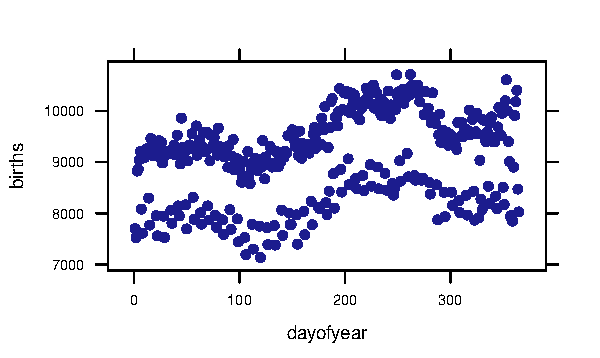
\includegraphics[width=\maxwidth]{figures/FrontMatter-unnamed-chunk-21-1} 

}



\end{knitrout}
From the \tab{Plots} tab, you can navigate to previous plots and also export plots 
in various formats after interactively resizing them.


% this fixes bad spacing -- but I don't know why the spacing was bad
%\bigskip
\subsection{The Packages Tab}

Much of the functionality of \R\ is located in packages, many of which can be obtained
from a central clearing house called CRAN (Comprehensive R Archive Network).  The \tab{Packages}
tab facilitates installing and loading packages.  It will also allow you to search for
packages that have been updated since you installed them.




\chapter{One Quantitative Variable}


\section{Numerical summaries}

\R\ includes a number of commands to numerically summarize variables.
These include the capability of calculating the mean, standard deviation,
variance, median, five number summary, interquartile range (IQR) as well as arbitrary quantiles.  We will
illustrate these using the CESD (Center for Epidemiologic Studies--Depression)
measure of depressive symptoms (which takes on values between 0 and 60, with higher
scores indicating more depressive symptoms).  

To improve the legibility of output,
we will also set the default number of digits to display to a more reasonable
level (see \function{?options} for more configuration possibilities).

\myindex{HELPrct dataset}%
\Rindex{options()}%
\Rindex{require()}%
\Rindex{mosaic package}%
\begin{knitrout}\small
\definecolor{shadecolor}{rgb}{1, 1, 1}\color{fgcolor}\begin{kframe}
\begin{alltt}
\hlstd{> }\hlkwd{require}\hlstd{(mosaic)}
\hlstd{> }\hlkwd{require}\hlstd{(mosaicData)}
\hlstd{> }\hlkwd{options}\hlstd{(}\hlkwc{digits}\hlstd{=}\hlnum{4}\hlstd{)}
\hlstd{> }\hlkwd{mean}\hlstd{(}\hlopt{~} \hlstd{cesd,} \hlkwc{data}\hlstd{=HELPrct)}
\end{alltt}
\begin{verbatim}
[1] 32.85
\end{verbatim}
\end{kframe}
\end{knitrout}

\myindex{Start Teaching with R@\emph{Start Teaching with R}}%
\myindex{Teaching with R@\emph{Teaching with R}}%
\myindex{Start Modeling with R@\emph{Start Modeling with R}}%
\myindex{Modeling with R@\emph{Modeling with R}}%
Note that the \function{mean()} function in the \pkg{mosaic} package supports a formula interface common to \pkg{lattice} graphics and linear models (e.g., \function{lm()}).  The \pkg{mosaic} package provides many other functions that use the same notation, which we will be using throughout this document.  
\DiggingDeeper[-3cm]{If you have not seen the formula notation before, the companion book, \emph{Start Teaching with R} provides a detailed presentation.  \emph{Start Modeling with R}, another companion book, details the relationship between the process of modeling and the formula notation. }

\Rindex{with()}%
\Rindex{mean()}%
The same output could be created using the following commands (though we will use the MOSAIC versions when available).
\begin{knitrout}\small
\definecolor{shadecolor}{rgb}{1, 1, 1}\color{fgcolor}\begin{kframe}
\begin{alltt}
\hlstd{> }\hlkwd{with}\hlstd{(HELPrct,} \hlkwd{mean}\hlstd{(cesd))}
\end{alltt}
\begin{verbatim}
[1] 32.85
\end{verbatim}
\begin{alltt}
\hlstd{> }\hlkwd{mean}\hlstd{(HELPrct}\hlopt{$}\hlstd{cesd)}
\end{alltt}
\begin{verbatim}
[1] 32.85
\end{verbatim}
\end{kframe}
\end{knitrout}
\Rindex{sd()}%
\Rindex{var()}%
Similar functionality exists for other summary statistics.
\begin{knitrout}\small
\definecolor{shadecolor}{rgb}{1, 1, 1}\color{fgcolor}\begin{kframe}
\begin{alltt}
\hlstd{> }\hlkwd{sd}\hlstd{(}\hlopt{~} \hlstd{cesd,} \hlkwc{data}\hlstd{=HELPrct)}
\end{alltt}
\begin{verbatim}
[1] 12.51
\end{verbatim}
\end{kframe}
\end{knitrout}
\begin{knitrout}\small
\definecolor{shadecolor}{rgb}{1, 1, 1}\color{fgcolor}\begin{kframe}
\begin{alltt}
\hlstd{> }\hlkwd{sd}\hlstd{(}\hlopt{~} \hlstd{cesd,} \hlkwc{data}\hlstd{=HELPrct)}\hlopt{^}\hlnum{2}
\end{alltt}
\begin{verbatim}
[1] 156.6
\end{verbatim}
\begin{alltt}
\hlstd{> }\hlkwd{var}\hlstd{(}\hlopt{~} \hlstd{cesd,} \hlkwc{data}\hlstd{=HELPrct)}
\end{alltt}
\begin{verbatim}
[1] 156.6
\end{verbatim}
\end{kframe}
\end{knitrout}

It is also straightforward to calculate quantiles of the distribution.

\myindex{quantiles}%
\Rindex{median()}%
\begin{knitrout}\small
\definecolor{shadecolor}{rgb}{1, 1, 1}\color{fgcolor}\begin{kframe}
\begin{alltt}
\hlstd{> }\hlkwd{median}\hlstd{(}\hlopt{~} \hlstd{cesd,} \hlkwc{data}\hlstd{=HELPrct)}
\end{alltt}
\begin{verbatim}
[1] 34
\end{verbatim}
\end{kframe}
\end{knitrout}

By default, the \function{quantile()} function displays the quartiles, but can be given a vector of quantiles to display.  
\Rindex{quantile()}%
\Caution{Not all commands have been upgraded to
support the formula interface. For these functions, variables within dataframes must be accessed using \function{with()} or the \$ operator.}
\begin{knitrout}\small
\definecolor{shadecolor}{rgb}{1, 1, 1}\color{fgcolor}\begin{kframe}
\begin{alltt}
\hlstd{> }\hlkwd{with}\hlstd{(HELPrct,} \hlkwd{quantile}\hlstd{(cesd))}
\end{alltt}
\begin{verbatim}
  0%  25%  50%  75% 100% 
   1   25   34   41   60 
\end{verbatim}
\begin{alltt}
\hlstd{> }\hlkwd{with}\hlstd{(HELPrct,} \hlkwd{quantile}\hlstd{(cesd,} \hlkwd{c}\hlstd{(}\hlnum{.025}\hlstd{,} \hlnum{.975}\hlstd{)))}
\end{alltt}
\begin{verbatim}
 2.5% 97.5% 
  6.3  55.0 
\end{verbatim}
\end{kframe}
\end{knitrout}

\hfill

\Rindex{favstats()}%
Finally, the \function{favstats()} function in the \pkg{mosaic} package provides a concise summary of  many useful statistics.
\begin{knitrout}\small
\definecolor{shadecolor}{rgb}{1, 1, 1}\color{fgcolor}\begin{kframe}
\begin{alltt}
\hlstd{> }\hlkwd{favstats}\hlstd{(}\hlopt{~} \hlstd{cesd,} \hlkwc{data}\hlstd{=HELPrct)}
\end{alltt}
\begin{verbatim}
 min Q1 median Q3 max  mean    sd   n missing
   1 25     34 41  60 32.85 12.51 453       0
\end{verbatim}
\end{kframe}
\end{knitrout}

\section{Graphical summaries}
The \function{histogram()} function is used to create a histogram. Here we use the formula interface (as discussed in the \emph{Start Modeling with R} book) to specify that we want a histogram of the CESD scores.

\Rindex{histogram()}%
\vspace{-4mm}
\begin{center}
\begin{knitrout}\small
\definecolor{shadecolor}{rgb}{1, 1, 1}\color{fgcolor}\begin{kframe}
\begin{alltt}
\hlstd{> }\hlkwd{gf_histogram}\hlstd{(}\hlopt{~} \hlstd{cesd,} \hlkwc{data} \hlstd{= HELPrct,} \hlkwc{binwidth} \hlstd{=} \hlnum{2.4}\hlstd{)} \hlopt
\hlstd{ }  \hlkwd{gf_labs}\hlstd{(}\hlkwc{title} \hlstd{=} \hlstr{""}\hlstd{)}
\end{alltt}
\end{kframe}

{\centering 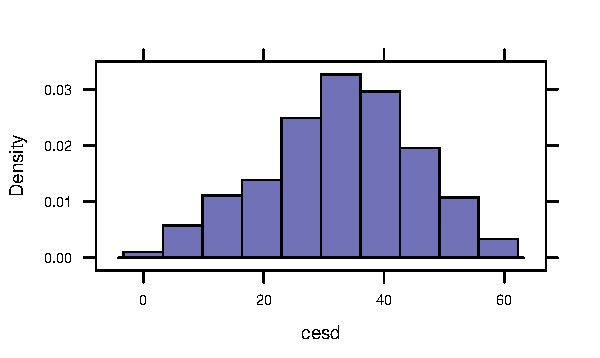
\includegraphics[width=\maxwidth]{figures/FrontMatter-cesd-hist-1} 

}



\end{knitrout}
\end{center}

We can use the \function{width} and \function{center} options to control the location of the bins.

\begin{center}
\begin{knitrout}\small
\definecolor{shadecolor}{rgb}{1, 1, 1}\color{fgcolor}\begin{kframe}
\begin{alltt}
\hlstd{> }\hlkwd{histogram}\hlstd{(}\hlopt{~} \hlstd{cesd,} \hlkwc{width}\hlstd{=}\hlnum{5}\hlstd{,} \hlkwc{center}\hlstd{=}\hlnum{2.5}\hlstd{,} \hlkwc{data}\hlstd{=HELPrct)}
\end{alltt}
\end{kframe}

{\centering 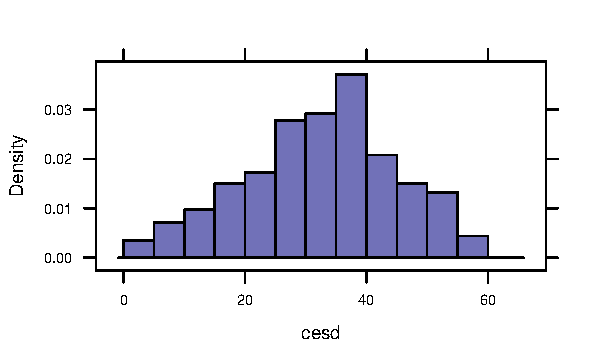
\includegraphics[width=\maxwidth]{figures/FrontMatter-cesd-hist2-1} 

}



\end{knitrout}
\end{center}


\Rindex{tally()}%
\Rindex{format option}%
In the \variable{HELPrct} dataset, approximately one quarter of the subjects are female.  
\begin{knitrout}\small
\definecolor{shadecolor}{rgb}{1, 1, 1}\color{fgcolor}\begin{kframe}
\begin{alltt}
\hlstd{> }\hlkwd{tally}\hlstd{(}\hlopt{~} \hlstd{sex,} \hlkwc{data}\hlstd{=HELPrct)}
\end{alltt}
\begin{verbatim}
sex
female   male 
   107    346 
\end{verbatim}
\begin{alltt}
\hlstd{> }\hlkwd{tally}\hlstd{(}\hlopt{~} \hlstd{sex,} \hlkwc{format}\hlstd{=}\hlstr{"percent"}\hlstd{,} \hlkwc{data}\hlstd{=HELPrct)}
\end{alltt}
\begin{verbatim}
sex
female   male 
 23.62  76.38 
\end{verbatim}
\end{kframe}
\end{knitrout}

It is straightforward to restrict our attention to just the female subjects.
If we are going to do many things with a subset of our data, it may be easiest
to make a new dataframe containing only the cases we are interested in.
The \function{filter()} function in the \pkg{dplyr} package can be used to generate a new dataframe containing
just the women or just the men  (see also section \ref{sec:subsets}).  Once this is created, the
the \function{stem()} function is used to create a stem and leaf plot.
\Caution{Note that the tests for equality use \emph{two} equal signs}
\Rindex{stem()}%
\Rindex{filter()}%
\Rindex{dplyr package}%
\begin{knitrout}\small
\definecolor{shadecolor}{rgb}{1, 1, 1}\color{fgcolor}\begin{kframe}
\begin{alltt}
\hlstd{> }\hlstd{female} \hlkwb{<-} \hlkwd{filter}\hlstd{(HELPrct, sex}\hlopt{==}\hlstr{'female'}\hlstd{)}
\hlstd{> }\hlstd{male} \hlkwb{<-} \hlkwd{filter}\hlstd{(HELPrct, sex}\hlopt{==}\hlstr{'male'}\hlstd{)}
\hlstd{> }\hlkwd{with}\hlstd{(female,} \hlkwd{stem}\hlstd{(cesd))}
\end{alltt}
\begin{verbatim}

  The decimal point is 1 digit(s) to the right of the |

  0 | 3
  0 | 567
  1 | 3
  1 | 555589999
  2 | 123344
  2 | 66889999
  3 | 0000233334444
  3 | 5556666777888899999
  4 | 00011112222334
  4 | 555666777889
  5 | 011122222333444
  5 | 67788
  6 | 0
\end{verbatim}
\end{kframe}
\end{knitrout}

\Rindex{dplyr package}%
\Rindex{tidyr package}%

Subsets can also be generated and used ``on the fly" (this time including
an overlaid normal density):
\Rindex{fit option}%
\begin{knitrout}\small
\definecolor{shadecolor}{rgb}{1, 1, 1}\color{fgcolor}\begin{kframe}
\begin{alltt}
\hlstd{> }\hlkwd{histogram}\hlstd{(}\hlopt{~} \hlstd{cesd,} \hlkwc{fit}\hlstd{=}\hlstr{"normal"}\hlstd{,}
\hlstd{ }  \hlkwc{data}\hlstd{=}\hlkwd{filter}\hlstd{(HELPrct, sex}\hlopt{==}\hlstr{'female'}\hlstd{))}
\end{alltt}
\end{kframe}

{\centering 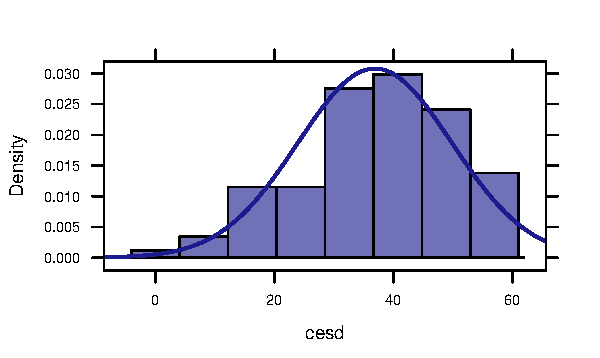
\includegraphics[width=\maxwidth]{figures/FrontMatter-women-cesd-hist-1} 

}



\end{knitrout}

Alternatively, we can make side-by-side plots to compare multiple subsets.
\begin{knitrout}\small
\definecolor{shadecolor}{rgb}{1, 1, 1}\color{fgcolor}\begin{kframe}
\begin{alltt}
\hlstd{> }\hlkwd{histogram}\hlstd{(}\hlopt{~} \hlstd{cesd} \hlopt{|} \hlstd{sex,} \hlkwc{data}\hlstd{=HELPrct)}
\end{alltt}
\end{kframe}

{\centering 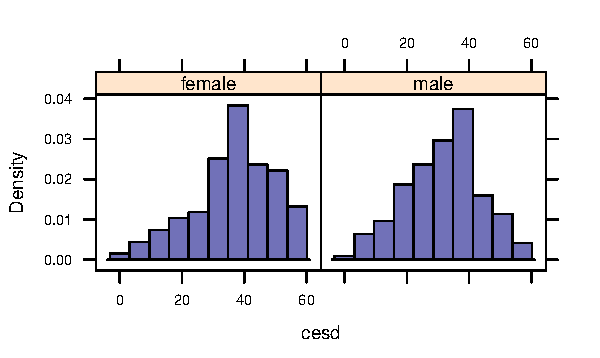
\includegraphics[width=\maxwidth]{figures/FrontMatter-cesd-male-female-1} 

}



\end{knitrout}

The layout can be rearranged.
\Rindex{layout option}%
\begin{center}
\begin{knitrout}\small
\definecolor{shadecolor}{rgb}{1, 1, 1}\color{fgcolor}\begin{kframe}
\begin{alltt}
\hlstd{> }\hlkwd{histogram}\hlstd{(}\hlopt{~} \hlstd{cesd} \hlopt{|} \hlstd{sex,} \hlkwc{layout}\hlstd{=}\hlkwd{c}\hlstd{(}\hlnum{1}\hlstd{,} \hlnum{2}\hlstd{),} \hlkwc{data}\hlstd{=HELPrct)}
\end{alltt}
\end{kframe}

{\centering 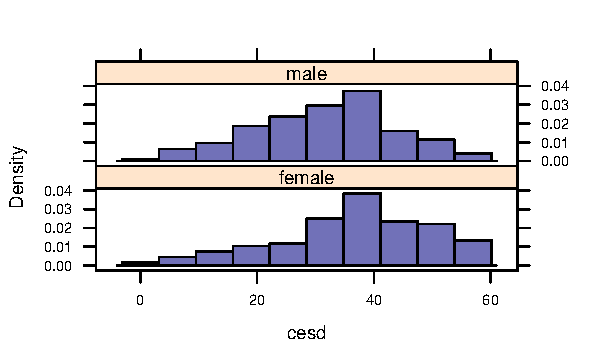
\includegraphics[width=\maxwidth]{figures/FrontMatter-cesd-dotlayout-1} 

}



\end{knitrout}
\end{center}
\begin{problem}
Using the \dataframe{HELPrct} dataset, 
create side-by-side histograms of the CESD scores by substance abuse
group, just for the male subjects, with an overlaid normal density.
\end{problem}%
\begin{solution}
\begin{knitrout}\small
\definecolor{shadecolor}{rgb}{1, 1, 1}\color{fgcolor}\begin{kframe}
\begin{alltt}
\hlstd{> }\hlkwd{histogram}\hlstd{(}\hlopt{~} \hlstd{cesd} \hlopt{|} \hlstd{substance,} \hlkwc{fit}\hlstd{=}\hlstr{"normal"}\hlstd{,}
\hlstd{ }  \hlkwc{data}\hlstd{=}\hlkwd{filter}\hlstd{(HELPrct, sex}\hlopt{==}\hlstr{'male'}\hlstd{))}
\end{alltt}
\end{kframe}

{\centering 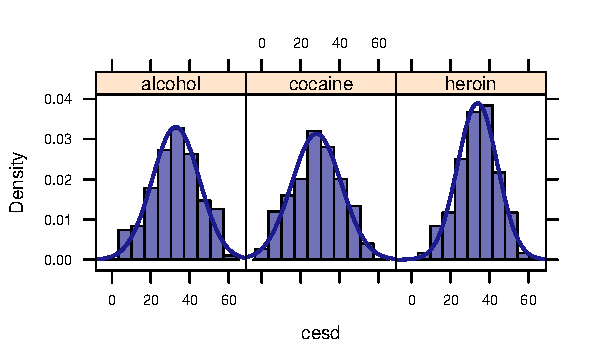
\includegraphics[width=\maxwidth]{figures/FrontMatter-subsmale-1} 

}



\end{knitrout}
\end{solution}%
We can control the number of bins in a number of ways.  These can be specified 
as the total number.
\Rindex{nint option}%
\begin{center}
\begin{knitrout}\small
\definecolor{shadecolor}{rgb}{1, 1, 1}\color{fgcolor}\begin{kframe}
\begin{alltt}
\hlstd{> }\hlkwd{histogram}\hlstd{(}\hlopt{~} \hlstd{cesd,} \hlkwc{nint}\hlstd{=}\hlnum{20}\hlstd{,} \hlkwc{data}\hlstd{=female)}
\end{alltt}
\end{kframe}

{\centering 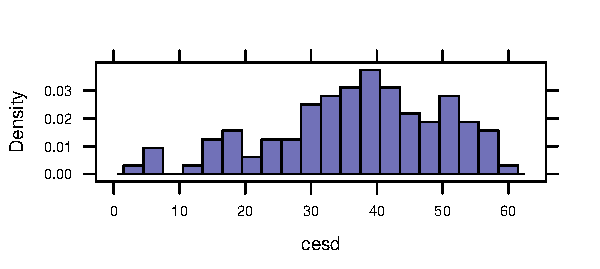
\includegraphics[width=\maxwidth]{figures/FrontMatter-cesd-dot-1} 

}



\end{knitrout}
\end{center}
The width of the bins can be specified.
\Rindex{width option}%
\begin{center}
\begin{knitrout}\small
\definecolor{shadecolor}{rgb}{1, 1, 1}\color{fgcolor}\begin{kframe}
\begin{alltt}
\hlstd{> }\hlkwd{histogram}\hlstd{(}\hlopt{~} \hlstd{cesd,} \hlkwc{width}\hlstd{=}\hlnum{2}\hlstd{,} \hlkwc{data}\hlstd{=female)}
\end{alltt}
\end{kframe}

{\centering 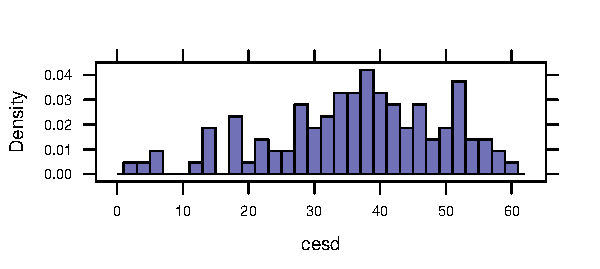
\includegraphics[width=\maxwidth]{figures/FrontMatter-cesd-dotwidth-1} 

}



\end{knitrout}
\end{center}

The \function{dotPlot()} function is used to create a dotplot
for a smaller subset of subjects (homeless females).  We also demonstrate
how to change the x-axis label.
\Rindex{dotPlot()}%
\begin{knitrout}\small
\definecolor{shadecolor}{rgb}{1, 1, 1}\color{fgcolor}\begin{kframe}
\begin{alltt}
\hlstd{> }\hlkwd{dotPlot}\hlstd{(}\hlopt{~} \hlstd{cesd,} \hlkwc{xlab}\hlstd{=}\hlstr{"CESD score"}\hlstd{,}
\hlstd{ }  \hlkwc{data}\hlstd{=}\hlkwd{filter}\hlstd{(HELPrct, (sex}\hlopt{==}\hlstr{"female"}\hlstd{)} \hlopt{&} \hlstd{(homeless}\hlopt{==}\hlstr{"homeless"}\hlstd{)))}
\end{alltt}
\end{kframe}

{\centering 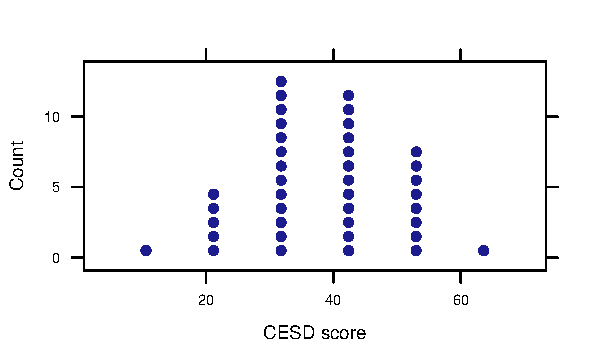
\includegraphics[width=\maxwidth]{figures/FrontMatter-cesd-dot4-1} 

}



\end{knitrout}


\section{Density curves}

\FoodForThought{Density plots are also sensitive to certain choices.  If your density plot is too jagged or too smooth, try changing the \option{adjust} argument: larger than 1 for smoother plots, less than 1 for more jagged plots.} One disadvantage of histograms is that they can be sensitive to the choice of the number of bins.  Another display to consider is a density curve.

Here we adorn a density plot with some additions to demonstrate how to build up a graphic for pedagogical purposes. We add some text, a superimposed normal density as well as a vertical line. A variety of line types and colors can be specified, as well as line widths.

\DiggingDeeper{The \function{plotFun()} function can also be used to annotate plots (see section \ref{sec:plotFun}).}
\begin{center}
\Rindex{densityplot()}%
\Rindex{ladd()}%
\Rindex{panel.mathdensity()}%
\Rindex{panel.abline()}%
\Rindex{col option}%
\Rindex{grid.text()}%
\Rindex{lty option}%
\Rindex{lwd option}%
\begin{knitrout}\small
\definecolor{shadecolor}{rgb}{1, 1, 1}\color{fgcolor}\begin{kframe}
\begin{alltt}
\hlstd{> }\hlkwd{densityplot}\hlstd{(}\hlopt{~} \hlstd{cesd,} \hlkwc{data}\hlstd{=female)}
\hlstd{> }\hlkwd{ladd}\hlstd{(}\hlkwd{grid.text}\hlstd{(}\hlkwc{x}\hlstd{=}\hlnum{0.2}\hlstd{,} \hlkwc{y}\hlstd{=}\hlnum{0.8}\hlstd{,} \hlstr{'only females'}\hlstd{))}
\hlstd{> }\hlkwd{ladd}\hlstd{(}\hlkwd{panel.mathdensity}\hlstd{(}\hlkwc{args}\hlstd{=}\hlkwd{list}\hlstd{(}\hlkwc{mean}\hlstd{=}\hlkwd{mean}\hlstd{(cesd),}
\hlstd{ }  \hlkwc{sd}\hlstd{=}\hlkwd{sd}\hlstd{(cesd)),} \hlkwc{col}\hlstd{=}\hlstr{"red"}\hlstd{),} \hlkwc{data}\hlstd{=female)}
\hlstd{> }\hlkwd{ladd}\hlstd{(}\hlkwd{panel.abline}\hlstd{(}\hlkwc{v}\hlstd{=}\hlnum{60}\hlstd{,} \hlkwc{lty}\hlstd{=}\hlnum{2}\hlstd{,} \hlkwc{lwd}\hlstd{=}\hlnum{2}\hlstd{,} \hlkwc{col}\hlstd{=}\hlstr{"grey"}\hlstd{))}
\end{alltt}
\end{kframe}

{\centering 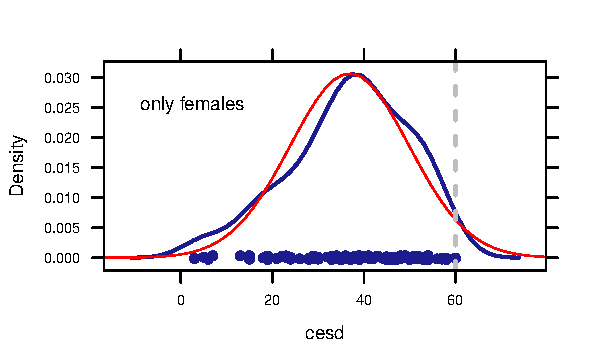
\includegraphics[width=\maxwidth]{figures/FrontMatter-dens1-1} 

}



\end{knitrout}
\end{center}

\section{Frequency polygons}
\myindex{polygons}%

A third option is a frequency polygon, where  the graph is created by joining the midpoints of the top of the bars of a histogram.
\Rindex{freqpolygon()}%
\begin{center}
\begin{knitrout}\small
\definecolor{shadecolor}{rgb}{1, 1, 1}\color{fgcolor}\begin{kframe}
\begin{alltt}
\hlstd{> }\hlkwd{freqpolygon}\hlstd{(}\hlopt{~} \hlstd{cesd,} \hlkwc{data}\hlstd{=female)}
\end{alltt}
\end{kframe}

{\centering 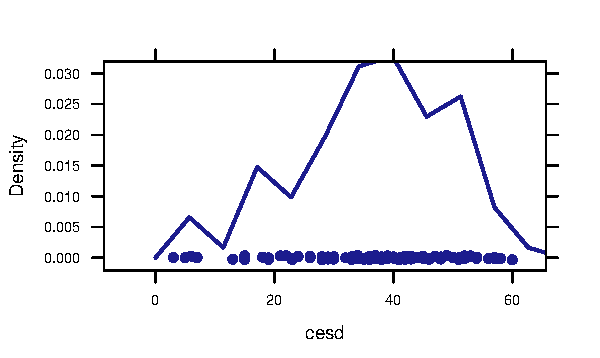
\includegraphics[width=2.5in]{figures/FrontMatter-poly-1} 

}



\end{knitrout}
\end{center}

\section{Normal distributions}

\FoodForThought{\code{x} is for eXtra.}%
The most famous density curve is a normal distribution.  The \function{xpnorm()} function displays the probability that a random variable is less than the first argument, for a normal distribution with mean given by the second argument and standard deviation by the third. More information about probability distributions can be found in section \ref{sec:probability}.

\begin{knitrout}\small
\definecolor{shadecolor}{rgb}{1, 1, 1}\color{fgcolor}\begin{kframe}
\begin{alltt}
\hlstd{> }\hlkwd{xpnorm}\hlstd{(}\hlnum{1.96}\hlstd{,} \hlkwc{mean}\hlstd{=}\hlnum{0}\hlstd{,} \hlkwc{sd}\hlstd{=}\hlnum{1}\hlstd{)}
\end{alltt}


{\ttfamily\noindent\itshape\color{messagecolor}{}}

{\ttfamily\noindent\itshape\color{messagecolor}{If X \textasciitilde{} N(0, 1), then }}

{\ttfamily\noindent\itshape\color{messagecolor}{	P(X <= 1.96) = P(Z <= 1.96) = 0.975}}

{\ttfamily\noindent\itshape\color{messagecolor}{	P(X >\ \ 1.96) = P(Z >\ \ 1.96) = 0.025}}

{\ttfamily\noindent\itshape\color{messagecolor}{}}\begin{verbatim}
[1] 0.975
\end{verbatim}
\end{kframe}

{\centering 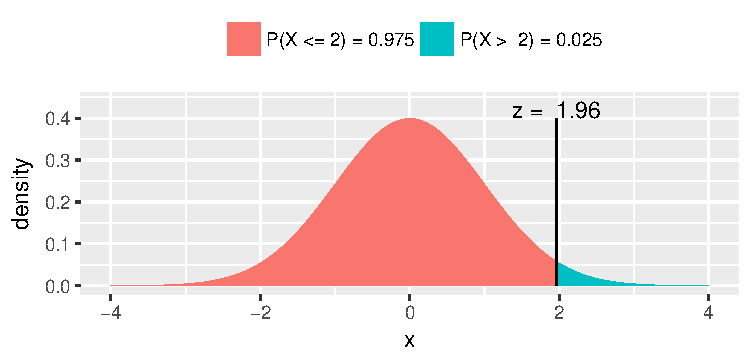
\includegraphics[width=\maxwidth]{figures/FrontMatter-norm1-1} 

}



\end{knitrout}


\section{Inference for a single sample}
\label{sec:bootstrapsing}

\Rindex{t.test()}%
\Rindex{confint()}%

We can calculate a 95\% confidence interval for the mean CESD 
score for females by using a t-test:
\begin{knitrout}\small
\definecolor{shadecolor}{rgb}{1, 1, 1}\color{fgcolor}\begin{kframe}
\begin{alltt}
\hlstd{> }\hlkwd{t.test}\hlstd{(}\hlopt{~} \hlstd{cesd,} \hlkwc{data}\hlstd{=female)}
\end{alltt}
\begin{verbatim}

	One Sample t-test

data:  cesd
t = 29, df = 110, p-value <2e-16
alternative hypothesis: true mean is not equal to 0
95 percent confidence interval:
 34.39 39.38
sample estimates:
mean of x 
    36.89 
\end{verbatim}
\begin{alltt}
\hlstd{> }\hlkwd{confint}\hlstd{(}\hlkwd{t.test}\hlstd{(}\hlopt{~} \hlstd{cesd,} \hlkwc{data}\hlstd{=female))}
\end{alltt}
\begin{verbatim}
  mean of x lower upper level
1     36.89 34.39 39.38  0.95
\end{verbatim}
\end{kframe}
\end{knitrout}

\DiggingDeeper{More details and examples can be found in the 
\pkg{mosaic} package Resampling Vignette.}
\myindex{bootstrapping}%
\myindex{resampling}%
But it's also straightforward to calculate this using a bootstrap.
The statistic that we want to resample is the mean.  
\begin{knitrout}\small
\definecolor{shadecolor}{rgb}{1, 1, 1}\color{fgcolor}\begin{kframe}
\begin{alltt}
\hlstd{> }\hlkwd{mean}\hlstd{(}\hlopt{~} \hlstd{cesd,} \hlkwc{data}\hlstd{=female)}
\end{alltt}
\begin{verbatim}
[1] 36.89
\end{verbatim}
\end{kframe}
\end{knitrout}

One resampling trial can be carried out:
\FoodForThought{Here we sample with replacement from the original dataframe,
creating a resampled dataframe with the same number of rows.}
\Rindex{resample()}%
\begin{knitrout}\small
\definecolor{shadecolor}{rgb}{1, 1, 1}\color{fgcolor}\begin{kframe}
\begin{alltt}
\hlstd{> }\hlkwd{mean}\hlstd{(}\hlopt{~} \hlstd{cesd,} \hlkwc{data}\hlstd{=}\hlkwd{resample}\hlstd{(female))}
\end{alltt}
\begin{verbatim}
[1] 37.7
\end{verbatim}
\end{kframe}
\end{knitrout}
\FoodForThought{Even though a single trial is of little use, it's smart having
students do the calculation to show that they are (usually!) getting a different
result than without resampling.}

Another will yield different results:
\begin{knitrout}\small
\definecolor{shadecolor}{rgb}{1, 1, 1}\color{fgcolor}\begin{kframe}
\begin{alltt}
\hlstd{> }\hlkwd{mean}\hlstd{(}\hlopt{~} \hlstd{cesd,} \hlkwc{data}\hlstd{=}\hlkwd{resample}\hlstd{(female))}
\end{alltt}
\begin{verbatim}
[1] 34.93
\end{verbatim}
\end{kframe}
\end{knitrout}

Now conduct 1000 resampling trials, saving the results in an object
called \texttt{trials}:
\Rindex{do()}%
\Rindex{qdata()}%
\begin{knitrout}\small
\definecolor{shadecolor}{rgb}{1, 1, 1}\color{fgcolor}\begin{kframe}
\begin{alltt}
\hlstd{> }\hlstd{trials} \hlkwb{<-} \hlkwd{do}\hlstd{(}\hlnum{1000}\hlstd{)} \hlopt{*} \hlkwd{mean}\hlstd{(}\hlopt{~} \hlstd{cesd,} \hlkwc{data}\hlstd{=}\hlkwd{resample}\hlstd{(female))}
\hlstd{> }\hlkwd{head}\hlstd{(trials,} \hlnum{3}\hlstd{)}
\end{alltt}
\begin{verbatim}
   mean
1 36.68
2 35.49
3 35.90
\end{verbatim}
\begin{alltt}
\hlstd{> }\hlkwd{qdata}\hlstd{(}\hlopt{~} \hlstd{mean,} \hlkwd{c}\hlstd{(}\hlnum{.025}\hlstd{,} \hlnum{.975}\hlstd{),} \hlkwc{data}\hlstd{=trials)}
\end{alltt}
\begin{verbatim}
      quantile     p
2.5%     34.27 0.025
97.5%    39.38 0.975
\end{verbatim}
\end{kframe}
\end{knitrout}

\chapter{One Categorical Variable}

\section{Numerical summaries}

\myindex{categorical variables}
\myindex{contingency tables}
\myindex{tables}

\DiggingDeeper{The \emph{Start Teaching with R} companion book introduces the formula notation used throughout this book. See also \emph{Start Teaching with R} for the connections to statistical modeling.}

The \function{tally()} function can be used to calculate
counts, percentages and proportions for a categorical variable.

\Rindex{tally()}%
\Rindex{margins option}%
\begin{knitrout}\small
\definecolor{shadecolor}{rgb}{1, 1, 1}\color{fgcolor}\begin{kframe}
\begin{alltt}
\hlstd{> }\hlkwd{tally}\hlstd{(}\hlopt{~} \hlstd{homeless,} \hlkwc{data}\hlstd{=HELPrct)}
\end{alltt}
\begin{verbatim}
homeless
homeless   housed 
     209      244 
\end{verbatim}
\begin{alltt}
\hlstd{> }\hlkwd{tally}\hlstd{(}\hlopt{~} \hlstd{homeless,} \hlkwc{margins}\hlstd{=}\hlnum{TRUE}\hlstd{,} \hlkwc{data}\hlstd{=HELPrct)}
\end{alltt}
\begin{verbatim}
homeless
homeless   housed    Total 
     209      244      453 
\end{verbatim}
\begin{alltt}
\hlstd{> }\hlkwd{tally}\hlstd{(}\hlopt{~} \hlstd{homeless,} \hlkwc{format}\hlstd{=}\hlstr{"percent"}\hlstd{,} \hlkwc{data}\hlstd{=HELPrct)}
\end{alltt}
\begin{verbatim}
homeless
homeless   housed 
   46.14    53.86 
\end{verbatim}
\begin{alltt}
\hlstd{> }\hlkwd{tally}\hlstd{(}\hlopt{~} \hlstd{homeless,} \hlkwc{format}\hlstd{=}\hlstr{"proportion"}\hlstd{,} \hlkwc{data}\hlstd{=HELPrct)}
\end{alltt}
\begin{verbatim}
homeless
homeless   housed 
  0.4614   0.5386 
\end{verbatim}
\end{kframe}
\end{knitrout}

\section{The binomial test}

\myindex{binomial test}%
\Rindex{binom.test()}%
An exact confidence interval for a proportion (as well as a test of the null 
hypothesis that the population proportion is equal to a particular value [by default 0.5]) can be calculated
using the \function{binom.test()} function.
The standard \function{binom.test()} requires us to tabulate.
\begin{knitrout}\small
\definecolor{shadecolor}{rgb}{1, 1, 1}\color{fgcolor}\begin{kframe}
\begin{alltt}
\hlstd{> }\hlkwd{binom.test}\hlstd{(}\hlnum{209}\hlstd{,} \hlnum{209} \hlopt{+} \hlnum{244}\hlstd{)}
\end{alltt}
\begin{verbatim}



data:  209 out of 209 + 244
number of successes = 210, number of trials = 450, p-value =
0.1
alternative hypothesis: true probability of success is not equal to 0.5
95 percent confidence interval:
 0.4147 0.5085
sample estimates:
probability of success 
                0.4614 
\end{verbatim}
\end{kframe}
\end{knitrout}
The \pkg{mosaic} package provides a formula interface that avoids the need to pre-tally
the data.
\begin{knitrout}\small
\definecolor{shadecolor}{rgb}{1, 1, 1}\color{fgcolor}\begin{kframe}
\begin{alltt}
\hlstd{> }\hlstd{result} \hlkwb{<-} \hlkwd{binom.test}\hlstd{(}\hlopt{~} \hlstd{(homeless}\hlopt{==}\hlstr{"homeless"}\hlstd{),} \hlkwc{data}\hlstd{=HELPrct)}
\hlstd{> }\hlstd{result}
\end{alltt}
\begin{verbatim}



data:  HELPrct$(homeless == "homeless")  [with success = TRUE]
number of successes = 210, number of trials = 450, p-value =
0.1
alternative hypothesis: true probability of success is not equal to 0.5
95 percent confidence interval:
 0.4147 0.5085
sample estimates:
probability of success 
                0.4614 
\end{verbatim}
\end{kframe}
\end{knitrout}

As is generally the case with commands of this sort, 
there are a number of useful quantities available from 
the object returned by the function.  
\begin{knitrout}\small
\definecolor{shadecolor}{rgb}{1, 1, 1}\color{fgcolor}\begin{kframe}
\begin{alltt}
\hlstd{> }\hlkwd{names}\hlstd{(result)}
\end{alltt}
\begin{verbatim}
[1] "statistic"   "parameter"   "p.value"     "conf.int"   
[5] "estimate"    "null.value"  "alternative" "data.name"  
\end{verbatim}
\end{kframe}
\end{knitrout}
These can be extracted using the {\tt \$} operator or an extractor function.
For example, the user can extract the confidence interval or p-value.
\Rindex{confint()}%
\Rindex{pval()}%
\Rindex{print()}%
\begin{knitrout}\small
\definecolor{shadecolor}{rgb}{1, 1, 1}\color{fgcolor}\begin{kframe}
\begin{alltt}
\hlstd{> }\hlstd{result}\hlopt{$}\hlstd{statistic}
\end{alltt}
\begin{verbatim}
number of successes 
                209 
\end{verbatim}
\begin{alltt}
\hlstd{> }\hlkwd{confint}\hlstd{(result)}
\end{alltt}
\begin{verbatim}
  probability of success  lower  upper level
1                 0.4614 0.4147 0.5085  0.95
\end{verbatim}
\begin{alltt}
\hlstd{> }\hlkwd{pval}\hlstd{(result)}
\end{alltt}
\begin{verbatim}
p.value 
 0.1101 
\end{verbatim}
\end{kframe}
\end{knitrout}
\DiggingDeeper{Most of the objects in \R\ have a \function{print()}
method.  So when we get \code{result}, what we are seeing displayed in the console is
\code{print(result)}.  There may be a good deal of additional information
lurking inside the object itself.  

In some situations, such as graphics, the object is returned \emph{invisibly}, so nothing prints.  That avoids your having to look at a long printout not intended for human consumption. You can still assign the returned object to a variable and process it later, even if nothing shows up on the screen.  This is sometimes helpful for \pkg{lattice} graphics functions.}%


\section{The proportion test}

A similar interval and test can be calculated using the function \function{prop.test()}.
\Rindex{prop.test()}%
\Rindex{correct option}%
Here is a count of the number of people at each of the two levels of \variable{homeless}

\begin{knitrout}\small
\definecolor{shadecolor}{rgb}{1, 1, 1}\color{fgcolor}\begin{kframe}
\begin{alltt}
\hlstd{> }\hlkwd{tally}\hlstd{(}\hlopt{~} \hlstd{homeless,} \hlkwc{data}\hlstd{=HELPrct)}
\end{alltt}
\begin{verbatim}
homeless
homeless   housed 
     209      244 
\end{verbatim}
\end{kframe}
\end{knitrout}

The \function{prop.test} function will carry out the calculations of the proportion test and report the result.

\hfill

\begin{knitrout}\small
\definecolor{shadecolor}{rgb}{1, 1, 1}\color{fgcolor}\begin{kframe}
\begin{alltt}
\hlstd{> }\hlkwd{prop.test}\hlstd{(}\hlopt{~} \hlstd{(homeless}\hlopt{==}\hlstr{"homeless"}\hlstd{),} \hlkwc{correct}\hlstd{=}\hlnum{FALSE}\hlstd{,} \hlkwc{data}\hlstd{=HELPrct)}
\end{alltt}
\begin{verbatim}

	1-sample proportions test without continuity correction

data:  HELPrct$(homeless == "homeless")  [with success = TRUE]
X-squared = 2.7, df = 1, p-value = 0.1
alternative hypothesis: true p is not equal to 0.5
95 percent confidence interval:
 0.4160 0.5074
sample estimates:
     p 
0.4614 
\end{verbatim}
\end{kframe}
\end{knitrout}
In this statement, prop.test is examining the \variable{homeless} variable in the same way that \function{tally} would. \Pointer{We write \code{homeless=="homeless"} to define unambiguously which proportion we are considering. We could also have written \code{homeless=="housed"}. }
\function{prop.test} can also work directly with numerical counts, the way \function{binom.test()} does.
\InstructorNote{\function{prop.test()} calculates a Chi-squared statistic.
Most introductory texts use a $z$-statistic.  They are mathematically equivalent in terms of inferential statements, but you may need to address the discrepancy with your students.}%
\begin{knitrout}\small
\definecolor{shadecolor}{rgb}{1, 1, 1}\color{fgcolor}\begin{kframe}
\begin{alltt}
\hlstd{> }\hlkwd{prop.test}\hlstd{(}\hlnum{209}\hlstd{,} \hlnum{209} \hlopt{+} \hlnum{244}\hlstd{,} \hlkwc{correct}\hlstd{=}\hlnum{FALSE}\hlstd{)}
\end{alltt}
\begin{verbatim}

	1-sample proportions test without continuity correction

data:  209 out of 209 + 244
X-squared = 2.7, df = 1, p-value = 0.1
alternative hypothesis: true p is not equal to 0.5
95 percent confidence interval:
 0.4160 0.5074
sample estimates:
     p 
0.4614 
\end{verbatim}
\end{kframe}
\end{knitrout}

\section{Goodness of fit tests}

A variety of goodness of fit tests can be calculated against a reference  distribution.  For the HELP data, we could test the null hypothesis that there is an equal proportion of subjects in each substance abuse group back in the original populations.


\begin{knitrout}\small
\definecolor{shadecolor}{rgb}{1, 1, 1}\color{fgcolor}\begin{kframe}
\begin{alltt}
\hlstd{> }\hlkwd{tally}\hlstd{(}\hlopt{~} \hlstd{substance,} \hlkwc{format}\hlstd{=}\hlstr{"percent"}\hlstd{,} \hlkwc{data}\hlstd{=HELPrct)}
\end{alltt}
\begin{verbatim}
substance
alcohol cocaine  heroin 
  39.07   33.55   27.37 
\end{verbatim}
\begin{alltt}
\hlstd{> }\hlstd{observed} \hlkwb{<-} \hlkwd{tally}\hlstd{(}\hlopt{~} \hlstd{substance,} \hlkwc{data}\hlstd{=HELPrct)}
\hlstd{> }\hlstd{observed}
\end{alltt}
\begin{verbatim}
substance
alcohol cocaine  heroin 
    177     152     124 
\end{verbatim}
\end{kframe}
\end{knitrout}

\Caution[-1cm]{In addition to the \option{format} option, there is an option \option{margins} to include marginal totals in the table. The default in \function{tally} is \option{margins=FALSE}. Try it out!}
\Rindex{chisq.test()}%
\begin{knitrout}\small
\definecolor{shadecolor}{rgb}{1, 1, 1}\color{fgcolor}\begin{kframe}
\begin{alltt}
\hlstd{> }\hlstd{p} \hlkwb{<-} \hlkwd{c}\hlstd{(}\hlnum{1}\hlopt{/}\hlnum{3}\hlstd{,} \hlnum{1}\hlopt{/}\hlnum{3}\hlstd{,} \hlnum{1}\hlopt{/}\hlnum{3}\hlstd{)}   \hlcom{# equivalent to rep(1/3, 3)}
\hlstd{> }\hlkwd{chisq.test}\hlstd{(observed,} \hlkwc{p}\hlstd{=p)}
\end{alltt}
\begin{verbatim}

	Chi-squared test for given probabilities

data:  observed
X-squared = 9.3, df = 2, p-value = 0.01
\end{verbatim}
\begin{alltt}
\hlstd{> }\hlstd{total} \hlkwb{<-} \hlkwd{sum}\hlstd{(observed); total}
\end{alltt}
\begin{verbatim}
[1] 453
\end{verbatim}
\begin{alltt}
\hlstd{> }\hlstd{expected} \hlkwb{<-} \hlstd{total}\hlopt{*}\hlstd{p; expected}
\end{alltt}
\begin{verbatim}
[1] 151 151 151
\end{verbatim}
\end{kframe}
\end{knitrout}

We can also calculate the $\chi^2$ statistic manually, as a function of observed and expected values.

\Rindex{sum()}%
\Rindex{pchisq()}%
\begin{knitrout}\small
\definecolor{shadecolor}{rgb}{1, 1, 1}\color{fgcolor}\begin{kframe}
\begin{alltt}
\hlstd{> }\hlstd{chisq} \hlkwb{<-} \hlkwd{sum}\hlstd{((observed} \hlopt{-} \hlstd{expected)}\hlopt{^}\hlnum{2}\hlopt{/}\hlstd{(expected)); chisq}
\end{alltt}
\begin{verbatim}
[1] 9.311
\end{verbatim}
\begin{alltt}
\hlstd{> }\hlnum{1} \hlopt{-} \hlkwd{pchisq}\hlstd{(chisq,} \hlkwc{df}\hlstd{=}\hlnum{2}\hlstd{)}
\end{alltt}
\begin{verbatim}
[1] 0.009508
\end{verbatim}
\end{kframe}
\end{knitrout}
\FoodForThought[-2cm]{The \function{pchisq} function calculates the probability that a $\chi^2$ random variable with \function{df} degrees is freedom is less than or equal to a given value.  Here we calculate the complement to find the area to the right of the observed Chi-square statistic.}%

It may be helpful to consult a graph of the statistic, where the shaded area represents the value to the right of the observed value.

\Rindex{plotDist()}%
\begin{knitrout}\small
\definecolor{shadecolor}{rgb}{1, 1, 1}\color{fgcolor}\begin{kframe}
\begin{alltt}
\hlstd{> }\hlkwd{plotDist}\hlstd{(}\hlstr{"chisq"}\hlstd{,} \hlkwc{df}\hlstd{=}\hlnum{2}\hlstd{,} \hlkwc{groups} \hlstd{= x} \hlopt{>} \hlnum{9.31}\hlstd{,} \hlkwc{type}\hlstd{=}\hlstr{"h"}\hlstd{)}
\end{alltt}
\end{kframe}

{\centering 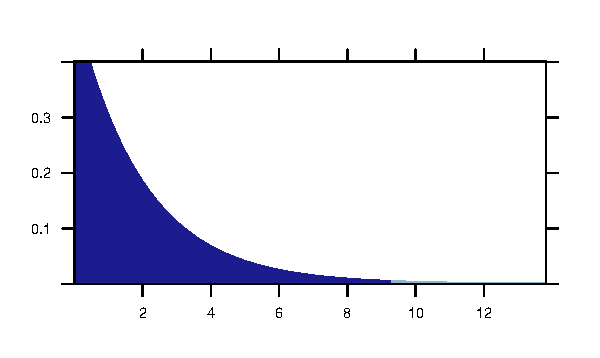
\includegraphics[width=\maxwidth]{figures/FrontMatter-chisqplotDist-1} 

}



\end{knitrout}


Alternatively, the \pkg{mosaic} package provides a version of \function{chisq.test()} with more verbose output.
\Rindex{xchisq.test()}%
\begin{knitrout}\small
\definecolor{shadecolor}{rgb}{1, 1, 1}\color{fgcolor}\begin{kframe}
\begin{alltt}
\hlstd{> }\hlkwd{xchisq.test}\hlstd{(observed,} \hlkwc{p}\hlstd{=p)}
\end{alltt}
\begin{verbatim}

	Chi-squared test for given probabilities

data:  x
X-squared = 9.3, df = 2, p-value = 0.01

  177      152      124   
(151.00) (151.00) (151.00)
[4.4768] [0.0066] [4.8278]
< 2.116> < 0.081> <-2.197>
     
key:
	observed
	(expected)
	[contribution to X-squared]
	<Pearson residual>
\end{verbatim}
\end{kframe}
\end{knitrout}
\FoodForThought[-1.5cm]{\code{x} in \function{xchisq.test} stands for eXtra.}

\FoodForThought{Objects in the workspace are listed in the {\sc Environment} tab in \RStudio.  If you want to clean up that listing, remove objects that are no longer needed with \function{rm}.}
\begin{knitrout}\small
\definecolor{shadecolor}{rgb}{1, 1, 1}\color{fgcolor}\begin{kframe}
\begin{alltt}
\hlstd{> }\hlcom{# clean up variables no longer needed}
\hlstd{> }\hlkwd{rm}\hlstd{(observed, p, total, chisq)}
\end{alltt}
\end{kframe}
\end{knitrout}

\chapter{Two Quantitative Variables}


\section{Scatterplots}
\myindex{scatterplots}%
\myindex{lowess}%
\myindex{smoothers}%
\myindex{linearity}%

We always encourage students to start any analysis by graphing their data.  
Here we augment a scatterplot
of the CESD (a measure of depressive symptoms, higher scores indicate more symptoms) and the MCS (mental component score from the SF-36, where higher scores indicate better functioning) for female subjects
with a lowess (locally weighted scatterplot smoother) line, using a circle
as the plotting character and slightly thicker line.

\InstructorNote{The lowess line can help to assess linearity of a relationship. This is added by specifying both points (using `p') and a lowess smoother.}
\Rindex{xyplot()}%
\Rindex{pch option}%
\Rindex{cex option}%
\Rindex{lwd option}%
\Rindex{type option}%
\begin{center}
\begin{knitrout}\small
\definecolor{shadecolor}{rgb}{1, 1, 1}\color{fgcolor}\begin{kframe}
\begin{alltt}
\hlstd{> }\hlstd{females} \hlkwb{<-} \hlkwd{filter}\hlstd{(HELPrct, female}\hlopt{==}\hlnum{1}\hlstd{)}
\hlstd{> }\hlkwd{xyplot}\hlstd{(cesd} \hlopt{~} \hlstd{mcs,} \hlkwc{type}\hlstd{=}\hlkwd{c}\hlstd{(}\hlstr{"p"}\hlstd{,}\hlstr{"smooth"}\hlstd{),} \hlkwc{pch}\hlstd{=}\hlnum{1}\hlstd{,}
\hlstd{ }  \hlkwc{cex}\hlstd{=}\hlnum{0.6}\hlstd{,} \hlkwc{lwd}\hlstd{=}\hlnum{3}\hlstd{,} \hlkwc{data}\hlstd{=females)}
\end{alltt}
\end{kframe}

{\centering 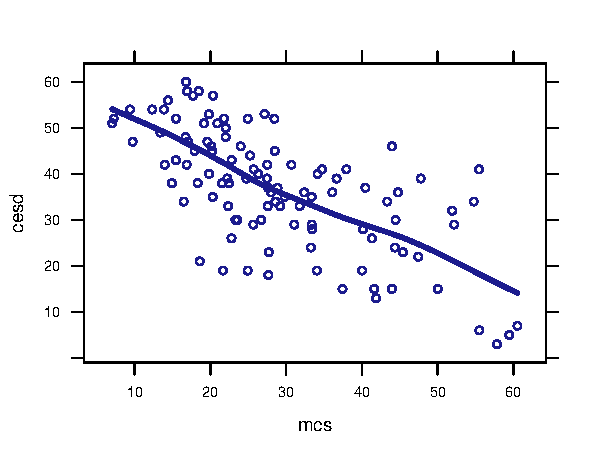
\includegraphics[width=\maxwidth]{figures/FrontMatter-HELPrct-xyplot-1} 

}



\end{knitrout}
\end{center}
\DiggingDeeper{The \emph{Start Modeling with R} companion book will be helpful if you are unfamiliar with the
modeling language.  The \emph{Start Teaching with R} also provides useful guidance in getting started.}

It's straightforward to plot something besides a character in a scatterplot.  
In this example, the \dataframe{USArrests} can be used to plot the association
between murder and assault rates, with the state name displayed.  This
requires a panel function to be written.
\Rindex{function()}%
\Rindex{panel.labels()}%
\Rindex{panel.text()}%
\Rindex{rownames()}%
\begin{knitrout}\small
\definecolor{shadecolor}{rgb}{1, 1, 1}\color{fgcolor}\begin{kframe}
\begin{alltt}
\hlstd{> }\hlstd{panel.labels} \hlkwb{<-} \hlkwa{function}\hlstd{(}\hlkwc{x}\hlstd{,} \hlkwc{y}\hlstd{,} \hlkwc{labels}\hlstd{=}\hlstr{'x'}\hlstd{,}\hlkwc{...}\hlstd{) \{}
\hlstd{ }  \hlkwd{panel.text}\hlstd{(x, y, labels,} \hlkwc{cex}\hlstd{=}\hlnum{0.4}\hlstd{, ...)}
\hlstd{ }\hlstd{\}}
\hlstd{> }\hlkwd{xyplot}\hlstd{(Murder} \hlopt{~} \hlstd{Assault,} \hlkwc{panel}\hlstd{=panel.labels,}
\hlstd{ }  \hlkwc{labels}\hlstd{=}\hlkwd{rownames}\hlstd{(USArrests),} \hlkwc{data}\hlstd{=USArrests)}
\end{alltt}
\end{kframe}

{\centering 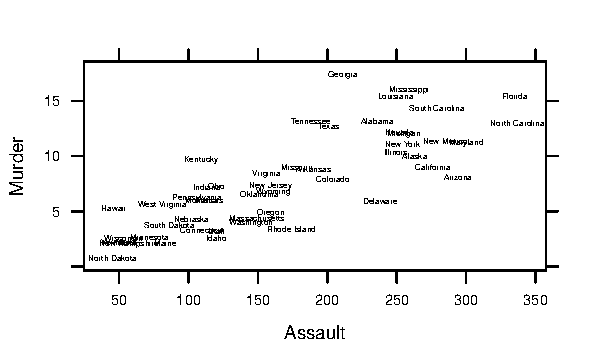
\includegraphics[width=\maxwidth]{figures/FrontMatter-unnamed-chunk-34-1} 

}



\end{knitrout}


\vspace*{-1cm}

\section{Correlation}


Correlations can be calculated for a pair of variables, or for a matrix of variables.
\myindex{correlation}%
\Rindex{cor()}%
\begin{knitrout}\small
\definecolor{shadecolor}{rgb}{1, 1, 1}\color{fgcolor}\begin{kframe}
\begin{alltt}
\hlstd{> }\hlkwd{cor}\hlstd{(cesd, mcs,} \hlkwc{data}\hlstd{=females)}
\end{alltt}


{\ttfamily\noindent\bfseries\color{errorcolor}{Error in typeof(x): object 'cesd' not found}}\begin{alltt}
\hlstd{> }\hlstd{smallHELP} \hlkwb{<-} \hlkwd{select}\hlstd{(females, cesd, mcs, pcs)}
\hlstd{> }\hlkwd{cor}\hlstd{(smallHELP)}
\end{alltt}
\begin{verbatim}
        cesd     mcs     pcs
cesd  1.0000 -0.6738 -0.3685
mcs  -0.6738  1.0000  0.2664
pcs  -0.3685  0.2664  1.0000
\end{verbatim}
\end{kframe}
\end{knitrout}
\myindex{Pearson correlation}%
\myindex{Spearman correlation}%

By default, Pearson correlations are provided. Other variants (e.g., Spearman) can be specified using the
\option{method} option.
\begin{knitrout}\small
\definecolor{shadecolor}{rgb}{1, 1, 1}\color{fgcolor}\begin{kframe}
\begin{alltt}
\hlstd{> }\hlkwd{cor}\hlstd{(cesd, mcs,} \hlkwc{method}\hlstd{=}\hlstr{"spearman"}\hlstd{,} \hlkwc{data}\hlstd{=females)}
\end{alltt}


{\ttfamily\noindent\bfseries\color{errorcolor}{Error in typeof(x): object 'cesd' not found}}\end{kframe}
\end{knitrout}

\section{Pairs plots}
\myindex{pairs plot}%
\myindex{scatterplot matrix}%

A pairs plot (scatterplot matrix) can be calculated for each pair of a set of variables.
\FoodForThought{The \pkg{GGally} package has support for more elaborate pairs plots.}
\Rindex{splom()}%
\begin{knitrout}\small
\definecolor{shadecolor}{rgb}{1, 1, 1}\color{fgcolor}\begin{kframe}
\begin{alltt}
\hlstd{> }\hlkwd{splom}\hlstd{(smallHELP,} \hlkwc{cex}\hlstd{=}\hlnum{0.3}\hlstd{)}
\end{alltt}
\end{kframe}

{\centering 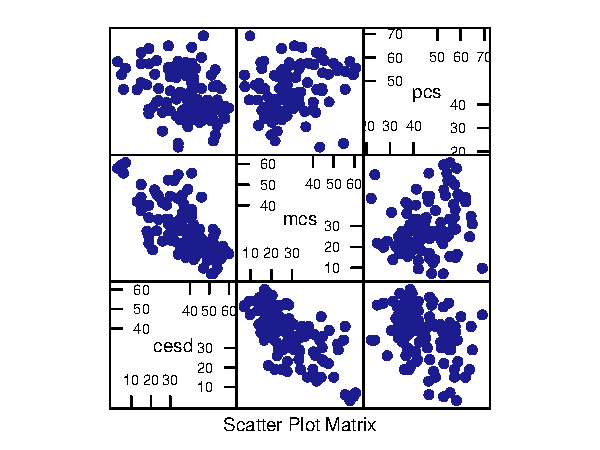
\includegraphics[width=\maxwidth]{figures/FrontMatter-unnamed-chunk-37-1} 

}



\end{knitrout}

\section{Simple linear regression}

\InstructorNote{We tend to introduce linear regression
early in our courses, as a purely descriptive technique.}
\myindex{linear regression}%
\myindex{regression}%

Linear regression models are described in detail in \emph{Start Modeling with R}.
These use the same formula interface introduced previously for numerical and graphical
summaries
to specify the outcome 
and predictors.  Here we consider fitting the model \model{\variable{cesd}}{\variable{mcs}}.


\Rindex{lm()}%
\Rindex{coef()}%
\begin{knitrout}\small
\definecolor{shadecolor}{rgb}{1, 1, 1}\color{fgcolor}\begin{kframe}
\begin{alltt}
\hlstd{> }\hlstd{cesdmodel} \hlkwb{<-} \hlkwd{lm}\hlstd{(cesd} \hlopt{~} \hlstd{mcs,} \hlkwc{data}\hlstd{=females)}
\hlstd{> }\hlkwd{coef}\hlstd{(cesdmodel)}
\end{alltt}
\begin{verbatim}
(Intercept)         mcs 
     57.349      -0.707 
\end{verbatim}
\end{kframe}
\end{knitrout}
\InstructorNote{It's important to pick good names for modeling
objects.  Here the output of \function{lm} is saved as \code{cesdmodel},
which denotes that it is a regression model of depressive symptom
scores.}

To simplify the output, we turn off the option to display significance stars.
\myindex{significance stars}%
\Rindex{msummary()}%
\Rindex{confint()}%
\Rindex{rsquared()}%
\Rindex{coef()}%
\begin{knitrout}\small
\definecolor{shadecolor}{rgb}{1, 1, 1}\color{fgcolor}\begin{kframe}
\begin{alltt}
\hlstd{> }\hlkwd{options}\hlstd{(}\hlkwc{show.signif.stars}\hlstd{=}\hlnum{FALSE}\hlstd{)}
\hlstd{> }\hlkwd{coef}\hlstd{(cesdmodel)}
\end{alltt}
\begin{verbatim}
(Intercept)         mcs 
     57.349      -0.707 
\end{verbatim}
\begin{alltt}
\hlstd{> }\hlkwd{msummary}\hlstd{(cesdmodel)}
\end{alltt}
\begin{verbatim}
            Estimate Std. Error t value Pr(>|t|)
(Intercept)  57.3485     2.3806   24.09  < 2e-16
mcs          -0.7070     0.0757   -9.34  1.8e-15

Residual standard error: 9.66 on 105 degrees of freedom
Multiple R-squared:  0.454,	Adjusted R-squared:  0.449 
F-statistic: 87.3 on 1 and 105 DF,  p-value: 1.81e-15
\end{verbatim}
\begin{alltt}
\hlstd{> }\hlkwd{coef}\hlstd{(}\hlkwd{summary}\hlstd{(cesdmodel))}
\end{alltt}
\begin{verbatim}
            Estimate Std. Error t value  Pr(>|t|)
(Intercept)   57.349    2.38062  24.090 1.425e-44
mcs           -0.707    0.07566  -9.344 1.813e-15
\end{verbatim}
\begin{alltt}
\hlstd{> }\hlkwd{confint}\hlstd{(cesdmodel)}
\end{alltt}
\begin{verbatim}
              2.5 % 97.5 %
(Intercept) 52.6282 62.069
mcs         -0.8571 -0.557
\end{verbatim}
\begin{alltt}
\hlstd{> }\hlkwd{rsquared}\hlstd{(cesdmodel)}
\end{alltt}
\begin{verbatim}
[1] 0.454
\end{verbatim}
\end{kframe}
\end{knitrout}


\Rindex{class()}%
\begin{knitrout}\small
\definecolor{shadecolor}{rgb}{1, 1, 1}\color{fgcolor}\begin{kframe}
\begin{alltt}
\hlstd{> }\hlkwd{class}\hlstd{(cesdmodel)}
\end{alltt}
\begin{verbatim}
[1] "lm"
\end{verbatim}
\end{kframe}
\end{knitrout}
The return value from \function{lm()} is a linear model object.
A number of functions can operate on these objects, as
seen previously with \function{coef()}.  
The function \function{residuals()} returns a
vector of the residuals.
\Rindex{residuals()}%
\FoodForThought{The function \function{residuals()} can be abbreviated 
\function{resid()}.  Another useful function is \function{fitted()}, which 
returns a vector of predicted values.}


\Rindex{density option}%
\begin{center}
\begin{knitrout}\small
\definecolor{shadecolor}{rgb}{1, 1, 1}\color{fgcolor}\begin{kframe}
\begin{alltt}
\hlstd{> }\hlkwd{histogram}\hlstd{(}\hlopt{~} \hlkwd{residuals}\hlstd{(cesdmodel),} \hlkwc{density}\hlstd{=}\hlnum{TRUE}\hlstd{)}
\end{alltt}
\end{kframe}

{\centering 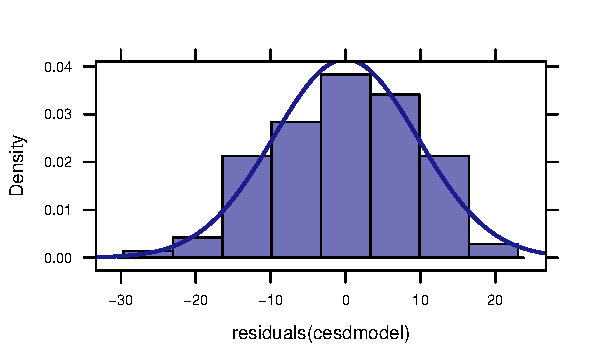
\includegraphics[width=\maxwidth]{figures/FrontMatter-lmhist-1} 

}



\end{knitrout}
\end{center}
\Rindex{qqmath()}%
\begin{center}
\begin{knitrout}\small
\definecolor{shadecolor}{rgb}{1, 1, 1}\color{fgcolor}\begin{kframe}
\begin{alltt}
\hlstd{> }\hlkwd{qqmath}\hlstd{(}\hlopt{~} \hlkwd{resid}\hlstd{(cesdmodel))}
\end{alltt}
\end{kframe}

{\centering 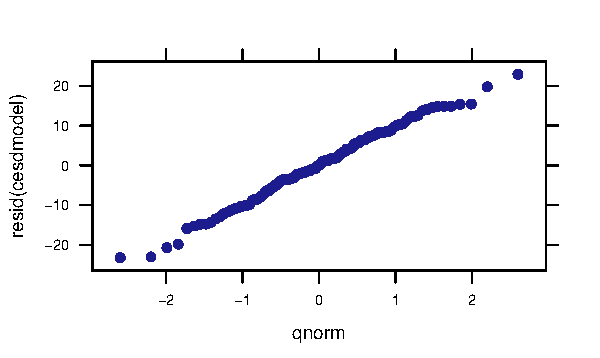
\includegraphics[width=\maxwidth]{figures/FrontMatter-HELPrct-resid-qq-1} 

}



\end{knitrout}
\end{center}
\Rindex{alpha option}%
\begin{center}
\begin{knitrout}\small
\definecolor{shadecolor}{rgb}{1, 1, 1}\color{fgcolor}\begin{kframe}
\begin{alltt}
\hlstd{> }\hlkwd{xyplot}\hlstd{(}\hlkwd{resid}\hlstd{(cesdmodel)} \hlopt{~} \hlkwd{fitted}\hlstd{(cesdmodel),} \hlkwc{type}\hlstd{=}\hlkwd{c}\hlstd{(}\hlstr{"p"}\hlstd{,} \hlstr{"smooth"}\hlstd{,} \hlstr{"r"}\hlstd{),}
\hlstd{ }       \hlkwc{alpha}\hlstd{=}\hlnum{0.5}\hlstd{,} \hlkwc{cex}\hlstd{=}\hlnum{0.3}\hlstd{,} \hlkwc{pch}\hlstd{=}\hlnum{20}\hlstd{)}
\end{alltt}
\end{kframe}

{\centering 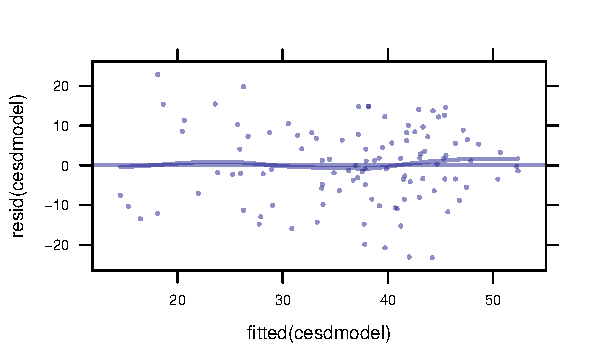
\includegraphics[width=\maxwidth]{figures/FrontMatter-HELPrct-resid-plot-1} 

}



\end{knitrout}
\end{center}

The \function{mplot()} function can facilitate creating a variety of useful plots, including the same residuals vs. fitted scatterplots, by specifying the \option{which=1} option.
\Rindex{mplot()}%
\Rindex{which option}%
\begin{knitrout}\small
\definecolor{shadecolor}{rgb}{1, 1, 1}\color{fgcolor}\begin{kframe}
\begin{alltt}
\hlstd{> }\hlkwd{mplot}\hlstd{(cesdmodel,} \hlkwc{which}\hlstd{=}\hlnum{1}\hlstd{)}
\end{alltt}
\begin{verbatim}
[[1]]
\end{verbatim}


{\ttfamily\noindent\itshape\color{messagecolor}{`geom\_smooth()` using method = 'loess'}}\end{kframe}


{\centering 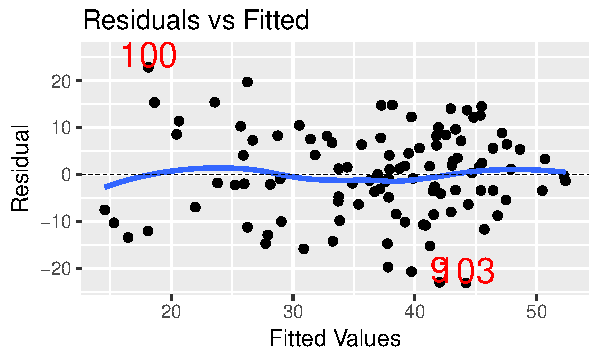
\includegraphics[width=\maxwidth]{figures/FrontMatter-mplotc1-1} 

}



\end{knitrout}

It can also generate a normal quantile-quantile plot (\option{which=2}),
\begin{knitrout}\small
\definecolor{shadecolor}{rgb}{1, 1, 1}\color{fgcolor}\begin{kframe}
\begin{alltt}
\hlstd{> }\hlkwd{mplot}\hlstd{(cesdmodel,} \hlkwc{which}\hlstd{=}\hlnum{2}\hlstd{)}
\end{alltt}
\end{kframe}

{\centering 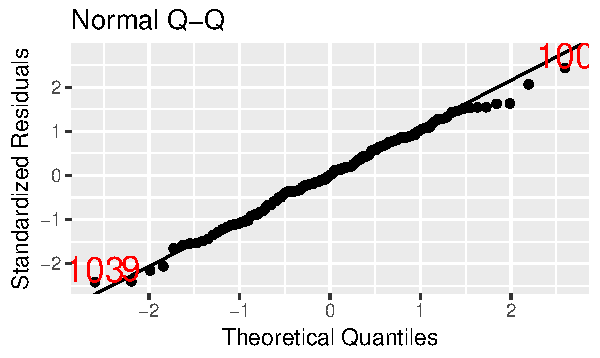
\includegraphics[width=\maxwidth]{figures/FrontMatter-mplotc2-1} 

}



\end{knitrout}

\myindex{scale versus location}%
scale vs.\,location,
\begin{knitrout}\small
\definecolor{shadecolor}{rgb}{1, 1, 1}\color{fgcolor}\begin{kframe}
\begin{alltt}
\hlstd{> }\hlkwd{mplot}\hlstd{(cesdmodel,} \hlkwc{which}\hlstd{=}\hlnum{3}\hlstd{)}
\end{alltt}


{\ttfamily\noindent\itshape\color{messagecolor}{`geom\_smooth()` using method = 'loess'}}\end{kframe}

{\centering 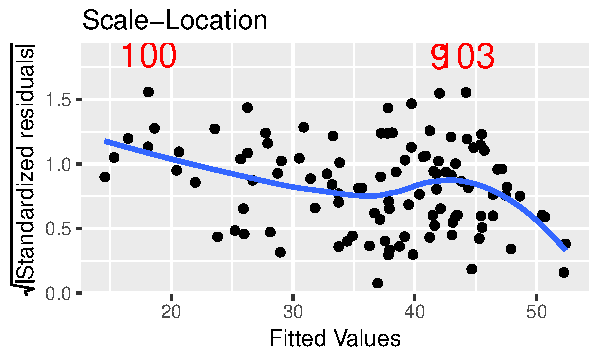
\includegraphics[width=\maxwidth]{figures/FrontMatter-mplotc3-1} 

}



\end{knitrout}

\myindex{Cook's distance}%
Cook's distance by observation number,
\begin{knitrout}\small
\definecolor{shadecolor}{rgb}{1, 1, 1}\color{fgcolor}\begin{kframe}
\begin{alltt}
\hlstd{> }\hlkwd{mplot}\hlstd{(cesdmodel,} \hlkwc{which}\hlstd{=}\hlnum{4}\hlstd{)}
\end{alltt}
\end{kframe}

{\centering 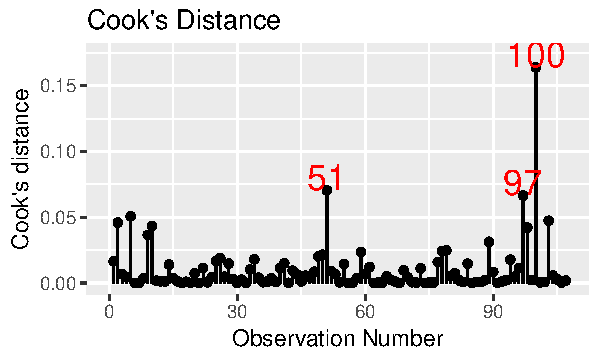
\includegraphics[width=\maxwidth]{figures/FrontMatter-mplotc4-1} 

}



\end{knitrout}

\myindex{leverage}%
residuals vs.\,leverage,
\begin{knitrout}\small
\definecolor{shadecolor}{rgb}{1, 1, 1}\color{fgcolor}\begin{kframe}
\begin{alltt}
\hlstd{> }\hlkwd{mplot}\hlstd{(cesdmodel,} \hlkwc{which}\hlstd{=}\hlnum{5}\hlstd{)}
\end{alltt}


{\ttfamily\noindent\itshape\color{messagecolor}{`geom\_smooth()` using method = 'loess'}}\end{kframe}

{\centering 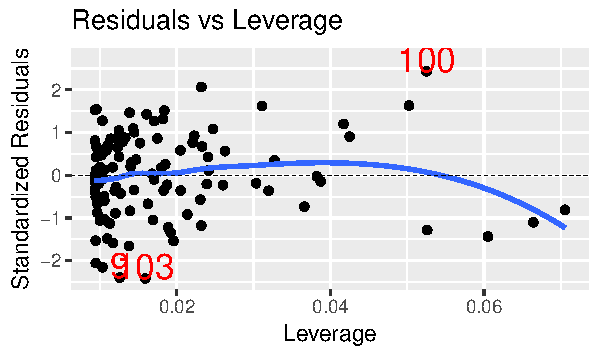
\includegraphics[width=\maxwidth]{figures/FrontMatter-mplotc5-1} 

}



\end{knitrout}

and Cook's distance vs. leverage.
\begin{knitrout}\small
\definecolor{shadecolor}{rgb}{1, 1, 1}\color{fgcolor}\begin{kframe}
\begin{alltt}
\hlstd{> }\hlkwd{mplot}\hlstd{(cesdmodel,} \hlkwc{which}\hlstd{=}\hlnum{6}\hlstd{)}
\end{alltt}


{\ttfamily\noindent\itshape\color{messagecolor}{`geom\_smooth()` using method = 'loess'}}\end{kframe}

{\centering 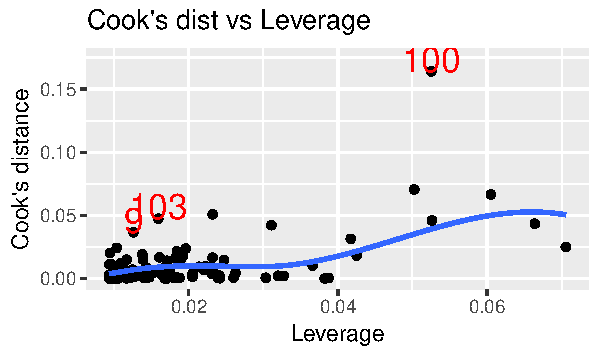
\includegraphics[width=\maxwidth]{figures/FrontMatter-mplotc6-1} 

}



\end{knitrout}

\myindex{prediction bands}%
\Rindex{panel.lmbands()}%
\Rindex{band.lwd option}%
Prediction bands can be added to a plot using the \function{panel.lmbands()} function.
\begin{center}
\begin{knitrout}\small
\definecolor{shadecolor}{rgb}{1, 1, 1}\color{fgcolor}\begin{kframe}
\begin{alltt}
\hlstd{> }\hlkwd{xyplot}\hlstd{(cesd} \hlopt{~} \hlstd{mcs,} \hlkwc{panel}\hlstd{=panel.lmbands,} \hlkwc{cex}\hlstd{=}\hlnum{0.2}\hlstd{,} \hlkwc{band.lwd}\hlstd{=}\hlnum{2}\hlstd{,} \hlkwc{data}\hlstd{=HELPrct)}
\end{alltt}
\end{kframe}

{\centering 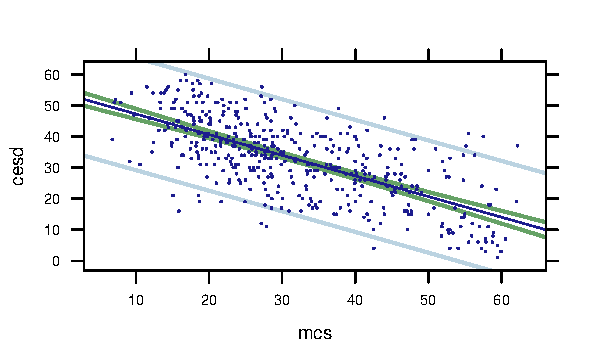
\includegraphics[width=\maxwidth]{figures/FrontMatter-HELPxyplot1-1} 

}



\end{knitrout}
\end{center}

\begin{problem}
Using the \dataframe{HELPrct} dataset, fit a simple linear regression model 
predicting the number of drinks per day as a function of the mental
component score.  
This model can be specified using the formula:
\model{\variable{i1}}{\variable{mcs}}.  
Assess the distribution of the residuals for this model.
\end{problem}


\chapter{Two Categorical Variables}


\section{Cross classification tables}
\label{sec:cross}

\myindex{cross classification tables}%
\myindex{contingency tables}%
\myindex{tables}%

Cross classification (two-way or $R$ by $C$) tables can be constructed for
two (or more) categorical variables.  Here we consider the contingency table
for homeless status (homeless one or more nights in the past 6 months or housed) 
and sex.

\begin{knitrout}\small
\definecolor{shadecolor}{rgb}{1, 1, 1}\color{fgcolor}\begin{kframe}
\begin{alltt}
\hlstd{> }\hlkwd{tally}\hlstd{(}\hlopt{~} \hlstd{homeless} \hlopt{+} \hlstd{sex,} \hlkwc{margins}\hlstd{=}\hlnum{FALSE}\hlstd{,} \hlkwc{data}\hlstd{=HELPrct)}
\end{alltt}
\begin{verbatim}
          sex
homeless   female male
  homeless     40  169
  housed       67  177
\end{verbatim}
\end{kframe}
\end{knitrout}

We can also calculate column percentages:
\Rindex{tally()}%
\begin{knitrout}\small
\definecolor{shadecolor}{rgb}{1, 1, 1}\color{fgcolor}\begin{kframe}
\begin{alltt}
\hlstd{> }\hlkwd{tally}\hlstd{(}\hlopt{~} \hlstd{sex} \hlopt{|} \hlstd{homeless,} \hlkwc{margins}\hlstd{=}\hlnum{TRUE}\hlstd{,} \hlkwc{format}\hlstd{=}\hlstr{"percent"}\hlstd{,}
\hlstd{ }  \hlkwc{data}\hlstd{=HELPrct)}
\end{alltt}
\begin{verbatim}
        homeless
sex      homeless housed
  female    19.14  27.46
  male      80.86  72.54
  Total    100.00 100.00
\end{verbatim}
\end{kframe}
\end{knitrout}

We can calculate the odds ratio directly from the table:
\begin{knitrout}\small
\definecolor{shadecolor}{rgb}{1, 1, 1}\color{fgcolor}\begin{kframe}
\begin{alltt}
\hlstd{> }\hlstd{OR} \hlkwb{<-} \hlstd{(}\hlnum{40}\hlopt{/}\hlnum{169}\hlstd{)}\hlopt{/}\hlstd{(}\hlnum{67}\hlopt{/}\hlnum{177}\hlstd{); OR}
\end{alltt}
\begin{verbatim}
[1] 0.6253
\end{verbatim}
\end{kframe}
\end{knitrout}

The
\pkg{mosaic} package has a function which will calculate odds ratios:
\Rindex{oddsRatio()}%
\begin{knitrout}\small
\definecolor{shadecolor}{rgb}{1, 1, 1}\color{fgcolor}\begin{kframe}
\begin{alltt}
\hlstd{> }\hlkwd{oddsRatio}\hlstd{(}\hlkwd{tally}\hlstd{(}\hlopt{~} \hlstd{(homeless}\hlopt{==}\hlstr{"housed"}\hlstd{)} \hlopt{+} \hlstd{sex,} \hlkwc{margins}\hlstd{=}\hlnum{FALSE}\hlstd{,}
\hlstd{ }  \hlkwc{data}\hlstd{=HELPrct))}
\end{alltt}
\begin{verbatim}
[1] 0.6253
\end{verbatim}
\end{kframe}
\end{knitrout}

The \function{CrossTable()} function in the \pkg{gmodels} package also displays
a cross classification table.

\Rindex{CrossTable()}%
\begin{knitrout}\small
\definecolor{shadecolor}{rgb}{1, 1, 1}\color{fgcolor}\begin{kframe}
\begin{alltt}
\hlstd{> }\hlkwd{require}\hlstd{(gmodels)}
\hlstd{> }\hlkwd{with}\hlstd{(HELPrct,} \hlkwd{CrossTable}\hlstd{(homeless, sex,}
\hlstd{ }  \hlkwc{prop.r}\hlstd{=}\hlnum{FALSE}\hlstd{,} \hlkwc{prop.chisq}\hlstd{=}\hlnum{FALSE}\hlstd{,} \hlkwc{prop.t}\hlstd{=}\hlnum{FALSE}\hlstd{))}
\end{alltt}
\begin{verbatim}

 
   Cell Contents
|-------------------------|
|                       N |
|           N / Col Total |
|-------------------------|

 
Total Observations in Table:  453 

 
             | sex 
    homeless |    female |      male | Row Total | 
-------------|-----------|-----------|-----------|
    homeless |        40 |       169 |       209 | 
             |     0.374 |     0.488 |           | 
-------------|-----------|-----------|-----------|
      housed |        67 |       177 |       244 | 
             |     0.626 |     0.512 |           | 
-------------|-----------|-----------|-----------|
Column Total |       107 |       346 |       453 | 
             |     0.236 |     0.764 |           | 
-------------|-----------|-----------|-----------|

 
\end{verbatim}
\end{kframe}
\end{knitrout}

Graphical summaries of cross classification tables may be helpful in visualizing
associations.  Mosaic plots are one example, where the total area (all observations) is proportional to one.
\Caution{The jury is still out
regarding the utility of mosaic plots (also known as eikosograms), 
relative to the low data to ink ratio.\cite{Tufte:2001:Visual}%
We have found them to be helpful to reinforce understanding of a two way contingency table.}%
Here we see that males tend to be over-represented
amongst the homeless subjects (as represented by the horizontal line which is higher for
the homeless rather than the housed).  
\FoodForThought{The \function{mosaic()} function 
in the \pkg{vcd} package also makes mosaic plots.}
\Rindex{mosaicplot()}%
\begin{center}
\begin{knitrout}\small
\definecolor{shadecolor}{rgb}{1, 1, 1}\color{fgcolor}\begin{kframe}
\begin{alltt}
\hlstd{> }\hlstd{mytab} \hlkwb{<-} \hlkwd{tally}\hlstd{(}\hlopt{~} \hlstd{homeless} \hlopt{+} \hlstd{sex,} \hlkwc{margins}\hlstd{=}\hlnum{FALSE}\hlstd{,}
\hlstd{ }  \hlkwc{data}\hlstd{=HELPrct)}
\hlstd{> }\hlkwd{mosaicplot}\hlstd{(mytab)}
\end{alltt}
\end{kframe}

{\centering 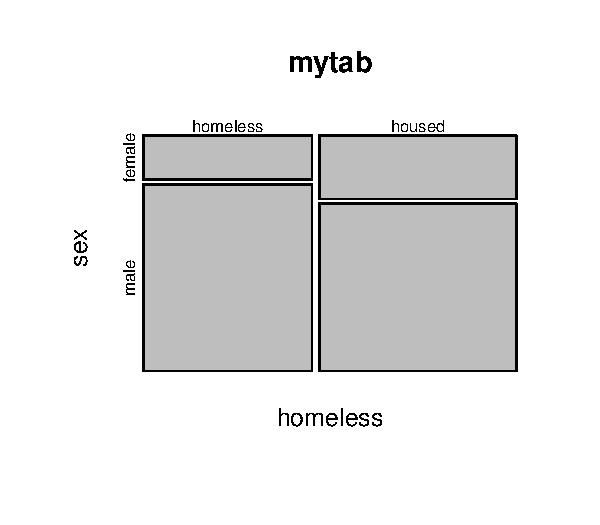
\includegraphics[width=\maxwidth]{figures/FrontMatter-mosaicplot-1} 

}



\end{knitrout}
\end{center}

\section{Creating tables from summary statistics}

Tables can be created from summary statistics using the \function{do} function.

\begin{knitrout}\small
\definecolor{shadecolor}{rgb}{1, 1, 1}\color{fgcolor}\begin{kframe}
\begin{alltt}
\hlstd{> }\hlstd{HELPtable} \hlkwb{<-} \hlkwd{rbind}\hlstd{(}
\hlstd{ }  \hlkwd{do}\hlstd{(}\hlnum{40}\hlstd{)}  \hlopt{*} \hlkwd{data.frame}\hlstd{(}\hlkwc{sex}\hlstd{=}\hlstr{"female"}\hlstd{,} \hlkwc{homeless}\hlstd{=}\hlstr{"homeless"}\hlstd{),}
\hlstd{ }  \hlkwd{do}\hlstd{(}\hlnum{169}\hlstd{)} \hlopt{*} \hlkwd{data.frame}\hlstd{(}\hlkwc{sex}\hlstd{=}\hlstr{"male"}\hlstd{,}   \hlkwc{homeless}\hlstd{=}\hlstr{"homeless"}\hlstd{),}
\hlstd{ }  \hlkwd{do}\hlstd{(}\hlnum{67}\hlstd{)}  \hlopt{*} \hlkwd{data.frame}\hlstd{(}\hlkwc{sex}\hlstd{=}\hlstr{"female"}\hlstd{,} \hlkwc{homeless}\hlstd{=}\hlstr{"housed"}\hlstd{),}
\hlstd{ }  \hlkwd{do}\hlstd{(}\hlnum{177}\hlstd{)} \hlopt{*} \hlkwd{data.frame}\hlstd{(}\hlkwc{sex}\hlstd{=}\hlstr{"male"}\hlstd{,}   \hlkwc{homeless}\hlstd{=}\hlstr{"housed"}\hlstd{)}
\hlstd{ }\hlstd{)}
\hlstd{> }\hlkwd{tally}\hlstd{(}\hlopt{~} \hlstd{homeless} \hlopt{+} \hlstd{sex,} \hlkwc{data}\hlstd{=HELPtable)}
\end{alltt}
\begin{verbatim}
          sex
homeless   female male
  homeless     40  169
  housed       67  177
\end{verbatim}
\end{kframe}
\end{knitrout}

\section{Chi-squared tests}

\Rindex{chisq.test()}%
\begin{knitrout}\small
\definecolor{shadecolor}{rgb}{1, 1, 1}\color{fgcolor}\begin{kframe}
\begin{alltt}
\hlstd{> }\hlkwd{chisq.test}\hlstd{(}\hlkwd{tally}\hlstd{(}\hlopt{~} \hlstd{homeless} \hlopt{+} \hlstd{sex,} \hlkwc{margins}\hlstd{=}\hlnum{FALSE}\hlstd{,}
\hlstd{ }  \hlkwc{data}\hlstd{=HELPrct),} \hlkwc{correct}\hlstd{=}\hlnum{FALSE}\hlstd{)}
\end{alltt}
\begin{verbatim}

	Pearson's Chi-squared test

data:  tally(~homeless + sex, margins = FALSE, data = HELPrct)
X-squared = 4.3, df = 1, p-value = 0.04
\end{verbatim}
\end{kframe}
\end{knitrout}

There is a statistically significant association found: it is unlikely that we would observe
an association this strong if homeless status and sex were independent in the 
population.

When a student finds a significant association, 
it's important for them to be able to interpret this in the context of the problem. 
The \function{xchisq.test()} function provides additional details (observed, expected, contribution to statistic, and residual) to help with this process.
\FoodForThought{\code{x} is for eXtra.}

\Rindex{xchisq.test()}%
\begin{knitrout}\small
\definecolor{shadecolor}{rgb}{1, 1, 1}\color{fgcolor}\begin{kframe}
\begin{alltt}
\hlstd{> }\hlkwd{xchisq.test}\hlstd{(}\hlkwd{tally}\hlstd{(}\hlopt{~}\hlstd{homeless} \hlopt{+} \hlstd{sex,} \hlkwc{margins}\hlstd{=}\hlnum{FALSE}\hlstd{,}
\hlstd{ }  \hlkwc{data}\hlstd{=HELPrct),} \hlkwc{correct}\hlstd{=}\hlnum{FALSE}\hlstd{)}
\end{alltt}
\begin{verbatim}

	Pearson's Chi-squared test

data:  x
X-squared = 4.3, df = 1, p-value = 0.04

   40      169   
( 49.37) (159.63)
 [1.78]   [0.55] 
<-1.33>  < 0.74> 
   
   67      177   
( 57.63) (186.37)
 [1.52]   [0.47] 
< 1.23>  <-0.69> 
   
key:
	observed
	(expected)
	[contribution to X-squared]
	<Pearson residual>
\end{verbatim}
\end{kframe}
\end{knitrout}

We observe that there are fewer homeless women, and more homeless men that would be expected.

\section{Fisher's exact test}
\myindex{Fisher's exact test}%

An exact test can also be calculated.  This is computationally straightforward for 2 by 2
tables.  Options to help constrain the size of the problem for larger tables exist
(see \verb!?fisher.test()!).

\DiggingDeeper{Note the different estimate of the odds ratio from that seen in section \ref{sec:cross}.
The \function{fisher.test()} function uses a different estimator (and different interval based 
on the profile likelihood).}
\Rindex{fisher.test()}%
\begin{knitrout}\small
\definecolor{shadecolor}{rgb}{1, 1, 1}\color{fgcolor}\begin{kframe}
\begin{alltt}
\hlstd{> }\hlkwd{fisher.test}\hlstd{(}\hlkwd{tally}\hlstd{(}\hlopt{~}\hlstd{homeless} \hlopt{+} \hlstd{sex,} \hlkwc{margins}\hlstd{=}\hlnum{FALSE}\hlstd{,}
\hlstd{ }  \hlkwc{data}\hlstd{=HELPrct))}
\end{alltt}
\begin{verbatim}

	Fisher's Exact Test for Count Data

data:  tally(~homeless + sex, margins = FALSE, data = HELPrct)
p-value = 0.05
alternative hypothesis: true odds ratio is not equal to 1
95 percent confidence interval:
 0.3895 0.9968
sample estimates:
odds ratio 
    0.6259 
\end{verbatim}
\end{kframe}
\end{knitrout}

\chapter{Quantitative Response, Categorical Predictor}


\section{A dichotomous predictor: numerical and graphical summaries}
Here we will compare the distributions of CESD scores by sex.
The \function{mean()} function can be used to calculate the mean CESD score
separately for males and females.
\Rindex{mean()}%
\begin{knitrout}\small
\definecolor{shadecolor}{rgb}{1, 1, 1}\color{fgcolor}\begin{kframe}
\begin{alltt}
\hlstd{> }\hlkwd{mean}\hlstd{(cesd} \hlopt{~} \hlstd{sex,} \hlkwc{data}\hlstd{=HELPrct)}
\end{alltt}
\begin{verbatim}
female   male 
 36.89  31.60 
\end{verbatim}
\end{kframe}
\end{knitrout}
\Rindex{favstats()}%
The \function{favstats()} function can provide more statistics by group.

\begin{knitrout}\small
\definecolor{shadecolor}{rgb}{1, 1, 1}\color{fgcolor}\begin{kframe}
\begin{alltt}
\hlstd{> }\hlkwd{favstats}\hlstd{(cesd} \hlopt{~} \hlstd{sex,} \hlkwc{data}\hlstd{=HELPrct)}
\end{alltt}
\begin{verbatim}
     sex min Q1 median   Q3 max  mean    sd   n missing
1 female   3 29   38.0 46.5  60 36.89 13.02 107       0
2   male   1 24   32.5 40.0  58 31.60 12.10 346       0
\end{verbatim}
\end{kframe}
\end{knitrout}


Boxplots are a particularly helpful graphical display to compare distributions.
The \function{bwplot()} function can be used to display the boxplots for the
CESD scores separately by sex.  We see from both the numerical and graphical
summaries that women tend to have slightly higher CESD scores than men.

\FoodForThought[-3cm]{Although we usually put explanatory variables along the horizontal axis,
page layout sometimes makes the other orientation preferable for these plots.}
%\vspace{-8mm}
\Rindex{bwplot()}%
\begin{center}
\begin{knitrout}\small
\definecolor{shadecolor}{rgb}{1, 1, 1}\color{fgcolor}\begin{kframe}
\begin{alltt}
\hlstd{> }\hlkwd{bwplot}\hlstd{(sex} \hlopt{~} \hlstd{cesd,} \hlkwc{data}\hlstd{=HELPrct)}
\end{alltt}
\end{kframe}

{\centering 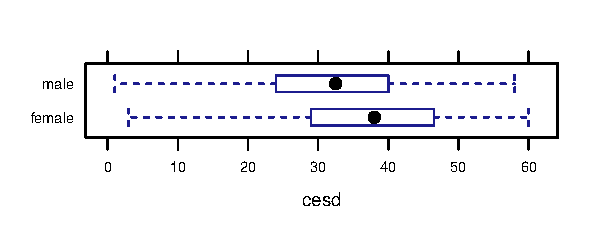
\includegraphics[width=\maxwidth]{figures/FrontMatter-cesd-box-1} 

}



\end{knitrout}
\end{center}

When sample sizes are small, there is no reason to summarize with a boxplot
since  \function{xyplot()} can handle categorical predictors.
Even with 10--20 observations in a group, a scatter plot is often quite readable.
Setting the alpha level helps detect multiple observations with the same value.
\FoodForThought{One of us once saw a biologist proudly present
side-by-side boxplots.  Thinking a major victory had been won, he naively
asked how many observations were in each group.  ``Four,'' replied the 
biologist.}
\Rindex{xyplot()}%
\Rindex{alpha option}%
\Rindex{cex option}%
\begin{center}
\begin{knitrout}\small
\definecolor{shadecolor}{rgb}{1, 1, 1}\color{fgcolor}\begin{kframe}
\begin{alltt}
\hlstd{> }\hlkwd{xyplot}\hlstd{(sex} \hlopt{~} \hlstd{length,} \hlkwc{alpha}\hlstd{=}\hlnum{.6}\hlstd{,} \hlkwc{cex}\hlstd{=}\hlnum{1.4}\hlstd{,} \hlkwc{data}\hlstd{=KidsFeet)}
\end{alltt}
\end{kframe}

{\centering 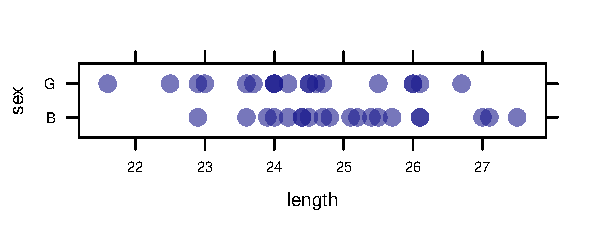
\includegraphics[width=\maxwidth]{figures/FrontMatter-KidsFeet-xy-1} 

}



\end{knitrout}
\end{center}

\section{A dichotomous predictor: two-sample t}

The Student's two sample t-test can be run without (default) or with an equal variance assumption.
\Rindex{t.test()}%
\Rindex{var.equal option}%
\begin{knitrout}\small
\definecolor{shadecolor}{rgb}{1, 1, 1}\color{fgcolor}\begin{kframe}
\begin{alltt}
\hlstd{> }\hlkwd{t.test}\hlstd{(cesd} \hlopt{~} \hlstd{sex,} \hlkwc{var.equal}\hlstd{=}\hlnum{FALSE}\hlstd{,} \hlkwc{data}\hlstd{=HELPrct)}
\end{alltt}
\begin{verbatim}

	Welch Two Sample t-test

data:  cesd by sex
t = 3.7, df = 170, p-value = 3e-04
alternative hypothesis: true difference in means is not equal to 0
95 percent confidence interval:
 2.493 8.087
sample estimates:
mean in group female   mean in group male 
               36.89                31.60 
\end{verbatim}
\end{kframe}
\end{knitrout}
We see that there is a statistically significant difference between the two groups.

We can repeat using the equal variance assumption.
\begin{knitrout}\small
\definecolor{shadecolor}{rgb}{1, 1, 1}\color{fgcolor}\begin{kframe}
\begin{alltt}
\hlstd{> }\hlkwd{t.test}\hlstd{(cesd} \hlopt{~} \hlstd{sex,} \hlkwc{var.equal}\hlstd{=}\hlnum{TRUE}\hlstd{,} \hlkwc{data}\hlstd{=HELPrct)}
\end{alltt}
\begin{verbatim}

	Two Sample t-test

data:  cesd by sex
t = 3.9, df = 450, p-value = 1e-04
alternative hypothesis: true difference in means is not equal to 0
95 percent confidence interval:
 2.610 7.969
sample estimates:
mean in group female   mean in group male 
               36.89                31.60 
\end{verbatim}
\end{kframe}
\end{knitrout}

The groups can also be compared using the \function{lm()} function (also with an equal variance assumption).  The mosaic command \function{msummary()} provides a slightly terser version of the typical output from \function{summary()}.
\Rindex{msummary()}%
\Rindex{summary()}%
\begin{knitrout}\small
\definecolor{shadecolor}{rgb}{1, 1, 1}\color{fgcolor}\begin{kframe}
\begin{alltt}
\hlstd{> }\hlkwd{msummary}\hlstd{(}\hlkwd{lm}\hlstd{(cesd} \hlopt{~} \hlstd{sex,} \hlkwc{data}\hlstd{=HELPrct))}
\end{alltt}
\begin{verbatim}
            Estimate Std. Error t value Pr(>|t|)
(Intercept)    36.89       1.19   30.96  < 2e-16
sexmale        -5.29       1.36   -3.88  0.00012

Residual standard error: 12.3 on 451 degrees of freedom
Multiple R-squared:  0.0323,	Adjusted R-squared:  0.0302 
F-statistic: 15.1 on 1 and 451 DF,  p-value: 0.00012
\end{verbatim}
\end{kframe}
\end{knitrout}

\FoodForThought[1cm]{The \function{lm} function is part of a much more flexible modeling framework while \function{t.test} is essentially a dead end. \function{lm} uses of the equal variance assumption. See the companion book, {\em Start Modeling in R} for more details.}%


\section{Non-parametric 2 group tests}

The same conclusion is reached using a non-parametric (Wilcoxon rank sum) test.

\Rindex{wilcox.test()}%
\begin{knitrout}\small
\definecolor{shadecolor}{rgb}{1, 1, 1}\color{fgcolor}\begin{kframe}
\begin{alltt}
\hlstd{> }\hlkwd{wilcox.test}\hlstd{(cesd} \hlopt{~} \hlstd{sex,} \hlkwc{data}\hlstd{=HELPrct)}
\end{alltt}
\begin{verbatim}

	Wilcoxon rank sum test with continuity correction

data:  cesd by sex
W = 23000, p-value = 1e-04
alternative hypothesis: true location shift is not equal to 0
\end{verbatim}
\end{kframe}
\end{knitrout}


\section{Permutation test}
\myindex{resampling}%
\myindex{permutation test}%


Here we extend the methods introduced in section \ref{sec:bootstrapsing} to 
undertake a two-sided test comparing the ages at baseline by gender.  First we calculate the observed difference in means:
\Rindex{diffmean()}%
\Rindex{shuffle()}%
\begin{knitrout}\small
\definecolor{shadecolor}{rgb}{1, 1, 1}\color{fgcolor}\begin{kframe}
\begin{alltt}
\hlstd{> }\hlkwd{mean}\hlstd{(age} \hlopt{~} \hlstd{sex,} \hlkwc{data}\hlstd{=HELPrct)}
\end{alltt}
\begin{verbatim}
female   male 
 36.25  35.47 
\end{verbatim}
\begin{alltt}
\hlstd{> }\hlstd{test.stat} \hlkwb{<-} \hlkwd{diffmean}\hlstd{(age} \hlopt{~} \hlstd{sex,} \hlkwc{data}\hlstd{=HELPrct)}
\hlstd{> }\hlstd{test.stat}
\end{alltt}
\begin{verbatim}
diffmean 
 -0.7841 
\end{verbatim}
\end{kframe}
\end{knitrout}
We can calculate the same statistic after shuffling the group labels:
\begin{knitrout}\small
\definecolor{shadecolor}{rgb}{1, 1, 1}\color{fgcolor}\begin{kframe}
\begin{alltt}
\hlstd{> }\hlkwd{do}\hlstd{(}\hlnum{1}\hlstd{)} \hlopt{*} \hlkwd{diffmean}\hlstd{(age} \hlopt{~} \hlkwd{shuffle}\hlstd{(sex),} \hlkwc{data}\hlstd{=HELPrct)}
\end{alltt}
\begin{verbatim}
  diffmean
1   0.2682
\end{verbatim}
\begin{alltt}
\hlstd{> }\hlkwd{do}\hlstd{(}\hlnum{1}\hlstd{)} \hlopt{*} \hlkwd{diffmean}\hlstd{(age} \hlopt{~} \hlkwd{shuffle}\hlstd{(sex),} \hlkwc{data}\hlstd{=HELPrct)}
\end{alltt}
\begin{verbatim}
  diffmean
1  0.03568
\end{verbatim}
\begin{alltt}
\hlstd{> }\hlkwd{do}\hlstd{(}\hlnum{3}\hlstd{)} \hlopt{*} \hlkwd{diffmean}\hlstd{(age} \hlopt{~} \hlkwd{shuffle}\hlstd{(sex),} \hlkwc{data}\hlstd{=HELPrct)}
\end{alltt}
\begin{verbatim}
  diffmean
1  -0.5149
2  -0.6128
3   0.3049
\end{verbatim}
\end{kframe}
\end{knitrout}

\DiggingDeeper{More details and examples can be found in the
\pkg{mosaic} package Resampling Vignette.}
\Rindex{xlim option}%
\Rindex{groups option}%
\begin{knitrout}\small
\definecolor{shadecolor}{rgb}{1, 1, 1}\color{fgcolor}\begin{kframe}
\begin{alltt}
\hlstd{> }\hlstd{rtest.stats} \hlkwb{<-} \hlkwd{do}\hlstd{(}\hlnum{500}\hlstd{)} \hlopt{*} \hlkwd{diffmean}\hlstd{(age} \hlopt{~} \hlkwd{shuffle}\hlstd{(sex),}
\hlstd{ }  \hlkwc{data}\hlstd{=HELPrct)}
\hlstd{> }\hlkwd{head}\hlstd{(rtest.stats,} \hlnum{3}\hlstd{)}
\end{alltt}
\begin{verbatim}
  diffmean
1 -0.14786
2  0.31711
3  0.04792
\end{verbatim}
\begin{alltt}
\hlstd{> }\hlkwd{favstats}\hlstd{(}\hlopt{~} \hlstd{diffmean,} \hlkwc{data}\hlstd{=rtest.stats)}
\end{alltt}
\begin{verbatim}
    min      Q1  median     Q3   max    mean     sd   n missing
 -2.204 -0.5272 0.06015 0.6475 2.299 0.05017 0.8714 500       0
\end{verbatim}
\begin{alltt}
\hlstd{> }\hlkwd{histogram}\hlstd{(}\hlopt{~} \hlstd{diffmean,} \hlkwc{n}\hlstd{=}\hlnum{40}\hlstd{,} \hlkwc{xlim}\hlstd{=}\hlkwd{c}\hlstd{(}\hlopt{-}\hlnum{6}\hlstd{,} \hlnum{6}\hlstd{),}
\hlstd{ }  \hlkwc{groups}\hlstd{=diffmean} \hlopt{>=} \hlstd{test.stat,} \hlkwc{pch}\hlstd{=}\hlnum{16}\hlstd{,} \hlkwc{cex}\hlstd{=}\hlnum{.8}\hlstd{,}
\hlstd{ }  \hlkwc{data}\hlstd{=rtest.stats)}
\hlstd{> }\hlkwd{ladd}\hlstd{(}\hlkwd{panel.abline}\hlstd{(}\hlkwc{v}\hlstd{=test.stat,} \hlkwc{lwd}\hlstd{=}\hlnum{3}\hlstd{,} \hlkwc{col}\hlstd{=}\hlstr{"red"}\hlstd{))}
\end{alltt}
\end{kframe}

{\centering 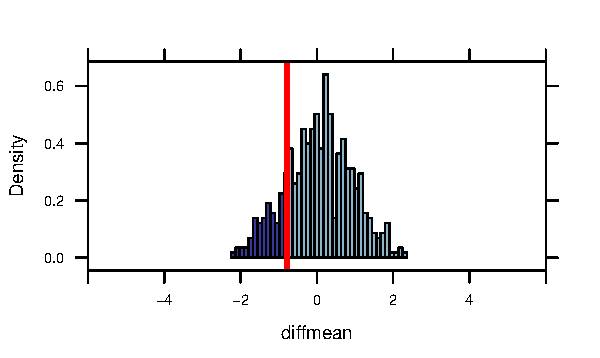
\includegraphics[width=\maxwidth]{figures/FrontMatter-permute-HELPrct-1} 

}



\end{knitrout}

Here we don't see much evidence to contradict the null hypothesis that men and 
women 
have the same mean age in the population.

\section{One-way ANOVA}
\myindex{one-way ANOVA}%
\myindex{analysis of variance}%

Earlier comparisons were between two groups. We can also consider testing differences between
three or more groups using one-way ANOVA.  Here we compare
CESD scores by primary substance of abuse (heroin, cocaine, or alcohol) with a line rather a dot to indicate the median.

\Rindex{bwplot()}%
\begin{center}
\begin{knitrout}\small
\definecolor{shadecolor}{rgb}{1, 1, 1}\color{fgcolor}\begin{kframe}
\begin{alltt}
\hlstd{> }\hlkwd{bwplot}\hlstd{(cesd} \hlopt{~} \hlstd{substance,} \hlkwc{pch}\hlstd{=}\hlstr{"|"}\hlstd{,} \hlkwc{data}\hlstd{=HELPrct)}
\end{alltt}
\end{kframe}

{\centering 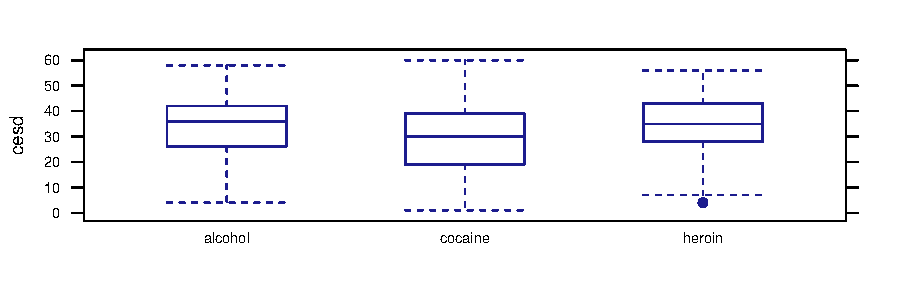
\includegraphics[width=\maxwidth]{figures/FrontMatter-cesd-oneway-1} 

}



\end{knitrout}
\end{center}



\begin{knitrout}\small
\definecolor{shadecolor}{rgb}{1, 1, 1}\color{fgcolor}\begin{kframe}
\begin{alltt}
\hlstd{> }\hlkwd{mean}\hlstd{(cesd} \hlopt{~} \hlstd{substance,} \hlkwc{data}\hlstd{=HELPrct)}
\end{alltt}
\begin{verbatim}
alcohol cocaine  heroin 
  34.37   29.42   34.87 
\end{verbatim}
\end{kframe}
\end{knitrout}
\Rindex{aov()}%
\begin{knitrout}\small
\definecolor{shadecolor}{rgb}{1, 1, 1}\color{fgcolor}\begin{kframe}
\begin{alltt}
\hlstd{> }\hlstd{anovamod} \hlkwb{<-} \hlkwd{aov}\hlstd{(cesd} \hlopt{~} \hlstd{substance,} \hlkwc{data}\hlstd{=HELPrct)}
\hlstd{> }\hlkwd{summary}\hlstd{(anovamod)}
\end{alltt}
\begin{verbatim}
             Df Sum Sq Mean Sq F value  Pr(>F)
substance     2   2704    1352    8.94 0.00016
Residuals   450  68084     151                
\end{verbatim}
\end{kframe}
\end{knitrout}
While still high (scores of 16 or more are generally considered to be 
``severe'' symptoms), the cocaine-involved group tend to have lower 
scores than those whose primary substances are alcohol or heroin.
\begin{knitrout}\small
\definecolor{shadecolor}{rgb}{1, 1, 1}\color{fgcolor}\begin{kframe}
\begin{alltt}
\hlstd{> }\hlstd{modintercept} \hlkwb{<-} \hlkwd{lm}\hlstd{(cesd} \hlopt{~} \hlnum{1}\hlstd{,} \hlkwc{data}\hlstd{=HELPrct)}
\hlstd{> }\hlstd{modsubstance} \hlkwb{<-} \hlkwd{lm}\hlstd{(cesd} \hlopt{~} \hlstd{substance,} \hlkwc{data}\hlstd{=HELPrct)}
\end{alltt}
\end{kframe}
\end{knitrout}

The \function{anova()} command can summarize models.
\Rindex{anova()}%
\begin{knitrout}\small
\definecolor{shadecolor}{rgb}{1, 1, 1}\color{fgcolor}\begin{kframe}
\begin{alltt}
\hlstd{> }\hlkwd{anova}\hlstd{(modsubstance)}
\end{alltt}
\begin{verbatim}
Analysis of Variance Table

Response: cesd
           Df Sum Sq Mean Sq F value  Pr(>F)
substance   2   2704    1352    8.94 0.00016
Residuals 450  68084     151                
\end{verbatim}
\end{kframe}
\end{knitrout}

In this setting the results are identical (since there is only one predictor, with 2 df).

The \function{anova()} function can also be used to formally 
compare two (nested) models.
\myindex{model comparison}%
\begin{knitrout}\small
\definecolor{shadecolor}{rgb}{1, 1, 1}\color{fgcolor}\begin{kframe}
\begin{alltt}
\hlstd{> }\hlkwd{anova}\hlstd{(modintercept, modsubstance)}
\end{alltt}
\begin{verbatim}
Analysis of Variance Table

Model 1: cesd ~ 1
Model 2: cesd ~ substance
  Res.Df   RSS Df Sum of Sq    F  Pr(>F)
1    452 70788                          
2    450 68084  2      2704 8.94 0.00016
\end{verbatim}
\end{kframe}
\end{knitrout}


\section{Tukey's Honest Significant Differences}
\myindex{Tukey's HSD}%
\myindex{honest significant differences}%
\myindex{multiple comparisons}%

There are a variety of multiple comparison procedures that can be
used after fitting an ANOVA model.  One of these is Tukey's Honest
Significant Differences (HSD).  Other options are available within the 
\pkg{multcomp} package.

\begin{knitrout}\small
\definecolor{shadecolor}{rgb}{1, 1, 1}\color{fgcolor}\begin{kframe}
\begin{alltt}
\hlstd{> }\hlkwd{favstats}\hlstd{(cesd} \hlopt{~} \hlstd{substance,} \hlkwc{data}\hlstd{=HELPrct)}
\end{alltt}
\begin{verbatim}
  substance min Q1 median Q3 max  mean    sd   n missing
1   alcohol   4 26     36 42  58 34.37 12.05 177       0
2   cocaine   1 19     30 39  60 29.42 13.40 152       0
3    heroin   4 28     35 43  56 34.87 11.20 124       0
\end{verbatim}
\end{kframe}
\end{knitrout}
\Rindex{TukeyHSD()}%
\Rindex{factor()}%
\Rindex{levels option}%
\Rindex{labels option}%
\Rindex{mutate()}%
\Rindex{lm()}%
\begin{knitrout}\small
\definecolor{shadecolor}{rgb}{1, 1, 1}\color{fgcolor}\begin{kframe}
\begin{alltt}
\hlstd{> }\hlstd{HELPrct} \hlkwb{<-} \hlkwd{mutate}\hlstd{(HELPrct,} \hlkwc{subgrp} \hlstd{=} \hlkwd{factor}\hlstd{(substance,}
\hlstd{ }  \hlkwc{levels}\hlstd{=}\hlkwd{c}\hlstd{(}\hlstr{"alcohol"}\hlstd{,} \hlstr{"cocaine"}\hlstd{,} \hlstr{"heroin"}\hlstd{),}
\hlstd{ }  \hlkwc{labels}\hlstd{=}\hlkwd{c}\hlstd{(}\hlstr{"A"}\hlstd{,} \hlstr{"C"}\hlstd{,} \hlstr{"H"}\hlstd{)))}
\hlstd{> }\hlstd{mod} \hlkwb{<-} \hlkwd{lm}\hlstd{(cesd} \hlopt{~} \hlstd{subgrp,} \hlkwc{data}\hlstd{=HELPrct)}
\hlstd{> }\hlstd{HELPHSD} \hlkwb{<-} \hlkwd{TukeyHSD}\hlstd{(mod,} \hlstr{"subgrp"}\hlstd{)}
\hlstd{> }\hlstd{HELPHSD}
\end{alltt}
\begin{verbatim}
  Tukey multiple comparisons of means
    95% family-wise confidence level

Fit: aov(formula = x)

$subgrp
       diff    lwr    upr  p adj
C-A -4.9518 -8.150 -1.753 0.0009
H-A  0.4981 -2.889  3.885 0.9362
H-C  5.4499  1.950  8.950 0.0008
\end{verbatim}
\end{kframe}
\end{knitrout}
\Rindex{mplot()}%
\begin{knitrout}\small
\definecolor{shadecolor}{rgb}{1, 1, 1}\color{fgcolor}\begin{kframe}
\begin{alltt}
\hlstd{> }\hlkwd{mplot}\hlstd{(HELPHSD)}
\end{alltt}
\end{kframe}

{\centering 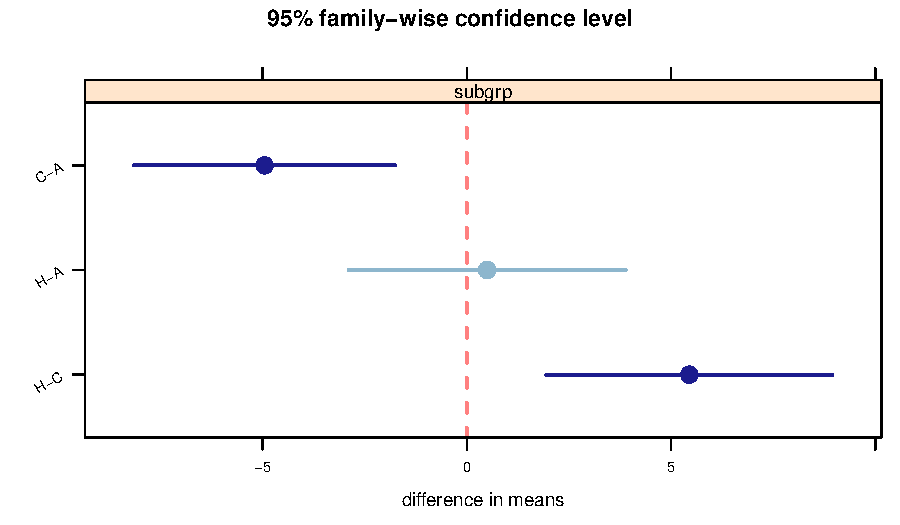
\includegraphics[width=\maxwidth]{figures/FrontMatter-help-hsd3-1} 

}



\end{knitrout}

Again, we see that the cocaine group has significantly lower CESD scores
than either of the other two groups.

\chapter{Categorical Response, Quantitative Predictor}


\section{Logistic regression}
\myindex{logistic regression}%

Logistic regression is available using the \function{glm()} function, 
which supports
a variety of
link functions and distributional forms for generalized linear models, including logistic regression.
\FoodForThought[-1cm]{The \function{glm()} function has argument \option{family}, which can take an option 
\option{link}.  The \code{logit} link is the default link for the binomial family,
so we don't need to specify it here. The more verbose usage would be \code{family=binomial(link=logit)}.}%
\Rindex{glm()}%
\Rindex{family option}%
\Rindex{exp()}%
\Rindex{msummary()}%
\begin{knitrout}\small
\definecolor{shadecolor}{rgb}{1, 1, 1}\color{fgcolor}\begin{kframe}
\begin{alltt}
\hlstd{> }\hlstd{logitmod} \hlkwb{<-} \hlkwd{glm}\hlstd{(homeless} \hlopt{~} \hlstd{age} \hlopt{+} \hlstd{female,} \hlkwc{family}\hlstd{=binomial,}
\hlstd{ }  \hlkwc{data}\hlstd{=HELPrct)}
\hlstd{> }\hlkwd{msummary}\hlstd{(logitmod)}
\end{alltt}
\begin{verbatim}
Coefficients:
            Estimate Std. Error z value Pr(>|z|)
(Intercept)   0.8926     0.4537    1.97    0.049
age          -0.0239     0.0124   -1.92    0.055
female        0.4920     0.2282    2.16    0.031

(Dispersion parameter for binomial family taken to be 1)

    Null deviance: 625.28  on 452  degrees of freedom
Residual deviance: 617.19  on 450  degrees of freedom
AIC: 623.2

Number of Fisher Scoring iterations: 4
\end{verbatim}
\begin{alltt}
\hlstd{> }\hlkwd{exp}\hlstd{(}\hlkwd{coef}\hlstd{(logitmod))}
\end{alltt}
\begin{verbatim}
(Intercept)         age      female 
     2.4415      0.9764      1.6355 
\end{verbatim}
\begin{alltt}
\hlstd{> }\hlkwd{exp}\hlstd{(}\hlkwd{confint}\hlstd{(logitmod))}
\end{alltt}


{\ttfamily\noindent\itshape\color{messagecolor}{Waiting for profiling to be done...}}\begin{verbatim}
             2.5 % 97.5 %
(Intercept) 1.0081  5.988
age         0.9527  1.000
female      1.0501  2.574
\end{verbatim}
\end{kframe}
\end{knitrout}

We can compare two models (for multiple degree of freedom tests).  For example, we
might be interested in the association of homeless status and age for each of the three substance groups.
\Rindex{anova()}%
\Rindex{test option}%
\begin{knitrout}\small
\definecolor{shadecolor}{rgb}{1, 1, 1}\color{fgcolor}\begin{kframe}
\begin{alltt}
\hlstd{> }\hlstd{mymodsubage} \hlkwb{<-} \hlkwd{glm}\hlstd{((homeless}\hlopt{==}\hlstr{"homeless"}\hlstd{)} \hlopt{~} \hlstd{age} \hlopt{+} \hlstd{substance,}
\hlstd{ }  \hlkwc{family}\hlstd{=binomial,} \hlkwc{data}\hlstd{=HELPrct)}
\hlstd{> }\hlstd{mymodage} \hlkwb{<-} \hlkwd{glm}\hlstd{((homeless}\hlopt{==}\hlstr{"homeless"}\hlstd{)} \hlopt{~} \hlstd{age,} \hlkwc{family}\hlstd{=binomial,}
\hlstd{ }  \hlkwc{data}\hlstd{=HELPrct)}
\hlstd{> }\hlkwd{msummary}\hlstd{(mymodsubage)}
\end{alltt}
\begin{verbatim}
Coefficients:
                 Estimate Std. Error z value Pr(>|z|)
(Intercept)       -0.0509     0.5164   -0.10   0.9215
age                0.0100     0.0129    0.77   0.4399
substancecocaine  -0.7496     0.2303   -3.25   0.0011
substanceheroin   -0.7780     0.2469   -3.15   0.0016

(Dispersion parameter for binomial family taken to be 1)

    Null deviance: 625.28  on 452  degrees of freedom
Residual deviance: 607.62  on 449  degrees of freedom
AIC: 615.6

Number of Fisher Scoring iterations: 4
\end{verbatim}
\begin{alltt}
\hlstd{> }\hlkwd{exp}\hlstd{(}\hlkwd{coef}\hlstd{(mymodsubage))}
\end{alltt}
\begin{verbatim}
     (Intercept)              age substancecocaine  substanceheroin 
          0.9504           1.0101           0.4725           0.4593 
\end{verbatim}
\begin{alltt}
\hlstd{> }\hlkwd{anova}\hlstd{(mymodage, mymodsubage,} \hlkwc{test}\hlstd{=}\hlstr{"Chisq"}\hlstd{)}
\end{alltt}
\begin{verbatim}
Analysis of Deviance Table

Model 1: (homeless == "homeless") ~ age
Model 2: (homeless == "homeless") ~ age + substance
  Resid. Df Resid. Dev Df Deviance Pr(>Chi)
1       451        622                     
2       449        608  2     14.3  0.00078
\end{verbatim}
\end{kframe}
\end{knitrout}
We observe that the cocaine and heroin groups are significantly less likely to be homeless than alcohol involved subjects, after controlling for age.  (A similar result is seen when considering just homeless status and substance.)

\begin{knitrout}\small
\definecolor{shadecolor}{rgb}{1, 1, 1}\color{fgcolor}\begin{kframe}
\begin{alltt}
\hlstd{> }\hlkwd{tally}\hlstd{(}\hlopt{~} \hlstd{homeless} \hlopt{|} \hlstd{substance,} \hlkwc{format}\hlstd{=}\hlstr{"percent"}\hlstd{,} \hlkwc{margins}\hlstd{=}\hlnum{TRUE}\hlstd{,} \hlkwc{data}\hlstd{=HELPrct)}
\end{alltt}
\begin{verbatim}
          substance
homeless   alcohol cocaine heroin
  homeless   58.19   38.82  37.90
  housed     41.81   61.18  62.10
  Total     100.00  100.00 100.00
\end{verbatim}
\end{kframe}
\end{knitrout}



\chapter{Survival Time Outcomes}

\myindex{survival analysis}%
\myindex{failure time analysis}%
\myindex{time to event analysis}%
Extensive support for survival (time to event) analysis is available within the 
\pkg{survival} package.

\section{Kaplan-Meier plot}

\myindex{Kaplan-Meier plot}%
\Rindex{survfit()}%
\Rindex{Surv()}%
\Rindex{conf.int option}%
\Rindex{xlab option}%
\begin{center}
\begin{knitrout}\small
\definecolor{shadecolor}{rgb}{1, 1, 1}\color{fgcolor}\begin{kframe}
\begin{alltt}
\hlstd{> }\hlkwd{require}\hlstd{(survival)}
\hlstd{> }\hlstd{fit} \hlkwb{<-} \hlkwd{survfit}\hlstd{(}\hlkwd{Surv}\hlstd{(dayslink, linkstatus)} \hlopt{~} \hlstd{treat,}
\hlstd{ }  \hlkwc{data}\hlstd{=HELPrct)}
\hlstd{> }\hlkwd{plot}\hlstd{(fit,} \hlkwc{conf.int}\hlstd{=}\hlnum{FALSE}\hlstd{,} \hlkwc{lty}\hlstd{=}\hlnum{1}\hlopt{:}\hlnum{2}\hlstd{,} \hlkwc{lwd}\hlstd{=}\hlnum{2}\hlstd{,}
\hlstd{ }  \hlkwc{xlab}\hlstd{=}\hlstr{"time (in days)"}\hlstd{,} \hlkwc{ylab}\hlstd{=}\hlstr{"P(not linked)"}\hlstd{)}
\hlstd{> }\hlkwd{legend}\hlstd{(}\hlnum{20}\hlstd{,} \hlnum{0.4}\hlstd{,} \hlkwc{legend}\hlstd{=}\hlkwd{c}\hlstd{(}\hlstr{"Control"}\hlstd{,} \hlstr{"Treatment"}\hlstd{),}
\hlstd{ }  \hlkwc{lty}\hlstd{=}\hlkwd{c}\hlstd{(}\hlnum{1}\hlstd{,}\hlnum{2}\hlstd{),} \hlkwc{lwd}\hlstd{=}\hlnum{2}\hlstd{)}
\hlstd{> }\hlkwd{title}\hlstd{(}\hlstr{"Product-Limit Survival Estimates (time to linkage)"}\hlstd{)}
\end{alltt}
\end{kframe}

{\centering 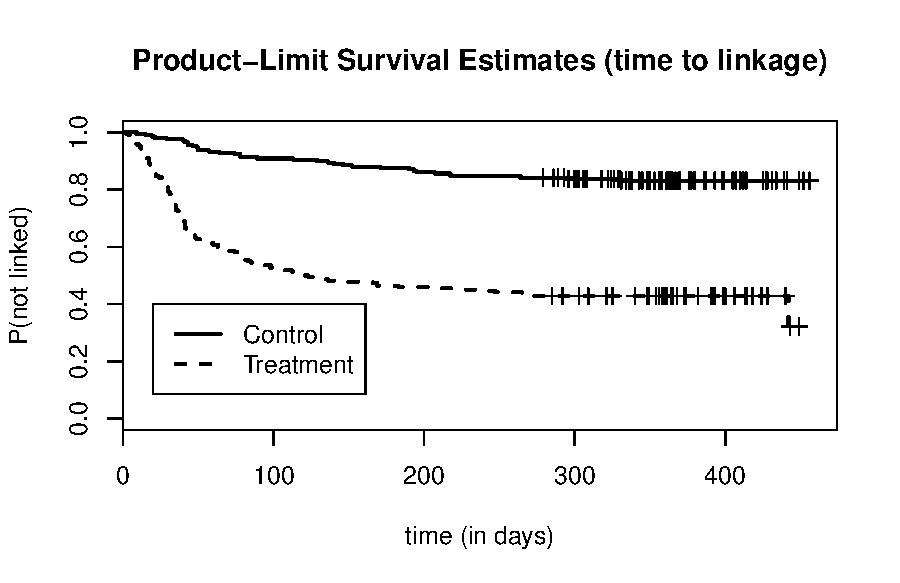
\includegraphics[width=\maxwidth]{figures/FrontMatter-help-km-1} 

}



\end{knitrout}
\end{center}

We see that the subjects in the treatment (Health Evaluation and Linkage to Primary Care clinic) were significantly more likely to 
link to primary care (less likely to ``survive'') than the control (usual care) group.

\section{Cox proportional hazards model}
\myindex{Cox proportional hazards model}%
\myindex{proportional hazards model}%
\Rindex{coxph()}%

\begin{knitrout}\small
\definecolor{shadecolor}{rgb}{1, 1, 1}\color{fgcolor}\begin{kframe}
\begin{alltt}
\hlstd{> }\hlkwd{require}\hlstd{(survival)}
\hlstd{> }\hlkwd{summary}\hlstd{(}\hlkwd{coxph}\hlstd{(}\hlkwd{Surv}\hlstd{(dayslink, linkstatus)} \hlopt{~} \hlstd{age} \hlopt{+} \hlstd{substance,}
\hlstd{ }  \hlkwc{data}\hlstd{=HELPrct))}
\end{alltt}
\begin{verbatim}
Call:
coxph(formula = Surv(dayslink, linkstatus) ~ age + substance, 
    data = HELPrct)

  n= 431, number of events= 163 
   (22 observations deleted due to missingness)

                     coef exp(coef) se(coef)     z Pr(>|z|)
age               0.00893   1.00897  0.01026  0.87     0.38
substancecocaine  0.18045   1.19775  0.18100  1.00     0.32
substanceheroin  -0.28970   0.74849  0.21725 -1.33     0.18

                 exp(coef) exp(-coef) lower .95 upper .95
age                  1.009      0.991     0.989      1.03
substancecocaine     1.198      0.835     0.840      1.71
substanceheroin      0.748      1.336     0.489      1.15

Concordance= 0.55  (se = 0.023 )
Rsquare= 0.014   (max possible= 0.988 )
Likelihood ratio test= 6.11  on 3 df,   p=0.106
Wald test            = 5.84  on 3 df,   p=0.12
Score (logrank) test = 5.91  on 3 df,   p=0.116
\end{verbatim}
\end{kframe}
\end{knitrout}

Neither age nor substance group was significantly associated with linkage to primary care.


\chapter{More than Two Variables}


\section{Two (or more) way ANOVA}

We can fit a two (or more) way ANOVA model, without or with an interaction,
using the same modeling syntax.
\Rindex{median()}%
\Rindex{bwplot()}%
\Rindex{factor()}%
\Rindex{mutate()}%
\Rindex{aov()}%
\begin{knitrout}\small
\definecolor{shadecolor}{rgb}{1, 1, 1}\color{fgcolor}\begin{kframe}
\begin{alltt}
\hlstd{> }\hlstd{HELPrct} \hlkwb{<-} \hlkwd{mutate}\hlstd{(HELPrct,} \hlkwc{subgrp} \hlstd{=} \hlkwd{factor}\hlstd{(substance,}
\hlstd{ }  \hlkwc{levels}\hlstd{=}\hlkwd{c}\hlstd{(}\hlstr{"alcohol"}\hlstd{,} \hlstr{"cocaine"}\hlstd{,} \hlstr{"heroin"}\hlstd{),}
\hlstd{ }  \hlkwc{labels}\hlstd{=}\hlkwd{c}\hlstd{(}\hlstr{"A"}\hlstd{,} \hlstr{"C"}\hlstd{,} \hlstr{"H"}\hlstd{)))}
\hlstd{> }\hlkwd{median}\hlstd{(cesd} \hlopt{~} \hlstd{substance} \hlopt{|} \hlstd{sex,} \hlkwc{data}\hlstd{=HELPrct)}
\end{alltt}
\begin{verbatim}
alcohol.female cocaine.female  heroin.female   alcohol.male 
          40.0           35.0           39.0           33.0 
  cocaine.male    heroin.male         female           male 
          29.0           34.5           38.0           32.5 
\end{verbatim}
\begin{alltt}
\hlstd{> }\hlkwd{bwplot}\hlstd{(cesd} \hlopt{~} \hlstd{subgrp} \hlopt{|} \hlstd{sex,} \hlkwc{data}\hlstd{=HELPrct)}
\end{alltt}
\end{kframe}

{\centering 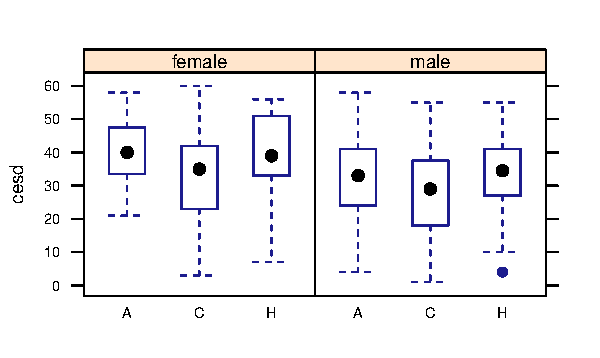
\includegraphics[width=\maxwidth]{figures/FrontMatter-help-aovplot-1} 

}



\end{knitrout}
\begin{knitrout}\small
\definecolor{shadecolor}{rgb}{1, 1, 1}\color{fgcolor}\begin{kframe}
\begin{alltt}
\hlstd{> }\hlkwd{summary}\hlstd{(}\hlkwd{aov}\hlstd{(cesd} \hlopt{~} \hlstd{substance} \hlopt{+} \hlstd{sex,} \hlkwc{data}\hlstd{=HELPrct))}
\end{alltt}
\begin{verbatim}
             Df Sum Sq Mean Sq F value  Pr(>F)
substance     2   2704    1352    9.27 0.00011
sex           1   2569    2569   17.61 3.3e-05
Residuals   449  65515     146                
\end{verbatim}
\end{kframe}
\end{knitrout}
\begin{knitrout}\small
\definecolor{shadecolor}{rgb}{1, 1, 1}\color{fgcolor}\begin{kframe}
\begin{alltt}
\hlstd{> }\hlkwd{summary}\hlstd{(}\hlkwd{aov}\hlstd{(cesd} \hlopt{~} \hlstd{substance} \hlopt{*} \hlstd{sex,} \hlkwc{data}\hlstd{=HELPrct))}
\end{alltt}
\begin{verbatim}
               Df Sum Sq Mean Sq F value  Pr(>F)
substance       2   2704    1352    9.25 0.00012
sex             1   2569    2569   17.57 3.3e-05
substance:sex   2    146      73    0.50 0.60752
Residuals     447  65369     146                
\end{verbatim}
\end{kframe}
\end{knitrout}
There's little evidence for the interaction, though there are statistically
significant main effects terms for \variable{substance} group and 
\variable{sex}.

\begin{knitrout}\small
\definecolor{shadecolor}{rgb}{1, 1, 1}\color{fgcolor}\begin{kframe}
\begin{alltt}
\hlstd{> }\hlkwd{xyplot}\hlstd{(cesd} \hlopt{~} \hlstd{substance,} \hlkwc{groups}\hlstd{=sex,} \hlkwc{lwd}\hlstd{=}\hlnum{2}\hlstd{,}
\hlstd{ }  \hlkwc{auto.key}\hlstd{=}\hlkwd{list}\hlstd{(}\hlkwc{columns}\hlstd{=}\hlnum{2}\hlstd{,} \hlkwc{lines}\hlstd{=}\hlnum{TRUE}\hlstd{,} \hlkwc{points}\hlstd{=}\hlnum{FALSE}\hlstd{),}
\hlstd{ }  \hlkwc{type}\hlstd{=}\hlstr{'a'}\hlstd{,} \hlkwc{data}\hlstd{=HELPrct)}
\end{alltt}
\end{kframe}

{\centering 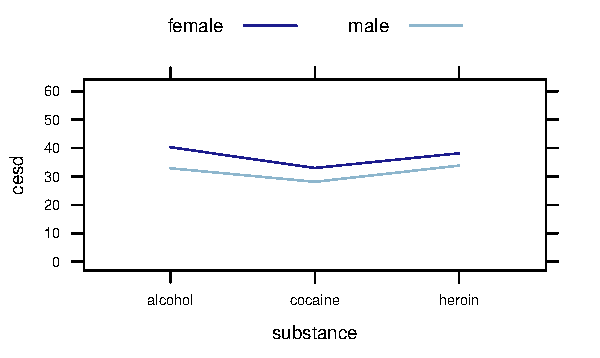
\includegraphics[width=\maxwidth]{figures/FrontMatter-help-interaction-1} 

}



\end{knitrout}
\Rindex{auto.key option}%


\section{Multiple regression}
\myindex{multiple regression}%
\myindex{multivariate relationships}%

Multiple regression is a logical extension of the prior commands, where 
additional predictors are added.  This allows students to start to try to disentangle 
multivariate relationships.  

\InstructorNote[-2cm]{We tend to introduce multiple linear regression
early in our courses, as a purely descriptive technique, then return to it
regularly.  The motivation for this is described at length in the companion volume 
\emph{Start Modeling with R}.}

Here we consider a model (parallel slopes) for depressive symptoms as a function of Mental Component Score (MCS),
age (in years) and sex of the subject.

\myindex{msummary()}%
\begin{knitrout}\small
\definecolor{shadecolor}{rgb}{1, 1, 1}\color{fgcolor}\begin{kframe}
\begin{alltt}
\hlstd{> }\hlstd{lmnointeract} \hlkwb{<-} \hlkwd{lm}\hlstd{(cesd} \hlopt{~} \hlstd{mcs} \hlopt{+} \hlstd{age} \hlopt{+} \hlstd{sex,} \hlkwc{data}\hlstd{=HELPrct)}
\hlstd{> }\hlkwd{msummary}\hlstd{(lmnointeract)}
\end{alltt}
\begin{verbatim}
            Estimate Std. Error t value Pr(>|t|)
(Intercept)  53.8303     2.3617   22.79   <2e-16
mcs          -0.6548     0.0336  -19.50   <2e-16
age           0.0553     0.0556    1.00   0.3200
sexmale      -2.8993     1.0137   -2.86   0.0044

Residual standard error: 9.09 on 449 degrees of freedom
Multiple R-squared:  0.476,	Adjusted R-squared:  0.473 
F-statistic:  136 on 3 and 449 DF,  p-value: <2e-16
\end{verbatim}
\end{kframe}
\end{knitrout}
\myindex{anova()}%
\myindex{interactions}%
We can also fit a model that includes an interaction between MCS and sex.
\begin{knitrout}\small
\definecolor{shadecolor}{rgb}{1, 1, 1}\color{fgcolor}\begin{kframe}
\begin{alltt}
\hlstd{> }\hlstd{lminteract} \hlkwb{<-} \hlkwd{lm}\hlstd{(cesd} \hlopt{~} \hlstd{mcs} \hlopt{+} \hlstd{age} \hlopt{+} \hlstd{sex} \hlopt{+} \hlstd{mcs}\hlopt{:}\hlstd{sex,} \hlkwc{data}\hlstd{=HELPrct)}
\hlstd{> }\hlkwd{msummary}\hlstd{(lminteract)}
\end{alltt}
\begin{verbatim}
            Estimate Std. Error t value Pr(>|t|)
(Intercept)  55.3906     2.9903   18.52   <2e-16
mcs          -0.7082     0.0712   -9.95   <2e-16
age           0.0549     0.0556    0.99    0.324
sexmale      -4.9421     2.6055   -1.90    0.058
mcs:sexmale   0.0687     0.0807    0.85    0.395

Residual standard error: 9.09 on 448 degrees of freedom
Multiple R-squared:  0.477,	Adjusted R-squared:  0.472 
F-statistic:  102 on 4 and 448 DF,  p-value: <2e-16
\end{verbatim}
\begin{alltt}
\hlstd{> }\hlkwd{anova}\hlstd{(lminteract)}
\end{alltt}
\begin{verbatim}
Analysis of Variance Table

Response: cesd
           Df Sum Sq Mean Sq F value Pr(>F)
mcs         1  32918   32918  398.27 <2e-16
age         1    107     107    1.29 0.2563
sex         1    676     676    8.18 0.0044
mcs:sex     1     60      60    0.72 0.3952
Residuals 448  37028      83               
\end{verbatim}
\end{kframe}
\end{knitrout}
\begin{knitrout}\small
\definecolor{shadecolor}{rgb}{1, 1, 1}\color{fgcolor}\begin{kframe}
\begin{alltt}
\hlstd{> }\hlkwd{anova}\hlstd{(lmnointeract, lminteract)}
\end{alltt}
\begin{verbatim}
Analysis of Variance Table

Model 1: cesd ~ mcs + age + sex
Model 2: cesd ~ mcs + age + sex + mcs:sex
  Res.Df   RSS Df Sum of Sq    F Pr(>F)
1    449 37088                         
2    448 37028  1      59.9 0.72    0.4
\end{verbatim}
\end{kframe}
\end{knitrout}

There is little evidence for an interaction effect, so we drop
this from the model.

\subsection{Visualizing the results from the regression}

\label{sec:plotFun}
\Rindex{plotFun()}%
\Rindex{makeFun()}%
The \function{makeFun()} and \function{plotFun()} functions from the \pkg{mosaic} package 
can be used to display the predicted values from a regression model.  For this example, we might 
display the predicted CESD values for a range of MCS (mental component score) values a hypothetical 36 year old male and female subject might have from the parallel
slopes (no interaction) model.
\begin{knitrout}\small
\definecolor{shadecolor}{rgb}{1, 1, 1}\color{fgcolor}\begin{kframe}
\begin{alltt}
\hlstd{> }\hlstd{lmfunction} \hlkwb{<-} \hlkwd{makeFun}\hlstd{(lmnointeract)}
\end{alltt}
\end{kframe}
\end{knitrout}

\Rindex{xyplot()}%
\Rindex{auto.key option}%
\Rindex{ylab option}%
\Rindex{groups option}%
\Rindex{add option}%
We can now plot the predicted values separately for male and female subjects over a range of MCS (mental component score) values, along
with the observed data for all of the 36 year olds.  
\begin{knitrout}\small
\definecolor{shadecolor}{rgb}{1, 1, 1}\color{fgcolor}\begin{kframe}
\begin{alltt}
\hlstd{> }\hlkwd{xyplot}\hlstd{(cesd} \hlopt{~} \hlstd{mcs,} \hlkwc{groups}\hlstd{=sex,} \hlkwc{auto.key}\hlstd{=}\hlnum{TRUE}\hlstd{,}
\hlstd{ }  \hlkwc{data}\hlstd{=}\hlkwd{filter}\hlstd{(HELPrct, age}\hlopt{==}\hlnum{36}\hlstd{))}
\hlstd{> }\hlkwd{plotFun}\hlstd{(}\hlkwd{lmfunction}\hlstd{(mcs,} \hlkwc{age}\hlstd{=}\hlnum{36}\hlstd{,} \hlkwc{sex}\hlstd{=}\hlstr{"male"}\hlstd{)} \hlopt{~} \hlstd{mcs,}
\hlstd{ }  \hlkwc{xlim}\hlstd{=}\hlkwd{c}\hlstd{(}\hlnum{0}\hlstd{,} \hlnum{60}\hlstd{),} \hlkwc{lwd}\hlstd{=}\hlnum{2}\hlstd{,} \hlkwc{ylab}\hlstd{=}\hlstr{"predicted CESD"}\hlstd{,} \hlkwc{add}\hlstd{=}\hlnum{TRUE}\hlstd{)}
\hlstd{> }\hlkwd{plotFun}\hlstd{(}\hlkwd{lmfunction}\hlstd{(mcs,} \hlkwc{age}\hlstd{=}\hlnum{36}\hlstd{,} \hlkwc{sex}\hlstd{=}\hlstr{"female"}\hlstd{)} \hlopt{~} \hlstd{mcs,}
\hlstd{ }  \hlkwc{xlim}\hlstd{=}\hlkwd{c}\hlstd{(}\hlnum{0}\hlstd{,} \hlnum{60}\hlstd{),} \hlkwc{lty}\hlstd{=}\hlnum{2}\hlstd{,} \hlkwc{lwd}\hlstd{=}\hlnum{3}\hlstd{,} \hlkwc{add}\hlstd{=}\hlnum{TRUE}\hlstd{)}
\end{alltt}
\end{kframe}

{\centering 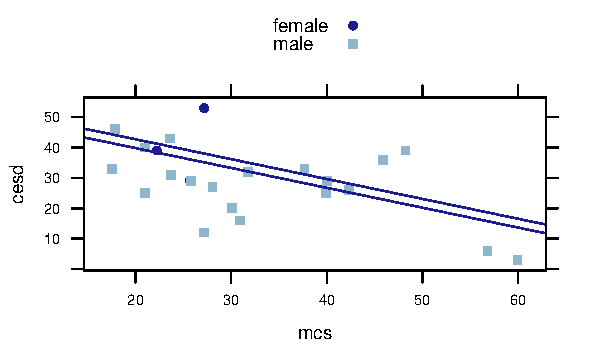
\includegraphics[width=\maxwidth]{figures/FrontMatter-plotFUN-1} 

}



\end{knitrout}


\subsection{Coefficient plots}

\myindex{coefficient plots}%
It is sometimes useful to display a plot of the coefficients for a multiple regression model (along with their associated
confidence intervals).

\Rindex{mplot()}%
\begin{knitrout}\small
\definecolor{shadecolor}{rgb}{1, 1, 1}\color{fgcolor}\begin{kframe}
\begin{alltt}
\hlstd{> }\hlkwd{mplot}\hlstd{(lmnointeract,} \hlkwc{rows}\hlstd{=}\hlopt{-}\hlnum{1}\hlstd{,} \hlkwc{which}\hlstd{=}\hlnum{7}\hlstd{)}
\end{alltt}
\end{kframe}

{\centering 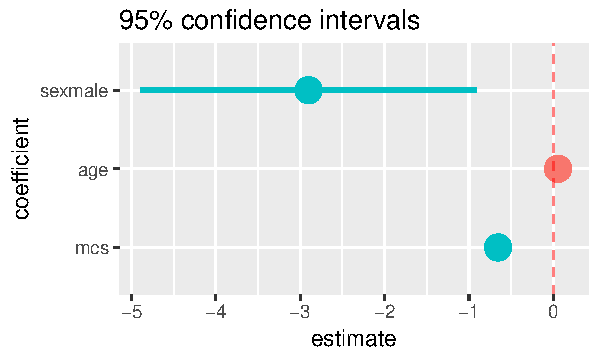
\includegraphics[width=\maxwidth]{figures/FrontMatter-unnamed-chunk-50-1} 

}



\end{knitrout}

\FoodForThought[-4cm]{Darker dots indicate regression coefficients where the 95\% confidence interval does not include the null hypothesis value of zero.}

\Caution{Be careful when fitting regression models with missing values (see also section \ref{sec:miss}).}

\subsection{Residual diagnostics}
\myindex{residual diagnostics}
\myindex{regression diagnostics}

It's straightforward to undertake residual diagnostics for this model.  We begin by adding the
fitted values and residuals to the dataset.
\FoodForThought[-1cm]{The \function{mplot} function can also be used to create these graphs.}
\Rindex{resid()}%
\Rindex{fitted()}%
\Rindex{abs()}%
\InstructorNote{Here we are adding two new variables into an existing dataset. It's often a good practice to give the resulting dataframe a new name.}
\begin{knitrout}\small
\definecolor{shadecolor}{rgb}{1, 1, 1}\color{fgcolor}\begin{kframe}
\begin{alltt}
\hlstd{> }\hlstd{HELPrct} \hlkwb{<-} \hlkwd{mutate}\hlstd{(HELPrct,}
\hlstd{ }  \hlkwc{residuals} \hlstd{=} \hlkwd{resid}\hlstd{(lmnointeract),}
\hlstd{ }  \hlkwc{pred} \hlstd{=} \hlkwd{fitted}\hlstd{(lmnointeract))}
\end{alltt}
\end{kframe}
\end{knitrout}
\begin{knitrout}\small
\definecolor{shadecolor}{rgb}{1, 1, 1}\color{fgcolor}\begin{kframe}
\begin{alltt}
\hlstd{> }\hlkwd{histogram}\hlstd{(}\hlopt{~} \hlstd{residuals,} \hlkwc{xlab}\hlstd{=}\hlstr{"residuals"}\hlstd{,} \hlkwc{fit}\hlstd{=}\hlstr{"normal"}\hlstd{,}
\hlstd{ }  \hlkwc{data}\hlstd{=HELPrct)}
\end{alltt}
\end{kframe}

{\centering 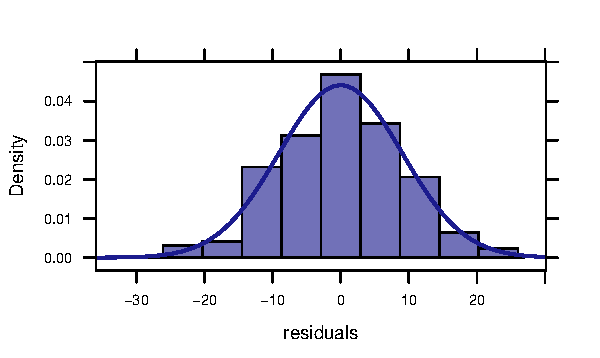
\includegraphics[width=\maxwidth]{figures/FrontMatter-unnamed-chunk-52-1} 

}



\end{knitrout}

We can identify the subset of observations with extremely large residuals.

\Rindex{abs()}%
\begin{knitrout}\small
\definecolor{shadecolor}{rgb}{1, 1, 1}\color{fgcolor}\begin{kframe}
\begin{alltt}
\hlstd{> }\hlkwd{filter}\hlstd{(HELPrct,} \hlkwd{abs}\hlstd{(residuals)} \hlopt{>} \hlnum{25}\hlstd{)}
\end{alltt}
\begin{verbatim}
  age anysubstatus anysub cesd d1 daysanysub dayslink drugrisk e2b
1  43            0     no   16 15        191      414        0  NA
2  27           NA   <NA>   40  1         NA      365        3   2
  female  sex g1b homeless i1 i2  id indtot linkstatus link   mcs
1      0 male  no homeless 24 36  44     41          0   no 15.86
2      0 male  no homeless 18 18 420     37          0   no 57.49
    pcs pss_fr racegrp satreat sexrisk substance treat subgrp
1 71.39      3   white      no       7   cocaine   yes      C
2 37.75      8   white     yes       3    heroin    no      H
  residuals  pred
1    -26.92 42.92
2     25.22 14.78
\end{verbatim}
\end{kframe}
\end{knitrout}

\Rindex{cex option}%
\Rindex{type option}%
\begin{knitrout}\small
\definecolor{shadecolor}{rgb}{1, 1, 1}\color{fgcolor}\begin{kframe}
\begin{alltt}
\hlstd{> }\hlkwd{xyplot}\hlstd{(residuals} \hlopt{~} \hlstd{pred,} \hlkwc{ylab}\hlstd{=}\hlstr{"residuals"}\hlstd{,} \hlkwc{cex}\hlstd{=}\hlnum{0.3}\hlstd{,}
\hlstd{ }  \hlkwc{xlab}\hlstd{=}\hlstr{"predicted values"}\hlstd{,} \hlkwc{main}\hlstd{=}\hlstr{"predicted vs. residuals"}\hlstd{,}
\hlstd{ }  \hlkwc{type}\hlstd{=}\hlkwd{c}\hlstd{(}\hlstr{"p"}\hlstd{,} \hlstr{"r"}\hlstd{,} \hlstr{"smooth"}\hlstd{),} \hlkwc{data}\hlstd{=HELPrct)}
\end{alltt}
\end{kframe}

{\centering 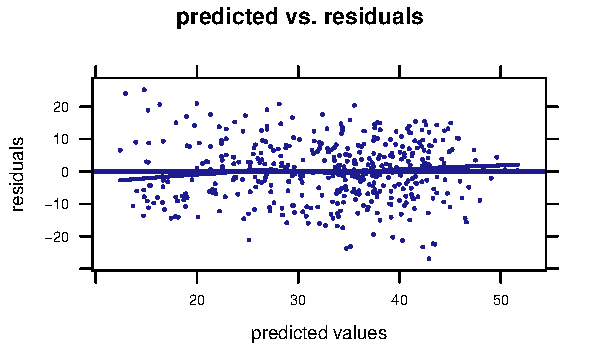
\includegraphics[width=\maxwidth]{figures/FrontMatter-unnamed-chunk-54-1} 

}



\end{knitrout}
\begin{knitrout}\small
\definecolor{shadecolor}{rgb}{1, 1, 1}\color{fgcolor}\begin{kframe}
\begin{alltt}
\hlstd{> }\hlkwd{xyplot}\hlstd{(residuals} \hlopt{~} \hlstd{mcs,} \hlkwc{xlab}\hlstd{=}\hlstr{"mental component score"}\hlstd{,}
\hlstd{ }  \hlkwc{ylab}\hlstd{=}\hlstr{"residuals"}\hlstd{,} \hlkwc{cex}\hlstd{=}\hlnum{0.3}\hlstd{,}
\hlstd{ }  \hlkwc{type}\hlstd{=}\hlkwd{c}\hlstd{(}\hlstr{"p"}\hlstd{,} \hlstr{"r"}\hlstd{,} \hlstr{"smooth"}\hlstd{),} \hlkwc{data}\hlstd{=HELPrct)}
\end{alltt}
\end{kframe}

{\centering 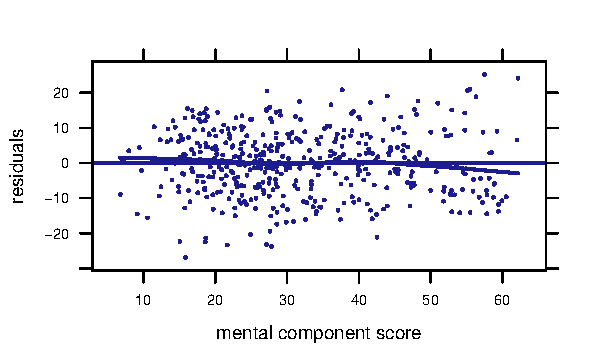
\includegraphics[width=\maxwidth]{figures/FrontMatter-unnamed-chunk-55-1} 

}



\end{knitrout}

The assumptions of normality, linearity and homoscedasticity seem reasonable here.
\begin{problem}
The \dataframe{RailTrail} dataset within the \pkg{mosaic} package includes the counts 
of crossings of a rail trail in Northampton, Massachusetts for 90 days in 2005.  
City officials are interested in understanding usage of the trail network, and
how it changes as a function of temperature and day of the week.  
Describe the distribution of the variable \variable{avgtemp} in terms of its
center, spread and shape.
\begin{knitrout}\small
\definecolor{shadecolor}{rgb}{1, 1, 1}\color{fgcolor}\begin{kframe}
\begin{alltt}
\hlstd{> }\hlkwd{favstats}\hlstd{(}\hlopt{~} \hlstd{avgtemp,} \hlkwc{data}\hlstd{=RailTrail)}
\end{alltt}
\begin{verbatim}
 min    Q1 median   Q3 max  mean    sd  n missing
  33 48.62  55.25 64.5  84 57.43 11.33 90       0
\end{verbatim}
\begin{alltt}
\hlstd{> }\hlkwd{densityplot}\hlstd{(}\hlopt{~} \hlstd{avgtemp,} \hlkwc{xlab}\hlstd{=}\hlstr{"Average daily temp (degrees F)"}\hlstd{,}
\hlstd{ }  \hlkwc{data}\hlstd{=RailTrail)}
\end{alltt}
\end{kframe}

{\centering 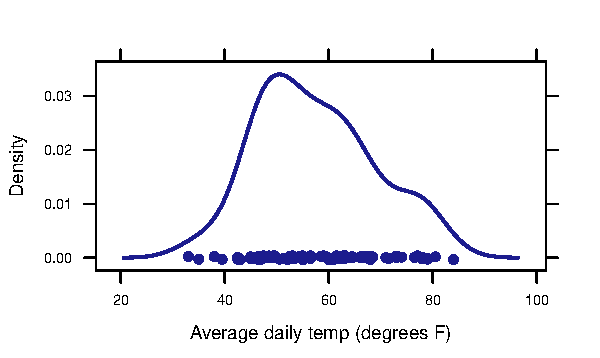
\includegraphics[width=\maxwidth]{figures/FrontMatter-unnamed-chunk-56-1} 

}



\end{knitrout}
\end{problem}
\begin{solution}
The distribution of average temperature (in degrees Fahrenheit) is approximately normally
distributed with mean 57.4 degrees and standard deviation of 11.3 degrees.
\end{solution}
\begin{problem}
The \dataframe{RailTrail} dataset also includes a variable called \variable{cloudcover}.  
Describe the distribution of this variable in terms of its
center, spread and shape.
\end{problem}
\begin{solution}
\begin{knitrout}\small
\definecolor{shadecolor}{rgb}{1, 1, 1}\color{fgcolor}\begin{kframe}
\begin{alltt}
\hlstd{> }\hlkwd{favstats}\hlstd{(}\hlopt{~} \hlstd{cloudcover,} \hlkwc{data}\hlstd{=RailTrail)}
\end{alltt}
\begin{verbatim}
 min   Q1 median    Q3 max  mean    sd  n missing
   0 3.65    6.4 8.475  10 5.807 3.226 90       0
\end{verbatim}
\begin{alltt}
\hlstd{> }\hlkwd{densityplot}\hlstd{(}\hlopt{~} \hlstd{cloudcover,} \hlkwc{data}\hlstd{=RailTrail)}
\end{alltt}
\end{kframe}

{\centering 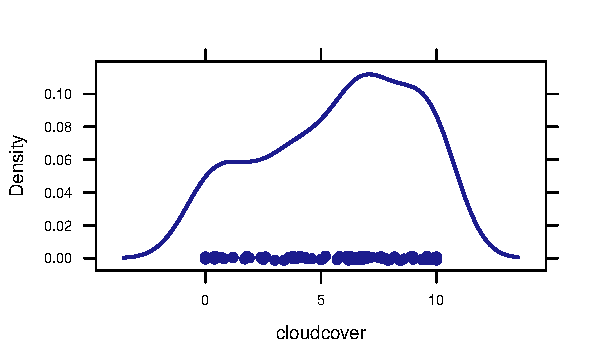
\includegraphics[width=\maxwidth]{figures/FrontMatter-unnamed-chunk-57-1} 

}



\end{knitrout}
The distribution of cloud cover is ungainly (almost triangular), with increasing probability for more
cloudcover.  The mean is 5.8 oktas (out of 10), with standard deviation of 3.2 oktas.  It tends to be
cloudy in Northampton!
\end{solution}
\begin{problem}
The variable in the \dataframe{RailTrail} dataset that provides the daily count
of crossings is called \variable{volume}. 
Describe the distribution of this variable in terms of its
center, spread and shape.
\end{problem}
\begin{solution}
\begin{knitrout}\small
\definecolor{shadecolor}{rgb}{1, 1, 1}\color{fgcolor}\begin{kframe}
\begin{alltt}
\hlstd{> }\hlkwd{favstats}\hlstd{(}\hlopt{~} \hlstd{volume,} \hlkwc{data}\hlstd{=RailTrail)}
\end{alltt}
\begin{verbatim}
 min    Q1 median    Q3 max  mean    sd  n missing
 129 291.5    373 451.2 736 375.4 127.5 90       0
\end{verbatim}
\begin{alltt}
\hlstd{> }\hlkwd{densityplot}\hlstd{(}\hlopt{~} \hlstd{volume,} \hlkwc{xlab}\hlstd{=}\hlstr{"# of crossings"}\hlstd{,} \hlkwc{data}\hlstd{=RailTrail)}
\hlstd{> }\hlkwd{filter}\hlstd{(RailTrail, volume} \hlopt{>} \hlnum{700}\hlstd{)}
\end{alltt}
\begin{verbatim}
  hightemp lowtemp avgtemp spring summer fall cloudcover precip
1       77      52    64.5      1      0    0          5      0
  volume weekday
1    736       0
\end{verbatim}
\end{kframe}

{\centering \includegraphics[width=\maxwidth]{figures/FrontMatter-unnamed-chunk-58-1} 

}



\end{knitrout}
The distribution of daily crossings is approximately normally
distributed with mean 375 crossings  and standard deviation of 127 crossings.
There is one outlier with 736 crossings which occurred on a Monday holiday in the spring
(Memorial Day).  
\end{solution}
\begin{problem}
The \dataframe{RailTrail} dataset also contains an indicator of whether the day was 
a weekday (\variable{weekday==1}) or a weekend/holiday (\variable{weekday==0}).
Use \function{tally()} to describe the distribution of this categorical variable.
What percentage of the days are weekends/holidays?
\end{problem}
\begin{solution}
\begin{knitrout}\small
\definecolor{shadecolor}{rgb}{1, 1, 1}\color{fgcolor}\begin{kframe}
\begin{alltt}
\hlstd{> }\hlkwd{tally}\hlstd{(}\hlopt{~} \hlstd{weekday,} \hlkwc{data}\hlstd{=RailTrail)}
\end{alltt}
\begin{verbatim}
weekday
 0  1 
28 62 
\end{verbatim}
\begin{alltt}
\hlstd{> }\hlkwd{tally}\hlstd{(}\hlopt{~} \hlstd{weekday,} \hlkwc{format}\hlstd{=}\hlstr{"percent"}\hlstd{,} \hlkwc{data}\hlstd{=RailTrail)}
\end{alltt}
\begin{verbatim}
weekday
    0     1 
31.11 68.89 
\end{verbatim}
\end{kframe}
\end{knitrout}
Just over 30\% of the days are weekends or holidays.
\end{solution}
\begin{problem}
Use side-by-side boxplots to compare the distribution of \variable{volume} by day type in the \dataframe{RailTrail} dataset.
Hint: you'll need to turn the numeric \variable{weekday} variable into a factor variable using \function{as.factor()} or use the {\tt horizontal=FALSE} option.
What do you conclude?
\end{problem}
\begin{solution}
\begin{knitrout}\small
\definecolor{shadecolor}{rgb}{1, 1, 1}\color{fgcolor}\begin{kframe}
\begin{alltt}
\hlstd{> }\hlkwd{bwplot}\hlstd{(volume} \hlopt{~} \hlkwd{as.factor}\hlstd{(weekday),} \hlkwc{data}\hlstd{=RailTrail)}
\end{alltt}
\end{kframe}

{\centering \includegraphics[width=\maxwidth]{figures/FrontMatter-unnamed-chunk-60-1} 

}



\end{knitrout}
or
\begin{knitrout}\small
\definecolor{shadecolor}{rgb}{1, 1, 1}\color{fgcolor}\begin{kframe}
\begin{alltt}
\hlstd{> }\hlstd{RailTrail} \hlkwb{<-} \hlkwd{mutate}\hlstd{(RailTrail,} \hlkwc{daytype} \hlstd{=} \hlkwd{ifelse}\hlstd{(weekday}\hlopt{==}\hlnum{1}\hlstd{,} \hlstr{"weekday"}\hlstd{,} \hlstr{"weekend/holiday"}\hlstd{))}
\hlstd{> }\hlkwd{bwplot}\hlstd{(volume} \hlopt{~} \hlstd{daytype,} \hlkwc{data}\hlstd{=RailTrail)}
\end{alltt}
\end{kframe}

{\centering \includegraphics[width=\maxwidth]{figures/FrontMatter-unnamed-chunk-61-1} 

}



\end{knitrout}
We see that the weekend/holidays tend to have more users.
\end{solution}

\begin{problem}
Use overlapping densityplots to compare the distribution of \variable{volume} by day type in the 
\dataframe{RailTrail} dataset.
What do you conclude?
\end{problem}
\begin{solution}
\begin{knitrout}\small
\definecolor{shadecolor}{rgb}{1, 1, 1}\color{fgcolor}\begin{kframe}
\begin{alltt}
\hlstd{> }\hlkwd{densityplot}\hlstd{(volume} \hlopt{~} \hlstd{weekday,} \hlkwc{auto.key}\hlstd{=}\hlnum{TRUE}\hlstd{,} \hlkwc{data}\hlstd{=RailTrail)}
\end{alltt}
\end{kframe}

{\centering \includegraphics[width=\maxwidth]{figures/FrontMatter-unnamed-chunk-62-1} 

}



\end{knitrout}
We see that the weekend/holidays tend to have more users.
\end{solution}
\begin{problem}
Create a scatterplot of \variable{volume} as a function of \variable{avgtemp} using the \dataframe{RailTrail} dataset, along with a regression line and scatterplot
smoother (lowess curve).  What do you observe about the relationship?  
\end{problem}
\begin{solution}
\begin{knitrout}\small
\definecolor{shadecolor}{rgb}{1, 1, 1}\color{fgcolor}\begin{kframe}
\begin{alltt}
\hlstd{> }\hlkwd{xyplot}\hlstd{(volume} \hlopt{~} \hlstd{avgtemp,} \hlkwc{xlab}\hlstd{=}\hlstr{"average temperature (degrees F)"}\hlstd{,}
\hlstd{ }  \hlkwc{type}\hlstd{=}\hlkwd{c}\hlstd{(}\hlstr{"p"}\hlstd{,} \hlstr{"r"}\hlstd{,} \hlstr{"smooth"}\hlstd{),} \hlkwc{lwd}\hlstd{=}\hlnum{2}\hlstd{,} \hlkwc{data}\hlstd{=RailTrail)}
\end{alltt}
\end{kframe}

{\centering \includegraphics[width=\maxwidth]{figures/FrontMatter-unnamed-chunk-63-1} 

}



\end{knitrout}
We see that there is a positive relationship between these two variables, but the association is 
somewhat nonlinear (which makes sense as we wouldn't continue to predict an increase in usage when the 
temperature becomes uncomfortably warm).  
\end{solution}
\begin{problem}
Using the \dataframe{RailTrail} dataset,
fit a multiple regression model for \variable{volume} as a function of \variable{cloudcover}, \variable{avgtemp}, 
\variable{weekday} and the interaction
between day type and average temperature.
Is there evidence to retain the interaction term at the $\alpha=0.05$ level?
\end{problem}
\begin{solution}
\begin{knitrout}\small
\definecolor{shadecolor}{rgb}{1, 1, 1}\color{fgcolor}\begin{kframe}
\begin{alltt}
\hlstd{> }\hlstd{fm} \hlkwb{<-} \hlkwd{lm}\hlstd{(volume} \hlopt{~} \hlstd{cloudcover} \hlopt{+} \hlstd{avgtemp} \hlopt{+} \hlstd{weekday} \hlopt{+} \hlstd{avgtemp}\hlopt{:}\hlstd{weekday,} \hlkwc{data}\hlstd{=RailTrail)}
\hlstd{> }\hlkwd{summary}\hlstd{(fm)}
\end{alltt}
\begin{verbatim}

Call:
lm(formula = volume ~ cloudcover + avgtemp + weekday + avgtemp:weekday, 
    data = RailTrail)

Residuals:
    Min      1Q  Median      3Q     Max 
-208.73  -53.33    6.22   61.65  293.98 

Coefficients:
                 Estimate Std. Error t value Pr(>|t|)
(Intercept)        378.83      92.53    4.09  9.6e-05
cloudcover         -17.20       3.33   -5.16  1.6e-06
avgtemp              2.31       1.51    1.53   0.1288
weekday1          -321.12     113.10   -2.84   0.0057
avgtemp:weekday1     4.73       1.92    2.47   0.0157

Residual standard error: 97.4 on 85 degrees of freedom
Multiple R-squared:  0.442,	Adjusted R-squared:  0.416 
F-statistic: 16.8 on 4 and 85 DF,  p-value: 3.34e-10
\end{verbatim}
\end{kframe}
\end{knitrout}
The interaction between average temperature and day-type is statistically significant (p=0.016).  We 
interpret this as being a steeper slope (stronger association) on weekdays rather than weekends.
(Perhaps on weekends/holidays people will tend to head out on the trails irrespective of the weather?)
\end{solution}
\begin{problem}
Use \function{makeFun()} to calculate the predicted number of crossings on a weekday with average 
temperature 60 degrees and no clouds.  Verify this calculation using the coefficients from the 
model.
\begin{knitrout}\small
\definecolor{shadecolor}{rgb}{1, 1, 1}\color{fgcolor}\begin{kframe}
\begin{alltt}
\hlstd{> }\hlkwd{coef}\hlstd{(fm)}
\end{alltt}
\begin{verbatim}
     (Intercept)       cloudcover          avgtemp         weekday1 
         378.834          -17.198            2.313         -321.116 
avgtemp:weekday1 
           4.727 
\end{verbatim}
\end{kframe}
\end{knitrout}
\end{problem}
\begin{solution}
\begin{knitrout}\small
\definecolor{shadecolor}{rgb}{1, 1, 1}\color{fgcolor}\begin{kframe}
\begin{alltt}
\hlstd{> }\hlstd{myfun} \hlkwb{<-} \hlkwd{makeFun}\hlstd{(fm)}
\hlstd{> }\hlkwd{myfun}\hlstd{(}\hlkwc{cloudcover}\hlstd{=}\hlnum{0}\hlstd{,} \hlkwc{avgtemp}\hlstd{=}\hlnum{60}\hlstd{,} \hlkwc{weekday}\hlstd{=}\hlnum{1}\hlstd{)}
\end{alltt}


{\ttfamily\noindent\color{warningcolor}{Warning in model.frame.default(Terms, newdata, na.action = na.action, xlev = object\$xlevels): variable 'weekday' is not a factor}}

{\ttfamily\noindent\bfseries\color{errorcolor}{Error: variable 'weekday' was fitted with type "{}factor"{} but type "{}numeric"{} was supplied}}\end{kframe}
\end{knitrout}
We expect just over 480 crossings on a day with these characteristics.
\end{solution}
\begin{problem}
Use \function{makeFun()} and \function{plotFun()} to display predicted values for the number of crossings
on weekdays and weekends/holidays for average temperatures between 30 and 80 degrees and a cloudy day 
(\variable{cloudcover=10}).  
\end{problem}
\begin{solution}
\begin{knitrout}\small
\definecolor{shadecolor}{rgb}{1, 1, 1}\color{fgcolor}\begin{kframe}
\begin{alltt}
\hlstd{> }\hlstd{myfun} \hlkwb{<-} \hlkwd{makeFun}\hlstd{(fm)}
\hlstd{> }\hlkwd{xyplot}\hlstd{(volume} \hlopt{~} \hlstd{avgtemp,} \hlkwc{data}\hlstd{=RailTrail)}
\hlstd{> }\hlkwd{plotFun}\hlstd{(}\hlkwd{myfun}\hlstd{(}\hlkwc{cloudcover}\hlstd{=}\hlnum{10}\hlstd{, avgtemp,} \hlkwc{weekday}\hlstd{=}\hlnum{0}\hlstd{)} \hlopt{~} \hlstd{avgtemp,} \hlkwc{lwd}\hlstd{=}\hlnum{2}\hlstd{,} \hlkwc{add}\hlstd{=}\hlnum{TRUE}\hlstd{)}
\hlstd{> }\hlkwd{plotFun}\hlstd{(}\hlkwd{myfun}\hlstd{(}\hlkwc{cloudcover}\hlstd{=}\hlnum{10}\hlstd{, avgtemp,} \hlkwc{weekday}\hlstd{=}\hlnum{1}\hlstd{)} \hlopt{~} \hlstd{avgtemp,} \hlkwc{lty}\hlstd{=}\hlnum{2}\hlstd{,} \hlkwc{lwd}\hlstd{=}\hlnum{3}\hlstd{,} \hlkwc{add}\hlstd{=}\hlnum{TRUE}\hlstd{)}
\end{alltt}
\end{kframe}

{\centering \includegraphics[width=\maxwidth]{figures/FrontMatter-unnamed-chunk-67-1} 
\includegraphics[width=\maxwidth]{figures/FrontMatter-unnamed-chunk-67-2} 
\includegraphics[width=\maxwidth]{figures/FrontMatter-unnamed-chunk-67-3} 

}



\end{knitrout}
We
interpret this as being a steeper slope (stronger association) on weekdays rather than weekends.
(Perhaps on weekends/holidays people will tend to head out on the trails irrespective of the weather?)
\end{solution}
\begin{problem}
Using the multiple regression model, generate a histogram (with overlaid normal 
density) to assess the normality of the residuals.  
\end{problem}
\begin{solution}
\begin{knitrout}\small
\definecolor{shadecolor}{rgb}{1, 1, 1}\color{fgcolor}\begin{kframe}
\begin{alltt}
\hlstd{> }\hlkwd{histogram}\hlstd{(}\hlopt{~} \hlkwd{resid}\hlstd{(fm),} \hlkwc{fit}\hlstd{=}\hlstr{"normal"}\hlstd{)}
\end{alltt}
\end{kframe}

{\centering \includegraphics[width=\maxwidth]{figures/FrontMatter-unnamed-chunk-68-1} 

}



\end{knitrout}
The distribution is approximately normal.
\end{solution}
\begin{problem}
Using the same model generate a scatterplot of the residuals versus predicted values and comment
on the linearity of the model and assumption of equal variance.
\end{problem}
\begin{solution}
\begin{knitrout}\small
\definecolor{shadecolor}{rgb}{1, 1, 1}\color{fgcolor}\begin{kframe}
\begin{alltt}
\hlstd{> }\hlkwd{xyplot}\hlstd{(}\hlkwd{resid}\hlstd{(fm)} \hlopt{~} \hlkwd{fitted}\hlstd{(fm),} \hlkwc{type}\hlstd{=}\hlkwd{c}\hlstd{(}\hlstr{"p"}\hlstd{,} \hlstr{"r"}\hlstd{,} \hlstr{"smooth"}\hlstd{))}
\end{alltt}
\end{kframe}

{\centering \includegraphics[width=\maxwidth]{figures/FrontMatter-unnamed-chunk-69-1} 

}



\end{knitrout}
The association is fairly linear, except in the tails.  There's some evidence that the variability of the residuals increases with larger fitted values.
\end{solution}
\begin{problem}
Using the same model generate a scatterplot of the residuals versus average temperature and comment on the linearity of the model and assumption of equal variance.
\end{problem}
\begin{solution}
\begin{knitrout}\small
\definecolor{shadecolor}{rgb}{1, 1, 1}\color{fgcolor}\begin{kframe}
\begin{alltt}
\hlstd{> }\hlkwd{xyplot}\hlstd{(}\hlkwd{resid}\hlstd{(fm)} \hlopt{~} \hlstd{avgtemp,} \hlkwc{type}\hlstd{=}\hlkwd{c}\hlstd{(}\hlstr{"p"}\hlstd{,} \hlstr{"r"}\hlstd{,} \hlstr{"smooth"}\hlstd{),} \hlkwc{data}\hlstd{=RailTrail)}
\end{alltt}
\end{kframe}

{\centering \includegraphics[width=\maxwidth]{figures/FrontMatter-unnamed-chunk-70-1} 

}



\end{knitrout}
The association is somewhat non-linear.  There's some evidence that the variability of the residuals increases with larger fitted values.
\end{solution}

\chapter{Probability Distributions \&\ Random Variables}



\label{sec:DiscreteDistributions}
\label{sec:probability}
\myindex{random variables}%

\R\ can calculate quantities related to probability distributions of all types.  
It is straightforward to generate
random samples from these distributions, which can be used 
for simulation and exploration.
\begin{knitrout}\small
\definecolor{shadecolor}{rgb}{1, 1, 1}\color{fgcolor}\begin{kframe}
\begin{alltt}
\hlstd{> }\hlkwd{xpnorm}\hlstd{(}\hlnum{1.96}\hlstd{,} \hlkwc{mean}\hlstd{=}\hlnum{0}\hlstd{,} \hlkwc{sd}\hlstd{=}\hlnum{1}\hlstd{)}    \hlcom{# P(Z < 1.96)}
\end{alltt}


{\ttfamily\noindent\itshape\color{messagecolor}{}}

{\ttfamily\noindent\itshape\color{messagecolor}{If X \textasciitilde{} N(0, 1), then }}

{\ttfamily\noindent\itshape\color{messagecolor}{	P(X <= 1.96) = P(Z <= 1.96) = 0.975}}

{\ttfamily\noindent\itshape\color{messagecolor}{	P(X >\ \ 1.96) = P(Z >\ \ 1.96) = 0.025}}

{\ttfamily\noindent\itshape\color{messagecolor}{}}\begin{verbatim}
[1] 0.975
\end{verbatim}
\end{kframe}

{\centering \includegraphics[width=\maxwidth]{figures/FrontMatter-probdist-1} 

}



\end{knitrout}
\Rindex{qnorm()}%
\Rindex{dnorm()}%
\Rindex{pnorm()}%
\Rindex{xpnorm()}%
\Rindex{rnorm()}%
\Rindex{integrate()}%
\begin{knitrout}\small
\definecolor{shadecolor}{rgb}{1, 1, 1}\color{fgcolor}\begin{kframe}
\begin{alltt}
\hlstd{> }\hlcom{# value which satisfies P(Z < z) = 0.975}
\hlstd{> }\hlkwd{qnorm}\hlstd{(}\hlnum{.975}\hlstd{,} \hlkwc{mean}\hlstd{=}\hlnum{0}\hlstd{,} \hlkwc{sd}\hlstd{=}\hlnum{1}\hlstd{)}
\end{alltt}
\begin{verbatim}
[1] 1.96
\end{verbatim}
\begin{alltt}
\hlstd{> }\hlkwd{integrate}\hlstd{(dnorm,} \hlopt{-}\hlnum{Inf}\hlstd{,} \hlnum{0}\hlstd{)}   \hlcom{# P(Z < 0)}
\end{alltt}
\begin{verbatim}
0.5 with absolute error < 4.7e-05
\end{verbatim}
\end{kframe}
\end{knitrout}

A similar display is available for the F distribution.

\begin{knitrout}\small
\definecolor{shadecolor}{rgb}{1, 1, 1}\color{fgcolor}\begin{kframe}
\begin{alltt}
\hlstd{> }\hlkwd{xpf}\hlstd{(}\hlnum{3}\hlstd{,} \hlkwc{df1}\hlstd{=}\hlnum{4}\hlstd{,} \hlkwc{df2}\hlstd{=}\hlnum{20}\hlstd{)}
\end{alltt}
\begin{verbatim}
[1] 0.9568
\end{verbatim}
\end{kframe}

{\centering \includegraphics[width=\maxwidth]{figures/FrontMatter-unnamed-chunk-72-1} 

}



\end{knitrout}

The following table displays the basenames for probability distributions 
available within base \R.  These functions can be prefixed by {\tt d} to 
find the density function for the distribution, {\tt p} to find the 
cumulative distribution function, {\tt q} to find quantiles, and {\tt r} to 
generate random draws. For example, to find the density function of an exponential
random variable, use the command \function{dexp()}.
The \function{qDIST()} function is the inverse of the 
\function{pDIST()} function, for a given basename {\tt DIST}. 
\begin{center}
\begin{tabular}{|c|c|c|} \hline
Distribution   & Basename                 \\ \hline
Beta           &  {\tt beta}        \\
binomial       &  {\tt binom}    \\
Cauchy         &  {\tt cauchy}   \\
chi-square     &  {\tt chisq}    \\
exponential    &  {\tt exp}      \\
F              &  {\tt f}        \\
gamma          &  {\tt gamma}    \\
geometric      &  {\tt geom}     \\
hypergeometric &  {\tt hyper}    \\
logistic       &  {\tt logis}    \\
lognormal      &  {\tt lnorm}    \\
negative binomial &  {\tt nbinom} \\
normal         &  {\tt norm}      \\
Poisson        &  {\tt pois}      \\
Student's t    &  {\tt t}        \\
Uniform        &  {\tt unif}     \\
Weibull        &  {\tt weibull}   \\ \hline
\end{tabular}
\end{center}
\DiggingDeeper{The \function{fitdistr()} within the \pkg{MASS} package facilitates estimation
of parameters for many distributions.}
The \function{plotDist()} can be used to display distributions in a variety of ways.
\Rindex{plotDist()}%
\begin{knitrout}\small
\definecolor{shadecolor}{rgb}{1, 1, 1}\color{fgcolor}\begin{kframe}
\begin{alltt}
\hlstd{> }\hlkwd{plotDist}\hlstd{(}\hlstr{'norm'}\hlstd{,} \hlkwc{mean}\hlstd{=}\hlnum{100}\hlstd{,} \hlkwc{sd}\hlstd{=}\hlnum{10}\hlstd{,} \hlkwc{kind}\hlstd{=}\hlstr{'cdf'}\hlstd{)}
\end{alltt}
\end{kframe}

{\centering \includegraphics[width=\maxwidth]{figures/FrontMatter-unnamed-chunk-73-1} 

}



\end{knitrout}
\begin{knitrout}\small
\definecolor{shadecolor}{rgb}{1, 1, 1}\color{fgcolor}\begin{kframe}
\begin{alltt}
\hlstd{> }\hlkwd{plotDist}\hlstd{(}\hlstr{'exp'}\hlstd{,} \hlkwc{kind}\hlstd{=}\hlstr{'histogram'}\hlstd{,} \hlkwc{xlab}\hlstd{=}\hlstr{"x"}\hlstd{)}
\end{alltt}
\end{kframe}

{\centering \includegraphics[width=\maxwidth]{figures/FrontMatter-unnamed-chunk-74-1} 

}



\end{knitrout}
Note that this sets the rate parameter to 1 by default and is equivalent to the following command.
\begin{knitrout}\small
\definecolor{shadecolor}{rgb}{1, 1, 1}\color{fgcolor}\begin{kframe}
\begin{alltt}
\hlstd{> }\hlkwd{plotDist}\hlstd{(}\hlstr{'exp'}\hlstd{,} \hlkwc{rate}\hlstd{=}\hlnum{1}\hlstd{,} \hlkwc{kind}\hlstd{=}\hlstr{'histogram'}\hlstd{,} \hlkwc{xlab}\hlstd{=}\hlstr{"x"}\hlstd{)}
\end{alltt}
\end{kframe}
\end{knitrout}

\begin{knitrout}\small
\definecolor{shadecolor}{rgb}{1, 1, 1}\color{fgcolor}\begin{kframe}
\begin{alltt}
\hlstd{> }\hlkwd{plotDist}\hlstd{(}\hlstr{'binom'}\hlstd{,} \hlkwc{size}\hlstd{=}\hlnum{25}\hlstd{,} \hlkwc{prob}\hlstd{=}\hlnum{0.25}\hlstd{,} \hlkwc{xlim}\hlstd{=}\hlkwd{c}\hlstd{(}\hlopt{-}\hlnum{1}\hlstd{,}\hlnum{26}\hlstd{))}
\end{alltt}
\end{kframe}

{\centering \includegraphics[width=\maxwidth]{figures/FrontMatter-unnamed-chunk-76-1} 

}



\end{knitrout}

Multiple distributions can be plotted on the same plot.
\Rindex{groups option}%
\Rindex{type option}%
\Rindex{under option}%
\Rindex{lwd option}%
\Rindex{pch option}%
\begin{knitrout}\small
\definecolor{shadecolor}{rgb}{1, 1, 1}\color{fgcolor}\begin{kframe}
\begin{alltt}
\hlstd{> }\hlkwd{plotDist}\hlstd{(}\hlstr{"binom"}\hlstd{,} \hlkwc{size}\hlstd{=}\hlnum{100}\hlstd{,} \hlkwc{prob}\hlstd{=}\hlnum{.3}\hlstd{,} \hlkwc{col}\hlstd{=}\hlstr{"black"}\hlstd{,} \hlkwc{lwd}\hlstd{=}\hlnum{3}\hlstd{,} \hlkwc{pch}\hlstd{=}\hlnum{16}\hlstd{)}
\hlstd{> }\hlkwd{plotDist}\hlstd{(}\hlstr{"norm"}\hlstd{,} \hlkwc{mean}\hlstd{=}\hlnum{30}\hlstd{,} \hlkwc{sd}\hlstd{=}\hlkwd{sqrt}\hlstd{(}\hlnum{100} \hlopt{*} \hlnum{.3} \hlopt{*} \hlnum{.7}\hlstd{),}
\hlstd{ }  \hlkwc{groups} \hlstd{=} \hlkwd{abs}\hlstd{(x} \hlopt{-} \hlnum{30}\hlstd{)} \hlopt{>} \hlnum{6} \hlstd{,} \hlkwc{type}\hlstd{=}\hlstr{"h"}\hlstd{,} \hlkwc{under}\hlstd{=}\hlnum{TRUE}\hlstd{)}
\end{alltt}
\end{kframe}

{\centering \includegraphics[width=\maxwidth]{figures/FrontMatter-unnamed-chunk-77-1} 

}



\end{knitrout}

The \function{plotFun()} function can be used to plot an arbitrary 
function (in this case an exponential random variable).

\Rindex{makeFun()}%
\Rindex{rexp()}%
\Rindex{plotFun()}%
\Rindex{histogram()}%
\Rindex{width option}%
\Rindex{center option}%
\Rindex{add option}%
\begin{knitrout}\small
\definecolor{shadecolor}{rgb}{1, 1, 1}\color{fgcolor}\begin{kframe}
\begin{alltt}
\hlstd{> }\hlstd{f} \hlkwb{<-} \hlkwd{makeFun}\hlstd{(}\hlnum{2}\hlopt{*}\hlkwd{exp}\hlstd{(}\hlopt{-}\hlnum{2}\hlopt{*}\hlstd{x)} \hlopt{~} \hlstd{x)}   \hlcom{# exponential with rate parameter 2}
\hlstd{> }\hlstd{x} \hlkwb{<-} \hlkwd{rexp}\hlstd{(}\hlnum{1000}\hlstd{,} \hlkwc{rate}\hlstd{=}\hlnum{2}\hlstd{)}
\hlstd{> }\hlkwd{histogram}\hlstd{(}\hlopt{~} \hlstd{x,} \hlkwc{width}\hlstd{=}\hlnum{0.2}\hlstd{,} \hlkwc{center}\hlstd{=}\hlnum{0.1}\hlstd{)}
\hlstd{> }\hlkwd{plotFun}\hlstd{(}\hlkwd{f}\hlstd{(x)} \hlopt{~} \hlstd{x,} \hlkwc{col}\hlstd{=}\hlstr{"red"}\hlstd{,} \hlkwc{lwd}\hlstd{=}\hlnum{2}\hlstd{,} \hlkwc{add}\hlstd{=}\hlnum{TRUE}\hlstd{)}
\end{alltt}
\end{kframe}

{\centering \includegraphics[width=\maxwidth]{figures/FrontMatter-unnamed-chunk-78-1} 

}



\end{knitrout}
\begin{problem}
Generate a sample of 1000 exponential random variables with rate parameter
equal to 2, and calculate the mean of those variables.
\end{problem}
\begin{solution}
\begin{knitrout}\small
\definecolor{shadecolor}{rgb}{1, 1, 1}\color{fgcolor}\begin{kframe}
\begin{alltt}
\hlstd{> }\hlstd{x} \hlkwb{<-} \hlkwd{rexp}\hlstd{(}\hlnum{1000}\hlstd{,} \hlkwc{rate}\hlstd{=}\hlnum{2}\hlstd{)}
\hlstd{> }\hlkwd{mean}\hlstd{(x)}
\end{alltt}
\begin{verbatim}
[1] 0.5135
\end{verbatim}
\end{kframe}
\end{knitrout}
\end{solution}

\begin{problem}
Find the median of the random variable X, if it is exponentially distributed
with rate parameter 10.
\end{problem}
\begin{solution}
\begin{knitrout}\small
\definecolor{shadecolor}{rgb}{1, 1, 1}\color{fgcolor}\begin{kframe}
\begin{alltt}
\hlstd{> }\hlkwd{qexp}\hlstd{(}\hlnum{.5}\hlstd{,} \hlkwc{rate}\hlstd{=}\hlnum{10}\hlstd{)}
\end{alltt}
\begin{verbatim}
[1] 0.06931
\end{verbatim}
\end{kframe}
\end{knitrout}
\end{solution}

\chapter{Power Calculations}

\vspace*{-.7cm}
While not generally a major topic in introductory courses, power and sample size calculations
help to reinforce key ideas in statistics.  In this section, we will explore how \R\ can 
be used to undertake power calculations using analytic approaches.
We consider a simple problem with two tests (t-test and
sign test) of
a one-sided comparison.

We will compare the power of the sign test and the power of the test based on normal theory (one sample one sided t-test) assuming that $\sigma$ 
is known.
Let $X_1, ..., X_{25}$ be i.i.d. $N(0.3, 1)$ (this is the alternate that we wish to calculate power for).  Consider testing the null hypothesis $H_0: \mu=0$ versus $H_A: \mu>0$ at significance level $\alpha=.05$.  

\section{Sign test}

We start by calculating the Type I error rate for the sign test.  Here we want to
reject when the number of positive values is large.  Under the null hypothesis, this is
distributed as a Binomial random variable with n=25 trials and p=0.5 probability of being
a positive value.  Let's consider values between 15 and 19.

\begin{knitrout}\small
\definecolor{shadecolor}{rgb}{1, 1, 1}\color{fgcolor}\begin{kframe}
\begin{alltt}
\hlstd{> }\hlstd{xvals} \hlkwb{<-} \hlnum{15}\hlopt{:}\hlnum{19}
\hlstd{> }\hlstd{probs} \hlkwb{<-} \hlnum{1} \hlopt{-} \hlkwd{pbinom}\hlstd{(xvals,} \hlkwc{size}\hlstd{=}\hlnum{25}\hlstd{,} \hlkwc{prob}\hlstd{=}\hlnum{0.5}\hlstd{)}
\hlstd{> }\hlkwd{cbind}\hlstd{(xvals, probs)}
\end{alltt}
\begin{verbatim}
     xvals    probs
[1,]    15 0.114761
[2,]    16 0.053876
[3,]    17 0.021643
[4,]    18 0.007317
[5,]    19 0.002039
\end{verbatim}
\begin{alltt}
\hlstd{> }\hlkwd{qbinom}\hlstd{(}\hlnum{.95}\hlstd{,} \hlkwc{size}\hlstd{=}\hlnum{25}\hlstd{,} \hlkwc{prob}\hlstd{=}\hlnum{0.5}\hlstd{)}
\end{alltt}
\begin{verbatim}
[1] 17
\end{verbatim}
\end{kframe}
\end{knitrout}
So we see that if we decide to reject when the number of positive values is
17 or larger, we will have an $\alpha$ level of 0.054,
which is near the nominal value in the problem.

We calculate the power of the sign test as follows. The probability that $X_i > 0$, given that $H_A$ is true is given by:
\begin{knitrout}\small
\definecolor{shadecolor}{rgb}{1, 1, 1}\color{fgcolor}\begin{kframe}
\begin{alltt}
\hlstd{> }\hlnum{1} \hlopt{-} \hlkwd{pnorm}\hlstd{(}\hlnum{0}\hlstd{,} \hlkwc{mean}\hlstd{=}\hlnum{0.3}\hlstd{,} \hlkwc{sd}\hlstd{=}\hlnum{1}\hlstd{)}
\end{alltt}
\begin{verbatim}
[1] 0.6179
\end{verbatim}
\end{kframe}
\end{knitrout}
We can view this graphically using the command:
\begin{center}
\begin{knitrout}\small
\definecolor{shadecolor}{rgb}{1, 1, 1}\color{fgcolor}\begin{kframe}
\begin{alltt}
\hlstd{> }\hlkwd{xpnorm}\hlstd{(}\hlnum{0}\hlstd{,} \hlkwc{mean}\hlstd{=}\hlnum{0.3}\hlstd{,} \hlkwc{sd}\hlstd{=}\hlnum{1}\hlstd{,} \hlkwc{lower.tail}\hlstd{=}\hlnum{FALSE}\hlstd{)}
\end{alltt}


{\ttfamily\noindent\itshape\color{messagecolor}{}}

{\ttfamily\noindent\itshape\color{messagecolor}{If X \textasciitilde{} N(0.3, 1), then }}

{\ttfamily\noindent\itshape\color{messagecolor}{	P(X <= 0) = P(Z <= -0.3) = 0.3821}}

{\ttfamily\noindent\itshape\color{messagecolor}{	P(X >\ \ 0) = P(Z >\ \ -0.3) = 0.6179}}

{\ttfamily\noindent\itshape\color{messagecolor}{}}\begin{verbatim}
[1] 0.6179
\end{verbatim}
\end{kframe}

{\centering \includegraphics[width=\maxwidth]{figures/FrontMatter-pnorm2-1} 

}



\end{knitrout}
\end{center}
The power under the alternative is equal to the probability of getting 17 or more positive values,
given that $p=0.6179$:

\Rindex{pbinom()}%
\begin{knitrout}\small
\definecolor{shadecolor}{rgb}{1, 1, 1}\color{fgcolor}\begin{kframe}
\begin{alltt}
\hlstd{> }\hlnum{1} \hlopt{-} \hlkwd{pbinom}\hlstd{(}\hlnum{16}\hlstd{,} \hlkwc{size}\hlstd{=}\hlnum{25}\hlstd{,} \hlkwc{prob}\hlstd{=}\hlnum{0.6179}\hlstd{)}
\end{alltt}
\begin{verbatim}
[1] 0.3378
\end{verbatim}
\end{kframe}
\end{knitrout}
The power is modest at best.

\section{T-test}

We next calculate the power of the test based on normal theory.  To keep the comparison
fair, we will set our $\alpha$ level equal to 0.05388.

\begin{knitrout}\small
\definecolor{shadecolor}{rgb}{1, 1, 1}\color{fgcolor}\begin{kframe}
\begin{alltt}
\hlstd{> }\hlstd{alpha} \hlkwb{<-} \hlnum{1}\hlopt{-}\hlkwd{pbinom}\hlstd{(}\hlnum{16}\hlstd{,} \hlkwc{size}\hlstd{=}\hlnum{25}\hlstd{,} \hlkwc{prob}\hlstd{=}\hlnum{0.5}\hlstd{); alpha}
\end{alltt}
\begin{verbatim}
[1] 0.05388
\end{verbatim}
\end{kframe}
\end{knitrout}

First we find the rejection region.  
\Rindex{qnorm()}%
\Rindex{xqnorm()}%
\begin{knitrout}\small
\definecolor{shadecolor}{rgb}{1, 1, 1}\color{fgcolor}\begin{kframe}
\begin{alltt}
\hlstd{> }\hlstd{n} \hlkwb{<-} \hlnum{25}\hlstd{; sigma} \hlkwb{<-} \hlnum{1} \hlcom{# given}
\hlstd{> }\hlstd{stderr} \hlkwb{<-} \hlstd{sigma}\hlopt{/}\hlkwd{sqrt}\hlstd{(n)}
\hlstd{> }\hlstd{zstar} \hlkwb{<-} \hlkwd{xqnorm}\hlstd{(}\hlnum{1}\hlopt{-}\hlstd{alpha,} \hlkwc{mean}\hlstd{=}\hlnum{0}\hlstd{,} \hlkwc{sd}\hlstd{=}\hlnum{1}\hlstd{)}
\end{alltt}


{\ttfamily\noindent\itshape\color{messagecolor}{}}

{\ttfamily\noindent\itshape\color{messagecolor}{If X \textasciitilde{} N(0, 1), then }}

{\ttfamily\noindent\itshape\color{messagecolor}{	P(X <= 1.608) = 0.94612392783165}}

{\ttfamily\noindent\itshape\color{messagecolor}{	P(X >\ \ 1.608) = 0.0538760721683502}}

{\ttfamily\noindent\itshape\color{messagecolor}{}}\begin{alltt}
\hlstd{> }\hlstd{zstar}
\end{alltt}
\begin{verbatim}
[1] 1.608
\end{verbatim}
\begin{alltt}
\hlstd{> }\hlstd{crit} \hlkwb{<-} \hlstd{zstar}\hlopt{*}\hlstd{stderr}
\hlstd{> }\hlstd{crit}
\end{alltt}
\begin{verbatim}
[1] 0.3217
\end{verbatim}
\end{kframe}

{\centering \includegraphics[width=\maxwidth]{figures/FrontMatter-unnamed-chunk-80-1} 

}



\end{knitrout}


\noindent
Therefore, we reject for observed means greater than 0.322.  

To calculate the power of this one-sided test we find the probability
under the alternative hypothesis 
to the right of this cutoff.

\begin{knitrout}\small
\definecolor{shadecolor}{rgb}{1, 1, 1}\color{fgcolor}\begin{kframe}
\begin{alltt}
\hlstd{> }\hlstd{power} \hlkwb{<-} \hlnum{1} \hlopt{-} \hlkwd{pnorm}\hlstd{(crit,} \hlkwc{mean}\hlstd{=}\hlnum{0.3}\hlstd{,} \hlkwc{sd}\hlstd{=stderr)}
\hlstd{> }\hlstd{power}
\end{alltt}
\begin{verbatim}
[1] 0.4568
\end{verbatim}
\end{kframe}
\end{knitrout}

The power of the test based on normal theory is 0.457.
To provide a check (or for future calculations of this sort) we can use the 
\function{power.t.test()} function.
\Rindex{power.t.test()}%
\begin{knitrout}\small
\definecolor{shadecolor}{rgb}{1, 1, 1}\color{fgcolor}\begin{kframe}
\begin{alltt}
\hlstd{> }\hlkwd{power.t.test}\hlstd{(}\hlkwc{n}\hlstd{=}\hlnum{25}\hlstd{,} \hlkwc{delta}\hlstd{=}\hlnum{.3}\hlstd{,} \hlkwc{sd}\hlstd{=}\hlnum{1}\hlstd{,} \hlkwc{sig.level}\hlstd{=alpha,} \hlkwc{alternative}\hlstd{=}\hlstr{"one.sided"}\hlstd{,}
\hlstd{ }\hlkwc{type}\hlstd{=}\hlstr{"one.sample"}\hlstd{)}\hlopt{$}\hlstd{power}
\end{alltt}
\begin{verbatim}
[1] 0.4408
\end{verbatim}
\end{kframe}
\end{knitrout}

This analytic (formula-based approach) yields a similar estimate to the value that we calculated directly.  

Overall, we see that the t-test has higher power than the sign test, if the underlying
data are truly normal.  \FoodForThought{Calculating power empirically
demonstrates the power of simulations.}
\begin{problem}
\label{prob:power1}%
Find the power of a two-sided two-sample t-test where both distributions 
are approximately normally distributed with the same standard deviation, but the group differ by 50\% of the standard deviation.  Assume that there are 
25
observations per group and an alpha level of 0.0539.
\end{problem}
\begin{solution}

\begin{knitrout}\small
\definecolor{shadecolor}{rgb}{1, 1, 1}\color{fgcolor}\begin{kframe}
\begin{alltt}
\hlstd{> }\hlstd{n}
\end{alltt}
\begin{verbatim}
[1] 100
\end{verbatim}
\begin{alltt}
\hlstd{> }\hlstd{alpha}
\end{alltt}
\begin{verbatim}
[1] 0.01
\end{verbatim}
\begin{alltt}
\hlstd{> }\hlkwd{power.t.test}\hlstd{(}\hlkwc{n}\hlstd{=n,} \hlkwc{delta}\hlstd{=}\hlnum{.5}\hlstd{,} \hlkwc{sd}\hlstd{=}\hlnum{1}\hlstd{,} \hlkwc{sig.level}\hlstd{=alpha)}
\end{alltt}
\begin{verbatim}

     Two-sample t test power calculation 

              n = 100
          delta = 0.5
             sd = 1
      sig.level = 0.01
          power = 0.8238
    alternative = two.sided

NOTE: n is number in *each* group
\end{verbatim}
\end{kframe}
\end{knitrout}
\end{solution}
\begin{problem}
Find the sample size needed to have 90\% power for a two group t-test
where the true 
difference between means is 25\% of the standard deviation in the groups
(with $\alpha=0.05$).
\end{problem}
\begin{solution}
\begin{knitrout}\small
\definecolor{shadecolor}{rgb}{1, 1, 1}\color{fgcolor}\begin{kframe}
\begin{alltt}
\hlstd{> }\hlkwd{power.t.test}\hlstd{(}\hlkwc{delta}\hlstd{=}\hlnum{.25}\hlstd{,} \hlkwc{sd}\hlstd{=}\hlnum{1}\hlstd{,} \hlkwc{sig.level}\hlstd{=alpha,} \hlkwc{power}\hlstd{=}\hlnum{0.90}\hlstd{)}
\end{alltt}
\begin{verbatim}

     Two-sample t test power calculation 

              n = 477.8
          delta = 0.25
             sd = 1
      sig.level = 0.01
          power = 0.9
    alternative = two.sided

NOTE: n is number in *each* group
\end{verbatim}
\end{kframe}
\end{knitrout}
\end{solution}


\chapter{Data Management}



\label{sec:manipulatingData}%
\myindex{data management}%
\myindex{thinking with data}%

\FoodForThought{The \emph{Start Teaching with R} book features an extensive section on data management, including use of the \function{read.file()} function to load data into \R\ and \RStudio.}

\vspace*{-1cm}
Data management is a key capacity to allow students (and instructors) to ``compute with data'' or  
as Diane Lambert of Google has stated, ``think with data''.
We tend to keep student data management to a minimum during the early part of an introductory
statistics course, then gradually introduce topics as needed.  For courses where students
undertake substantive projects, data management is more important.  This chapter describes 
some key data management tasks.
\myindex{read.file()}%

\FoodForThought{The \pkg{dplyr} and \pkg{tidyr} packages provide an elegant approach to data management and facilitate the ability of students to compute with data.  Hadley Wickham, author of the packages,
suggests that there are six key idioms (or verbs) implemented within these packages that allow a large set of tasks to be accomplished: 
filter (keep rows matching criteria),
select (pick columns by name),
arrange (reorder rows),
mutate (add new variables),
summarise (reduce variables to values), and
group by (collapse groups).
See \url{http://www.amherst.edu/~nhorton/precursors} for more details and resources.}

\section{Inspecting dataframes}
\myindex{inspecting dataframes}%
\myindex{dataframes!inspecting}%
The \function{inspect()} function can be helpful in describing the variables in a dataframe (the name for a dataset in \R).
\Rindex{inspect()}%
\begin{knitrout}\small
\definecolor{shadecolor}{rgb}{1, 1, 1}\color{fgcolor}\begin{kframe}
\begin{alltt}
\hlstd{> }\hlkwd{inspect}\hlstd{(iris)}
\end{alltt}
\begin{verbatim}

categorical variables:  
     name  class levels   n missing
1 Species factor      3 150       0
                                   distribution
1 setosa (33.3%), versicolor (33.3%) ...       

quantitative variables:  
          name   class min  Q1 median  Q3 max  mean     sd   n
1 Sepal.Length numeric 4.3 5.1   5.80 6.4 7.9 5.843 0.8281 150
2  Sepal.Width numeric 2.0 2.8   3.00 3.3 4.4 3.057 0.4359 150
3 Petal.Length numeric 1.0 1.6   4.35 5.1 6.9 3.758 1.7653 150
4  Petal.Width numeric 0.1 0.3   1.30 1.8 2.5 1.199 0.7622 150
  missing
1       0
2       0
3       0
4       0
\end{verbatim}
\end{kframe}
\end{knitrout}
The \dataframe{iris} dataframe includes one categorical and four quantitative variables.


\section{Adding new variables to a dataframe}
\myindex{dataframe}%
We can add additional variables to an existing dataframe using \function{mutate()}.  But first we create a smaller version of the \dataframe{iris} dataframe.

\Rindex{select()}%
\myindex{iris dataset}%
\begin{knitrout}\small
\definecolor{shadecolor}{rgb}{1, 1, 1}\color{fgcolor}\begin{kframe}
\begin{alltt}
\hlstd{> }\hlstd{irisSmall} \hlkwb{<-} \hlkwd{select}\hlstd{(iris, Species, Sepal.Length)}
\end{alltt}
\end{kframe}
\end{knitrout}

\myindex{adding variables}%
\Rindex{mutate()}%
\Rindex{cut()}%
\begin{knitrout}\small
\definecolor{shadecolor}{rgb}{1, 1, 1}\color{fgcolor}\begin{kframe}
\begin{alltt}
\hlstd{> }\hlcom{# cut places data into bins}
\hlstd{> }\hlstd{irisSmall} \hlkwb{<-} \hlkwd{mutate}\hlstd{(irisSmall,}
\hlstd{ }  \hlkwc{Length} \hlstd{=} \hlkwd{cut}\hlstd{(Sepal.Length,} \hlkwc{breaks}\hlstd{=}\hlnum{4}\hlopt{:}\hlnum{8}\hlstd{))}
\end{alltt}
\end{kframe}
\end{knitrout}

\myindex{pipe operator}%
\Rindex{\%>\%}%
Multiple commands can be chained together using the {\tt \%>\%} (pipe) operator:
\begin{knitrout}\small
\definecolor{shadecolor}{rgb}{1, 1, 1}\color{fgcolor}\begin{kframe}
\begin{alltt}
\hlstd{> }\hlstd{irisSmall} \hlkwb{<-} \hlstd{iris} \hlopt
\hlstd{ }  \hlkwd{select}\hlstd{(Species, Sepal.Length)} \hlopt
\hlstd{ }  \hlkwd{mutate}\hlstd{(}\hlkwc{Length} \hlstd{=} \hlkwd{cut}\hlstd{(Sepal.Length,} \hlkwc{breaks}\hlstd{=}\hlnum{4}\hlopt{:}\hlnum{8}\hlstd{))}
\end{alltt}
\end{kframe}
\end{knitrout}
Note that in this usage the first argument to \function{select} is the first variable
(as it inherits the data from the previous pipe).


\FoodForThought[1cm]{The \function{cut()} function has an option \option{labels} which can be used to specify more descriptive names for the groups.}
\begin{knitrout}\small
\definecolor{shadecolor}{rgb}{1, 1, 1}\color{fgcolor}\begin{kframe}
\begin{alltt}
\hlstd{> }\hlkwd{head}\hlstd{(irisSmall)}
\end{alltt}
\begin{verbatim}
  Species Sepal.Length Length
1  setosa          5.1  (5,6]
2  setosa          4.9  (4,5]
3  setosa          4.7  (4,5]
4  setosa          4.6  (4,5]
5  setosa          5.0  (4,5]
6  setosa          5.4  (5,6]
\end{verbatim}
\end{kframe}
\end{knitrout}
\Rindex{head()}%
\myindex{display first few rows}%

\myindex{CPS85 dataset}%
The \dataframe{CPS85} dataframe contains data from a Current Population Survey (current in 1985, that is).
Two of the variables in this dataframe are \variable{age} and \variable{educ}.  We can estimate
the number of years a worker has been in the workforce if we assume they have been in the workforce
since completing their education and that their age at graduation is 6 more than the number
of years of education obtained.  We can add this as a new variable in the dataframe 
using \function{mutate()}.
\myindex{CPS85 dataset}%
\Rindex{mutate()}%
\begin{knitrout}\small
\definecolor{shadecolor}{rgb}{1, 1, 1}\color{fgcolor}\begin{kframe}
\begin{alltt}
\hlstd{> }\hlstd{CPS85} \hlkwb{<-} \hlkwd{mutate}\hlstd{(CPS85,} \hlkwc{workforce.years} \hlstd{= age} \hlopt{-} \hlnum{6} \hlopt{-} \hlstd{educ)}
\hlstd{> }\hlkwd{favstats}\hlstd{(}\hlopt{~} \hlstd{workforce.years,} \hlkwc{data}\hlstd{=CPS85)}
\end{alltt}
\begin{verbatim}
 min Q1 median Q3 max  mean    sd   n missing
  -4  8     15 26  55 17.81 12.39 534       0
\end{verbatim}
\end{kframe}
\end{knitrout}
In fact this is what was done for all but one of the cases to create the \variable{exper} 
variable that is already in the \dataframe{CPS85} data.
\begin{knitrout}\small
\definecolor{shadecolor}{rgb}{1, 1, 1}\color{fgcolor}\begin{kframe}
\begin{alltt}
\hlstd{> }\hlkwd{tally}\hlstd{(}\hlopt{~} \hlstd{(exper} \hlopt{-} \hlstd{workforce.years),} \hlkwc{data}\hlstd{=CPS85)}
\end{alltt}
\begin{verbatim}
(exper - workforce.years)
  0   4 
533   1 
\end{verbatim}
\end{kframe}
\end{knitrout}

\section{Dropping variables}
\myindex{dropping variables}%
\Rindex{filter()}%
\Rindex{select option}%
Since we already have the \variable{exper} variable, there is no reason to keep our new variable.  Let's drop it.
Notice the clever use of the minus sign.

\begin{knitrout}\small
\definecolor{shadecolor}{rgb}{1, 1, 1}\color{fgcolor}\begin{kframe}
\begin{alltt}
\hlstd{> }\hlkwd{names}\hlstd{(CPS85)}
\end{alltt}
\begin{verbatim}
 [1] "wage"            "educ"            "race"           
 [4] "sex"             "hispanic"        "south"          
 [7] "married"         "exper"           "union"          
[10] "age"             "sector"          "workforce.years"
\end{verbatim}
\begin{alltt}
\hlstd{> }\hlstd{CPS1} \hlkwb{<-} \hlkwd{select}\hlstd{(CPS85,} \hlkwc{select} \hlstd{=} \hlopt{-}\hlkwd{matches}\hlstd{(}\hlstr{"workforce.years"}\hlstd{))}
\hlstd{> }\hlkwd{names}\hlstd{(CPS1)}
\end{alltt}
\begin{verbatim}
 [1] "wage"     "educ"     "race"     "sex"      "hispanic" "south"   
 [7] "married"  "exper"    "union"    "age"      "sector"  
\end{verbatim}
\end{kframe}
\end{knitrout}

Any number of variables can be dropped or kept in a similar manner.
\begin{knitrout}\small
\definecolor{shadecolor}{rgb}{1, 1, 1}\color{fgcolor}\begin{kframe}
\begin{alltt}
\hlstd{> }\hlstd{CPS1} \hlkwb{<-} \hlkwd{select}\hlstd{(CPS85,} \hlkwc{select} \hlstd{=} \hlopt{-}\hlkwd{matches}\hlstd{(}\hlstr{"workforce.years|exper"}\hlstd{))}
\end{alltt}
\end{kframe}
\end{knitrout}


\section{Renaming variables}
\myindex{renaming variables}%
\Rindex{rename()}%
\Rindex{row.names()}%
The column (variable) names for a dataframe can be changed using the \function{rename()} function in the
\pkg{dplyr} package.
\begin{knitrout}\small
\definecolor{shadecolor}{rgb}{1, 1, 1}\color{fgcolor}\begin{kframe}
\begin{alltt}
\hlstd{> }\hlkwd{names}\hlstd{(CPS85)}
\end{alltt}
\begin{verbatim}
 [1] "wage"            "educ"            "race"           
 [4] "sex"             "hispanic"        "south"          
 [7] "married"         "exper"           "union"          
[10] "age"             "sector"          "workforce.years"
\end{verbatim}
\begin{alltt}
\hlstd{> }\hlstd{CPSnew} \hlkwb{=} \hlkwd{rename}\hlstd{(CPS85,} \hlkwc{workforce}\hlstd{=workforce.years)}
\hlstd{> }\hlkwd{names}\hlstd{(CPSnew)}
\end{alltt}
\begin{verbatim}
 [1] "wage"      "educ"      "race"      "sex"       "hispanic" 
 [6] "south"     "married"   "exper"     "union"     "age"      
[11] "sector"    "workforce"
\end{verbatim}
\end{kframe}
\end{knitrout}

The row names of a dataframes can be changed by
simple assignment using \function{row.names()}.

\Rindex{names()}%
\myindex{faithful dataset}%
The \dataframe{faithful} data set (in the \pkg{datasets} package, which is always available)
has very unfortunate names.
\FoodForThought{It's a good idea to establish practices for choice of variable names from day one.}
\begin{knitrout}\small
\definecolor{shadecolor}{rgb}{1, 1, 1}\color{fgcolor}\begin{kframe}
\begin{alltt}
\hlstd{> }\hlkwd{names}\hlstd{(faithful)}
\end{alltt}
\begin{verbatim}
[1] "eruptions" "waiting"  
\end{verbatim}
\end{kframe}
\end{knitrout}

The measurements are the duration of an eruption and the time until the subsequent eruption,
so let's give it some better names.
\begin{knitrout}\small
\definecolor{shadecolor}{rgb}{1, 1, 1}\color{fgcolor}\begin{kframe}
\begin{alltt}
\hlstd{> }\hlstd{faithful} \hlkwb{<-} \hlkwd{rename}\hlstd{(faithful,}
\hlstd{ }  \hlkwc{duration} \hlstd{= eruptions,}
\hlstd{ }  \hlkwc{time.til.next}\hlstd{=waiting)}
\hlstd{> }\hlkwd{names}\hlstd{(faithful)}
\end{alltt}
\begin{verbatim}
[1] "duration"      "time.til.next"
\end{verbatim}
\end{kframe}
\end{knitrout}
\myindex{faithful dataset}%
\begin{center}
\begin{knitrout}\small
\definecolor{shadecolor}{rgb}{1, 1, 1}\color{fgcolor}\begin{kframe}
\begin{alltt}
\hlstd{> }\hlkwd{xyplot}\hlstd{(time.til.next} \hlopt{~} \hlstd{duration,} \hlkwc{alpha}\hlstd{=}\hlnum{0.5}\hlstd{,} \hlkwc{data}\hlstd{=faithful)}
\end{alltt}
\end{kframe}

{\centering \includegraphics[width=\maxwidth]{figures/FrontMatter-mr-faithful-xy-1} 

}



\end{knitrout}
\end{center}
If the variable containing a dataframe is modified or used to store a different object,
the original data from the package can be recovered using \function{data()}.
\Rindex{data()}%
\begin{knitrout}\small
\definecolor{shadecolor}{rgb}{1, 1, 1}\color{fgcolor}\begin{kframe}
\begin{alltt}
\hlstd{> }\hlkwd{data}\hlstd{(faithful)}
\hlstd{> }\hlkwd{head}\hlstd{(faithful,} \hlnum{3}\hlstd{)}
\end{alltt}
\begin{verbatim}
  eruptions waiting
1     3.600      79
2     1.800      54
3     3.333      74
\end{verbatim}
\end{kframe}
\end{knitrout}

\begin{problem}
Using \dataframe{faithful} dataframe, make a scatter plot of eruption duration times vs.\,the time
since the previous eruption.
\end{problem}


\section{Creating subsets of observations}
\myindex{creating subsets}%
\myindex{subsetting dataframes}%
\myindex{dataframes!subsetting}%
\label{sec:subsets}
We can also use \function{filter()} to reduce the size of a dataframe by selecting 
only certain rows.
\begin{center}
\begin{knitrout}\small
\definecolor{shadecolor}{rgb}{1, 1, 1}\color{fgcolor}\begin{kframe}
\begin{alltt}
\hlstd{> }\hlkwd{data}\hlstd{(faithful)}
\hlstd{> }\hlkwd{names}\hlstd{(faithful)} \hlkwb{<-} \hlkwd{c}\hlstd{(}\hlstr{'duration'}\hlstd{,} \hlstr{'time.til.next'}\hlstd{)}
\hlstd{> }\hlcom{# any logical can be used to create subsets}
\hlstd{> }\hlstd{faithfulLong} \hlkwb{<-} \hlkwd{filter}\hlstd{(faithful, duration} \hlopt{>} \hlnum{3}\hlstd{)}
\hlstd{> }\hlkwd{xyplot}\hlstd{( time.til.next} \hlopt{~} \hlstd{duration,} \hlkwc{data}\hlstd{=faithfulLong )}
\end{alltt}
\end{kframe}

{\centering \includegraphics[width=\maxwidth]{figures/FrontMatter-mr-faithful-long-xy-1} 

}



\end{knitrout}
\end{center}


\section{Sorting dataframes}
\myindex{sorting dataframes}%
\myindex{dataframes!sorting}%
\Rindex{arrange()}%

Data frames can be sorted using the \function{arrange()} function.
\begin{knitrout}\small
\definecolor{shadecolor}{rgb}{1, 1, 1}\color{fgcolor}\begin{kframe}
\begin{alltt}
\hlstd{> }\hlkwd{head}\hlstd{(faithful,} \hlnum{3}\hlstd{)}
\end{alltt}
\begin{verbatim}
  duration time.til.next
1    3.600            79
2    1.800            54
3    3.333            74
\end{verbatim}
\begin{alltt}
\hlstd{> }\hlstd{sorted} \hlkwb{<-} \hlkwd{arrange}\hlstd{(faithful, duration)}
\hlstd{> }\hlkwd{head}\hlstd{(sorted,} \hlnum{3}\hlstd{)}
\end{alltt}
\begin{verbatim}
  duration time.til.next
1    1.600            52
2    1.667            64
3    1.700            59
\end{verbatim}
\end{kframe}
\end{knitrout}
\Caution{It is usually better to make new datasets rather than modifying the original.}




\section{Merging datasets}
\myindex{merging dataframes}%
\myindex{dataframes!merging}%


The \dataframe{fusion1} dataframe in the \pkg{fastR} package contains 
genotype information for a SNP (single nucleotide polymorphism) in the gene \emph{TCF7L2}. The \dataframe{pheno} dataframe contains phenotypes (including type 2 diabetes case/control status) for an intersecting set of individuals. We can join (or merge) these together to explore the association between genotypes and phenotypes using \verb!merge()!.

\Rindex{arrange()}%
\begin{knitrout}\small
\definecolor{shadecolor}{rgb}{1, 1, 1}\color{fgcolor}\begin{kframe}
\begin{alltt}
\hlstd{> }\hlkwd{require}\hlstd{(fastR)}
\hlstd{> }\hlkwd{require}\hlstd{(dplyr)}
\hlstd{> }\hlstd{fusion1} \hlkwb{<-} \hlkwd{arrange}\hlstd{(fusion1, id)}
\hlstd{> }\hlkwd{head}\hlstd{(fusion1,} \hlnum{3}\hlstd{)}
\end{alltt}
\begin{verbatim}
    id     marker markerID allele1 allele2 genotype Adose Cdose Gdose Tdose
1 1002 RS12255372        1       3       3       GG     0     0     2     0
2 1009 RS12255372        1       3       3       GG     0     0     2     0
3 1012 RS12255372        1       3       3       GG     0     0     2     0
\end{verbatim}
\begin{alltt}
\hlstd{> }\hlkwd{head}\hlstd{(pheno,} \hlnum{3}\hlstd{)}
\end{alltt}
\begin{verbatim}
    id     t2d   bmi sex   age smoker chol waist weight height    whr sbp dbp
1 1002    case 32.86   F 70.76 former 4.57 112.0   85.6  161.4 0.9868 135  77
2 1009    case 27.39   F 53.92  never 7.32  93.5   77.4  168.1 0.9397 158  88
3 1012 control 30.47   M 53.86 former 5.02 104.0   94.6  176.2 0.9327 143  89
\end{verbatim}
\end{kframe}
\end{knitrout}

\Rindex{arrange()}%
\Rindex{all.x option}%
\Rindex{by.x option}%
\begin{knitrout}\small
\definecolor{shadecolor}{rgb}{1, 1, 1}\color{fgcolor}\begin{kframe}
\begin{alltt}
\hlstd{> }\hlkwd{require}\hlstd{(tidyr)}
\hlstd{> }\hlstd{fusion1m} \hlkwb{<-} \hlkwd{inner_join}\hlstd{(fusion1, pheno,} \hlkwc{by}\hlstd{=}\hlstr{'id'}\hlstd{)}
\hlstd{> }\hlkwd{head}\hlstd{(fusion1m,} \hlnum{3}\hlstd{)}
\end{alltt}
\begin{verbatim}
    id     marker markerID allele1 allele2 genotype Adose Cdose Gdose Tdose     t2d   bmi
1 1002 RS12255372        1       3       3       GG     0     0     2     0    case 32.86
2 1009 RS12255372        1       3       3       GG     0     0     2     0    case 27.39
3 1012 RS12255372        1       3       3       GG     0     0     2     0 control 30.47
  sex   age smoker chol waist weight height    whr sbp dbp
1   F 70.76 former 4.57 112.0   85.6  161.4 0.9868 135  77
2   F 53.92  never 7.32  93.5   77.4  168.1 0.9397 158  88
3   M 53.86 former 5.02 104.0   94.6  176.2 0.9327 143  89
\end{verbatim}
\end{kframe}
\end{knitrout}
\Rindex{tidyr package}%

\myindex{fusion1 dataset}%
Now we are ready to begin our analysis.
\begin{knitrout}\small
\definecolor{shadecolor}{rgb}{1, 1, 1}\color{fgcolor}\begin{kframe}
\begin{alltt}
\hlstd{> }\hlkwd{tally}\hlstd{(}\hlopt{~}\hlstd{t2d} \hlopt{+} \hlstd{genotype,} \hlkwc{data}\hlstd{=fusion1m)}
\end{alltt}
\begin{verbatim}
         genotype
t2d        GG  GT  TT
  case    737 375  48
  control 835 309  27
\end{verbatim}
\end{kframe}
\end{knitrout}

\begin{problem}
The \dataframe{fusion2} data set in the \pkg{fastR} package contains genotypes for 
another SNP.  Merge \dataframe{fusion1}, \dataframe{fusion2}, and \dataframe{pheno} into a single data
frame.

Note that \dataframe{fusion1} and \dataframe{fusion2} have the same columns.
\begin{knitrout}\small
\definecolor{shadecolor}{rgb}{1, 1, 1}\color{fgcolor}\begin{kframe}
\begin{alltt}
\hlstd{> }\hlkwd{names}\hlstd{(fusion1)}
\end{alltt}
\begin{verbatim}
 [1] "id"       "marker"   "markerID" "allele1"  "allele2"  "genotype" "Adose"   
 [8] "Cdose"    "Gdose"    "Tdose"   
\end{verbatim}
\begin{alltt}
\hlstd{> }\hlkwd{names}\hlstd{(fusion2)}
\end{alltt}
\begin{verbatim}
 [1] "id"       "marker"   "markerID" "allele1"  "allele2"  "genotype" "Adose"   
 [8] "Cdose"    "Gdose"    "Tdose"   
\end{verbatim}
\end{kframe}
\end{knitrout}
You may want to use the \option{suffixes} argument to \function{merge()} or rename the variables
after you are done merging to make the resulting dataframe easier to navigate.

Tidy up your dataframe by dropping any columns that are redundant or that you just don't want to
have in your final dataframe.
\end{problem}

\section{Slicing and dicing}
\myindex{reshaping dataframes}%
\myindex{dataframes!reshaping}%
\myindex{transforming dataframes}%
\myindex{transposing dataframes}%
The \pkg{tidyr} package provides a flexible way to change the arrangement of data.  
It was designed for converting between long and wide versions of 
time series data and its arguments are named with that in mind.
\FoodForThought{The vignettes that accompany the \pkg{tidyr} and \pkg{dplyr} packages feature a number of useful examples of common data manipulations.}


A common situation is when we want to convert from a wide form to a 
long form because of a change in perspective about what a unit of 
observation is.  For example, in the \dataframe{traffic} dataframe, each 
row is a year, and data for multiple states are provided.

\begin{knitrout}\small
\definecolor{shadecolor}{rgb}{1, 1, 1}\color{fgcolor}\begin{kframe}
\begin{alltt}
\hlstd{> }\hlstd{traffic}
\end{alltt}
\begin{verbatim}
  year cn.deaths   ny   cn   ma   ri
1 1951       265 13.9 13.0 10.2  8.0
2 1952       230 13.8 10.8 10.0  8.5
3 1953       275 14.4 12.8 11.0  8.5
4 1954       240 13.0 10.8 10.5  7.5
5 1955       325 13.5 14.0 11.8 10.0
6 1956       280 13.4 12.1 11.0  8.2
7 1957       273 13.3 11.9 10.2  9.4
8 1958       248 13.0 10.1 11.8  8.6
9 1959       245 12.9 10.0 11.0  9.0
\end{verbatim}
\end{kframe}
\end{knitrout}
We can reformat this so that each row contains a measurement for a 
single state in one year.

\Rindex{gather()}%
\begin{knitrout}\small
\definecolor{shadecolor}{rgb}{1, 1, 1}\color{fgcolor}\begin{kframe}
\begin{alltt}
\hlstd{> }\hlstd{longTraffic} \hlkwb{<-} \hlstd{traffic} \hlopt
\hlstd{ }  \hlkwd{gather}\hlstd{(state, deathRate, ny}\hlopt{:}\hlstd{ri)}
\hlstd{> }\hlkwd{head}\hlstd{(longTraffic)}
\end{alltt}
\begin{verbatim}
  year cn.deaths state deathRate
1 1951       265    ny      13.9
2 1952       230    ny      13.8
3 1953       275    ny      14.4
4 1954       240    ny      13.0
5 1955       325    ny      13.5
6 1956       280    ny      13.4
\end{verbatim}
\end{kframe}
\end{knitrout}

We can also reformat the other way, this time having all data for a given state 
form a row in the dataframe.
\begin{knitrout}\small
\definecolor{shadecolor}{rgb}{1, 1, 1}\color{fgcolor}\begin{kframe}
\begin{alltt}
\hlstd{> }\hlstd{stateTraffic} \hlkwb{<-} \hlstd{longTraffic} \hlopt
\hlstd{ }  \hlkwd{select}\hlstd{(year, deathRate, state)} \hlopt
\hlstd{ }  \hlkwd{mutate}\hlstd{(}\hlkwc{year}\hlstd{=}\hlkwd{paste}\hlstd{(}\hlstr{"deathRate."}\hlstd{, year,} \hlkwc{sep}\hlstd{=}\hlstr{""}\hlstd{))} \hlopt
\hlstd{ }  \hlkwd{spread}\hlstd{(year, deathRate)}
\hlstd{> }\hlstd{stateTraffic}
\end{alltt}
\begin{verbatim}
  state deathRate.1951 deathRate.1952 deathRate.1953 deathRate.1954 deathRate.1955
1    cn           13.0           10.8           12.8           10.8           14.0
2    ma           10.2           10.0           11.0           10.5           11.8
3    ny           13.9           13.8           14.4           13.0           13.5
4    ri            8.0            8.5            8.5            7.5           10.0
  deathRate.1956 deathRate.1957 deathRate.1958 deathRate.1959
1           12.1           11.9           10.1           10.0
2           11.0           10.2           11.8           11.0
3           13.4           13.3           13.0           12.9
4            8.2            9.4            8.6            9.0
\end{verbatim}
\end{kframe}
\end{knitrout}
\Rindex{spread()}%
\Rindex{select()}%
\Rindex{mutate()}%
\Rindex{paste()}%

\section{Derived variable creation}
\myindex{derived variables}

A number of functions help facilitate the creation or recoding of variables.

\subsection{Creating categorical variable from a quantitative variable}

Next we demonstrate how to 
create a three-level categorical variable
with cuts at 20 and 40 for the CESD scale (which ranges from 0 to 60 points).

\Rindex{cut()}%
\Rindex{mutate()}%
\Rindex{include.lowest option}%
\Rindex{breaks option}%
\begin{knitrout}\small
\definecolor{shadecolor}{rgb}{1, 1, 1}\color{fgcolor}\begin{kframe}
\begin{alltt}
\hlstd{> }\hlkwd{favstats}\hlstd{(}\hlopt{~} \hlstd{cesd,} \hlkwc{data}\hlstd{=HELPrct)}
\end{alltt}
\begin{verbatim}
 min Q1 median Q3 max  mean    sd   n missing
   1 25     34 41  60 32.85 12.51 453       0
\end{verbatim}
\begin{alltt}
\hlstd{> }\hlstd{HELPrct} \hlkwb{<-} \hlkwd{mutate}\hlstd{(HELPrct,} \hlkwc{cesdcut} \hlstd{=} \hlkwd{cut}\hlstd{(cesd,}
\hlstd{ }  \hlkwc{breaks}\hlstd{=}\hlkwd{c}\hlstd{(}\hlnum{0}\hlstd{,} \hlnum{20}\hlstd{,} \hlnum{40}\hlstd{,} \hlnum{60}\hlstd{),} \hlkwc{include.lowest}\hlstd{=}\hlnum{TRUE}\hlstd{))}
\hlstd{> }\hlkwd{bwplot}\hlstd{(cesd} \hlopt{~} \hlstd{cesdcut,} \hlkwc{data}\hlstd{=HELPrct)}
\end{alltt}
\end{kframe}

{\centering \includegraphics[width=\maxwidth]{figures/FrontMatter-unnamed-chunk-100-1} 

}



\end{knitrout}
\Rindex{ntiles()}%
\FoodForThought{The \function{ntiles} function can be used to automate creation of groups in this manner.}

It might be preferable to give better labels.
\begin{knitrout}\small
\definecolor{shadecolor}{rgb}{1, 1, 1}\color{fgcolor}\begin{kframe}
\begin{alltt}
\hlstd{> }\hlstd{HELPrct} \hlkwb{<-} \hlkwd{mutate}\hlstd{(HELPrct,} \hlkwc{cesdcut} \hlstd{=} \hlkwd{cut}\hlstd{(cesd,}
\hlstd{ }  \hlkwc{labels}\hlstd{=}\hlkwd{c}\hlstd{(}\hlstr{"low"}\hlstd{,} \hlstr{"medium"}\hlstd{,} \hlstr{"high"}\hlstd{),}
\hlstd{ }  \hlkwc{breaks}\hlstd{=}\hlkwd{c}\hlstd{(}\hlnum{0}\hlstd{,} \hlnum{20}\hlstd{,} \hlnum{40}\hlstd{,} \hlnum{60}\hlstd{),} \hlkwc{include.lowest}\hlstd{=}\hlnum{TRUE}\hlstd{))}
\hlstd{> }\hlkwd{bwplot}\hlstd{(cesd} \hlopt{~} \hlstd{cesdcut,} \hlkwc{pch}\hlstd{=}\hlstr{"|"}\hlstd{,} \hlkwc{data}\hlstd{=HELPrct)}
\end{alltt}
\end{kframe}

{\centering \includegraphics[width=\maxwidth]{figures/FrontMatter-unnamed-chunk-101-1} 

}



\end{knitrout}

The \function{derivedFactor} function is even more general and can also be used for this purpose.

\Rindex{derivedFactor()}%
\begin{knitrout}\small
\definecolor{shadecolor}{rgb}{1, 1, 1}\color{fgcolor}\begin{kframe}
\begin{alltt}
\hlstd{> }\hlstd{HELPrct} \hlkwb{<-} \hlkwd{mutate}\hlstd{(HELPrct,}
\hlstd{ }  \hlkwc{anothercut} \hlstd{=} \hlkwd{derivedFactor}\hlstd{(}
\hlstd{ }    \hlkwc{low} \hlstd{= cesd} \hlopt{>=} \hlnum{0} \hlopt{&} \hlstd{cesd} \hlopt{<=} \hlnum{20}\hlstd{,}
\hlstd{ }    \hlkwc{medium} \hlstd{= cesd} \hlopt{>} \hlnum{20} \hlopt{&} \hlstd{cesd} \hlopt{<=} \hlnum{40}\hlstd{,}
\hlstd{ }    \hlkwc{high} \hlstd{= cesd} \hlopt{>} \hlnum{40}\hlstd{))}
\end{alltt}
\end{kframe}
\end{knitrout}


\subsection{Reordering factors}
\myindex{reordering factors}%
\myindex{factor reordering}%
\Rindex{relevel()}%
\Rindex{mutate()}%
\Rindex{coef()}%
\Rindex{tally()}%
By default R uses the first level in lexicographic order as the reference group for modeling.  This 
can be overriden using the \function{relevel()} function (see also \function{reorder()}).
\begin{knitrout}\small
\definecolor{shadecolor}{rgb}{1, 1, 1}\color{fgcolor}\begin{kframe}
\begin{alltt}
\hlstd{> }\hlkwd{tally}\hlstd{(}\hlopt{~} \hlstd{substance,} \hlkwc{data}\hlstd{=HELPrct)}
\end{alltt}
\begin{verbatim}
substance
alcohol cocaine  heroin 
    177     152     124 
\end{verbatim}
\begin{alltt}
\hlstd{> }\hlkwd{coef}\hlstd{(}\hlkwd{lm}\hlstd{(cesd} \hlopt{~} \hlstd{substance,} \hlkwc{data}\hlstd{=HELPrct))}
\end{alltt}
\begin{verbatim}
     (Intercept) substancecocaine  substanceheroin 
         34.3729          -4.9518           0.4981 
\end{verbatim}
\begin{alltt}
\hlstd{> }\hlstd{HELPrct} \hlkwb{<-} \hlkwd{mutate}\hlstd{(HELPrct,} \hlkwc{subnew} \hlstd{=} \hlkwd{relevel}\hlstd{(substance,}
\hlstd{ }  \hlkwc{ref}\hlstd{=}\hlstr{"heroin"}\hlstd{))}
\hlstd{> }\hlkwd{coef}\hlstd{(}\hlkwd{lm}\hlstd{(cesd} \hlopt{~} \hlstd{subnew,} \hlkwc{data}\hlstd{=HELPrct))}
\end{alltt}
\begin{verbatim}
  (Intercept) subnewalcohol subnewcocaine 
      34.8710       -0.4981       -5.4499 
\end{verbatim}
\end{kframe}
\end{knitrout}

\section{Group-wise statistics}
\label{sec:groupby}

\myindex{group-wise statistics}%
\Rindex{select()}%

It can often be useful to calculate summary statistics by group, and add
these into a dataset.  The \function{group_by} function in the \pkg{dplyr} package
facilitates this process.  Here we demonstrate how to add a variable containing
the median age of subjects by substance group.

\Rindex{favstats()}%
\Rindex{group\_by()}%
\Rindex{left\_join()}%
\Rindex{summarise()}%
\Rindex{nrow()}%
\begin{knitrout}\small
\definecolor{shadecolor}{rgb}{1, 1, 1}\color{fgcolor}\begin{kframe}
\begin{alltt}
\hlstd{> }\hlkwd{favstats}\hlstd{(age} \hlopt{~} \hlstd{substance,} \hlkwc{data}\hlstd{=HELPrct)}
\end{alltt}
\begin{verbatim}
  substance min Q1 median    Q3 max  mean    sd   n missing
1   alcohol  20 33   38.0 43.00  58 38.20 7.652 177       0
2   cocaine  23 30   33.5 37.25  60 34.49 6.693 152       0
3    heroin  19 27   33.0 39.00  55 33.44 7.986 124       0
\end{verbatim}
\begin{alltt}
\hlstd{> }\hlstd{ageGroup} \hlkwb{<-} \hlstd{HELPrct} \hlopt
\hlstd{ }  \hlkwd{group_by}\hlstd{(substance)} \hlopt
\hlstd{ }  \hlkwd{summarise}\hlstd{(}\hlkwc{agebygroup} \hlstd{=} \hlkwd{mean}\hlstd{(age))}
\hlstd{> }\hlstd{ageGroup}
\end{alltt}
\begin{verbatim}
# A tibble: 3 x 2
  substance agebygroup
  <fctr>         <dbl>
1 alcohol         38.2
2 cocaine         34.5
3 heroin          33.4
\end{verbatim}
\begin{alltt}
\hlstd{> }\hlkwd{nrow}\hlstd{(ageGroup)}
\end{alltt}
\begin{verbatim}
[1] 3
\end{verbatim}
\begin{alltt}
\hlstd{> }\hlkwd{nrow}\hlstd{(HELPrct)}
\end{alltt}
\begin{verbatim}
[1] 453
\end{verbatim}
\begin{alltt}
\hlstd{> }\hlstd{HELPmerged} \hlkwb{<-} \hlkwd{left_join}\hlstd{(ageGroup, HELPrct,} \hlkwc{by}\hlstd{=}\hlstr{"substance"}\hlstd{)}
\hlstd{> }\hlkwd{favstats}\hlstd{(agebygroup} \hlopt{~} \hlstd{substance,} \hlkwc{data}\hlstd{=HELPmerged)}
\end{alltt}
\begin{verbatim}
  substance   min    Q1 median    Q3   max  mean sd   n missing
1   alcohol 38.20 38.20  38.20 38.20 38.20 38.20  0 177       0
2   cocaine 34.49 34.49  34.49 34.49 34.49 34.49  0 152       0
3    heroin 33.44 33.44  33.44 33.44 33.44 33.44  0 124       0
\end{verbatim}
\begin{alltt}
\hlstd{> }\hlkwd{nrow}\hlstd{(HELPmerged)}
\end{alltt}
\begin{verbatim}
[1] 453
\end{verbatim}
\end{kframe}
\end{knitrout}


\section{Accounting for missing data}
\label{sec:miss}

\myindex{missing data}%
\myindex{incomplete data}%
\Rindex{select()}%
\Rindex{dim()}%
\Rindex{NA character}%
Missing values arise in almost all real world investigations.  R uses the \variable{NA} character as an 
indicator for missing data.  The \dataframe{HELPmiss} dataframe within the \pkg{mosaicData} package includes all 
$n=470$ subjects enrolled at baseline (including the $n=17$ subjects with some missing data who 
were not included in \dataframe{HELPrct}).  
\myindex{HELPmiss dataset}%
\begin{knitrout}\small
\definecolor{shadecolor}{rgb}{1, 1, 1}\color{fgcolor}\begin{kframe}
\begin{alltt}
\hlstd{> }\hlstd{smaller} \hlkwb{<-} \hlkwd{select}\hlstd{(HELPmiss, cesd, drugrisk, indtot, mcs, pcs,}
\hlstd{ }  \hlstd{substance)}
\hlstd{> }\hlkwd{dim}\hlstd{(smaller)}
\end{alltt}
\begin{verbatim}
[1] 470   6
\end{verbatim}
\begin{alltt}
\hlstd{> }\hlkwd{summary}\hlstd{(smaller)}
\end{alltt}
\begin{verbatim}
      cesd         drugrisk         indtot          mcs             pcs      
 Min.   : 1.0   Min.   : 0.00   Min.   : 4.0   Min.   : 6.76   Min.   :14.1  
 1st Qu.:25.0   1st Qu.: 0.00   1st Qu.:32.0   1st Qu.:21.66   1st Qu.:40.4  
 Median :34.0   Median : 0.00   Median :37.5   Median :28.56   Median :48.9  
 Mean   :32.9   Mean   : 1.87   Mean   :35.7   Mean   :31.55   Mean   :48.1  
 3rd Qu.:41.0   3rd Qu.: 1.00   3rd Qu.:41.0   3rd Qu.:40.64   3rd Qu.:57.0  
 Max.   :60.0   Max.   :21.00   Max.   :45.0   Max.   :62.18   Max.   :74.8  
                NA's   :2       NA's   :14     NA's   :2       NA's   :2     
   substance  
 alcohol:185  
 cocaine:156  
 heroin :128  
 missing:  1  
              
              
              
\end{verbatim}
\end{kframe}
\end{knitrout}

Of the 470 subjects in the 6 variable dataframe, only the \code{drugrisk}, \code{indtot}, \code{mcs}, and \code{pcs} variables have missing values.  

\Rindex{with()}%
\Rindex{na.omit()}%
\Rindex{favstats()}%
\Rindex{is.na()}%
\Rindex{sum()}%
\Rindex{nrow()}%
\Rindex{ncol()}%
\begin{knitrout}\small
\definecolor{shadecolor}{rgb}{1, 1, 1}\color{fgcolor}\begin{kframe}
\begin{alltt}
\hlstd{> }\hlkwd{favstats}\hlstd{(}\hlopt{~} \hlstd{mcs,} \hlkwc{data}\hlstd{=smaller)}
\end{alltt}
\begin{verbatim}
   min    Q1 median    Q3   max  mean    sd   n missing
 6.763 21.66  28.56 40.64 62.18 31.55 12.78 468       2
\end{verbatim}
\begin{alltt}
\hlstd{> }\hlkwd{with}\hlstd{(smaller,} \hlkwd{sum}\hlstd{(}\hlkwd{is.na}\hlstd{(mcs)))}
\end{alltt}
\begin{verbatim}
[1] 2
\end{verbatim}
\begin{alltt}
\hlstd{> }\hlstd{nomiss} \hlkwb{<-} \hlkwd{na.omit}\hlstd{(smaller)}
\hlstd{> }\hlkwd{dim}\hlstd{(nomiss)}
\end{alltt}
\begin{verbatim}
[1] 453   6
\end{verbatim}
\begin{alltt}
\hlstd{> }\hlkwd{nrow}\hlstd{(nomiss)}
\end{alltt}
\begin{verbatim}
[1] 453
\end{verbatim}
\begin{alltt}
\hlstd{> }\hlkwd{ncol}\hlstd{(nomiss)}
\end{alltt}
\begin{verbatim}
[1] 6
\end{verbatim}
\begin{alltt}
\hlstd{> }\hlkwd{favstats}\hlstd{(}\hlopt{~} \hlstd{mcs,} \hlkwc{data}\hlstd{=nomiss)}
\end{alltt}
\begin{verbatim}
   min    Q1 median    Q3   max mean    sd   n missing
 6.763 21.79   28.6 40.94 62.18 31.7 12.82 453       0
\end{verbatim}
\end{kframe}
\end{knitrout}

Alternatively, we could generate the same dataset using logical conditions.
\begin{knitrout}\small
\definecolor{shadecolor}{rgb}{1, 1, 1}\color{fgcolor}\begin{kframe}
\begin{alltt}
\hlstd{> }\hlstd{nomiss} \hlkwb{<-} \hlkwd{filter}\hlstd{(smaller,}
\hlstd{ }  \hlstd{(}\hlopt{!}\hlkwd{is.na}\hlstd{(mcs)} \hlopt{& !}\hlkwd{is.na}\hlstd{(indtot)} \hlopt{& !}\hlkwd{is.na}\hlstd{(drugrisk)))}
\hlstd{> }\hlkwd{dim}\hlstd{(nomiss)}
\end{alltt}
\begin{verbatim}
[1] 453   6
\end{verbatim}
\end{kframe}
\end{knitrout}



\chapter{Health Evaluation (HELP) Study}




\label{sec:help}

\myindex{HELP study}%
\myindex{Health Evaluation and Linkage to Primary Care study}%
Many of the examples in this guide utilize data from the HELP study,
a randomized clinical trial for adult inpatients recruited from a detoxification unit.
Patients with no primary care physician were randomized to receive a multidisciplinary assessment and a brief motivational intervention or usual care,
with the goal of linking them to primary medical care.
Funding for the HELP study was provided by the National Institute
on Alcohol Abuse and Alcoholism (R01-AA10870, Samet PI) and
National Institute on Drug Abuse (R01-DA10019, Samet PI).
The details of the
randomized trial along with the results from a series of additional analyses have been published\cite{same:lars:hort:2003,lieb:save:2002,kert:hort:frie:2003}.

Eligible subjects were
adults, who spoke Spanish or English, reported alcohol, heroin or
cocaine as their first or second drug of choice, resided in proximity
to the primary care clinic to which they would be referred or were
homeless.  Patients with established primary care relationships
they planned to continue, significant dementia, specific plans to
leave the Boston area that would prevent research participation,
failure to provide contact information for tracking purposes, or
pregnancy were excluded.

Subjects were interviewed at baseline during
their detoxification stay and follow-up interviews were undertaken
every 6 months for 2 years.  A variety of continuous, count, discrete, and survival time predictors and outcomes were collected at each of these five occasions.
The Institutional Review Board of
Boston University Medical Center approved all aspects of the study, including the creation of the de-identified dataset.  Additional
privacy protection was secured by the issuance of a Certificate of
Confidentiality by the Department of Health and Human Services.

The \pkg{mosaicData} package contains several forms of the de-identified HELP dataset.
We will focus on \pkg{HELPrct}, which contains
27 variables for the 453 subjects
with minimal missing data, primarily at baseline.
Variables included in the HELP dataset are described in Table \ref{tab:helpvars}.  More information can be found at: \url{http://www.amherst.edu/~nhorton/r2}.
A copy of the study instruments can be found at: \url{http://www.amherst.edu/~nhorton/help}.
\begin{longtable}{|p{2.1cm}|p{6.8cm}|p{3.5cm}|}
\caption{Annotated description of variables in the \dataframe{HELPrct} dataset}
\label{tab:helpvars} \\
\hline
VARIABLE & DESCRIPTION (VALUES) & NOTE \\ \hline
\variable{age} & age at baseline (in years) (range 19--60) & \\ \hline
\variable{anysub} & use of any substance post-detox & see also \variable{daysanysub}
\\ \hline
\variable{cesd} & Center for Epidemiologic Studies Depression scale (range 0--60, higher scores indicate more depressive symptoms)  & \\ \hline
\variable{d1} & how many times hospitalized for medical problems (lifetime)  (range 0--100)  & \\ \hline
\variable{daysanysub} & time (in days) to first use of any substance post-detox (range 0--268)  & see also \variable{anysubstatus} \\ \hline
\variable{dayslink} & time (in days) to linkage to primary care (range 0--456)  & see also \variable{linkstatus}
\\ \hline
\variable{drugrisk} & Risk-Assessment Battery (RAB) drug risk score  (range 0--21)  & see also \variable{sexrisk}
\\ \hline
\variable{e2b} & number of times in past 6 months entered a detox program  (range 1--21)  & \\ \hline
\variable{female} & gender of respondent  (0=male, 1=female)  &
\\ \hline
\variable{g1b} & experienced serious thoughts of suicide (last 30 days, values 0=no, 1=yes)  &
\\ \hline
\variable{homeless} & 1 or more nights on the street or shelter in past 6 months (0=no, 1=yes) & 
\\ \hline
\variable{i1} & average number of drinks (standard units) consumed per day (in the past 30 days, range 0--142) & see also \variable{i2}
\\ \hline
\variable{i2} & maximum number of drinks (standard units) consumed per day (in the past 30 days range 0--184) & see also \variable{i1}
\\ \hline
\variable{id} & random subject identifier (range 1--470) &
\\ \hline
\variable{indtot} & Inventory of Drug Use Consequences (InDUC) total score  (range 4--45)  &
\\ \hline
\variable{linkstatus} & post-detox linkage to primary care (0=no, 1=yes)  & see also \variable{dayslink}
\\ \hline
\variable{mcs} & SF-36 Mental Component Score  (range 7-62, higher scores are better)  & see also \variable{pcs}
\\ \hline
\variable{pcs} & SF-36 Physical Component Score  (range 14-75, higher scores are better)  & see also \variable{mcs}
\\ \hline
\variable{pss\_fr} & perceived social supports (friends, range 0--14) & 
\\ \hline
\variable{racegrp} & race/ethnicity (black, white, hispanic or other)  &  \\ \hline
\variable{satreat} & any BSAS substance abuse treatment at baseline (0=no, 1=yes)  &  \\ \hline
\variable{sex} & sex of respondent  (male or female)  & \\ \hline
\variable{sexrisk} & Risk-Assessment Battery (RAB) sex risk score  (range 0--21)  & see also \variable{drugrisk}
\\ \hline
\variable{substance} & primary substance of abuse (alcohol, cocaine or heroin) &
\\ \hline
\variable{treat} & randomization group (randomize to HELP clinic, no or yes) & 
\\ \hline
\end{longtable}
\noindent
Notes: Observed range is provided (at baseline) for continuous variables.



\chapter{Exercises and Problems}

The first part of the exercise number indicates which chapter it comes from.

\shipoutProblems


%\backmatter

\bibliographystyle{alpha}
\bibliography{../include/USCOTS}

\printindex

\end{document}

